%\documentclass[12pt]{article}
%\usepackage{amsmath}
%\usepackage{graphicx, color}
%\usepackage{amssymb}
%\usepackage{listings} %source code listing
%\usepackage{multirow}
%%\usepackage[version=2]{mhchem}
%\usepackage{subfig}
%\usepackage{hyperref}
%\usepackage{units}
%\usepackage{gensymb}
%\usepackage{adjustbox}
%\usepackage{listings}
%\usepackage{color}
%\usepackage{tcolorbox}
% 
%\definecolor{codegreen}{rgb}{0,0.6,0}
%\definecolor{codegray}{rgb}{0.5,0.5,0.5}
%\definecolor{codepurple}{rgb}{0.58,0,0.82}
%\definecolor{backcolour}{rgb}{0.95,0.95,0.92}
%
%\newcommand{\specialcell}[2][c]{%
%  \begin{tabular}[#1]{@{}c@{}}#2\end{tabular}}
% 
%
%
%\title{Reactor physics with Python \\ Lecture Notes}
%
%
%\author{Zs.~Elter. E. Branger, M. Preston \\ Uppsala University \\
%        Division of Applied Nuclear Physics}%\corref{cja}}
%%
%\date{2021.}
%\begin{document}

\section{Basics of Nuclear Physics}

The main purpose of building nuclear reactors is to extract the energy from nuclear fission events. In fission events heavy nuclei split into two or more lighter nuclei followed by the release of energy and radiation. Fission can occur spontaneously, however for most nuclides this is a rare event. An other possibility is to induce fission, and the most practical approach is to bombard the nucleus with a neutral particle which doesn't feel the electric charge of the nucleus. Therefore, most of the currently operating nuclear reactors utilize the neutron induced fission of uranium-235 and of other fissile nuclides (eg. plutonium-239):

\[
\text{neutron}+{}^{235}\text{U} \rightarrow \text{fission products} + \text{neutron(s)} + \text{energy}
\]

From this reaction energy is released in the form of kinetic energy of the products (which heats up the surrounding by bouncing on other atoms) and radiation. It is also apparent that the neutrons emerging from the reaction can induce further fission events, hence it is possible to sustain a chain reaction in the reactor core. Neutrons may however enter reactions other than fission, or leave the reactor core without participating in any reaction relevant to the chain reaction within the core. Therefore, it is important to balance the number of neutrons initiating fission events and the number of neutrons lost for the chain reaction. Designing the neutron economy of a nuclear reactor is one of the primary subjects of nuclear reactor physics or neutronics. 

In order to study the neutron induced chain reaction in a given reactor core we have to understand the physics of nuclear reactions. Since in most of the reactor cores there is a large number of neutrons (10-100 millions per cm${}^3$), usually the description of the average behavior of neutrons is adequate. Thus we will deterministic equations to describe the neutron population of the system. We will however see the most accurate study can performed with a stochastic approach based on Monte Carlo particle transport methods. Nevertheless, both of these approaches require the knowledge of the probabilities of neutron-nuclear reactions occurring, which is a subject of nuclear physics

Hence it is impossible to avoid reviewing the basics of nuclear physics which are relevant to reactor physics. This section is just a brief review of the subject, cherry picking the most important concepts of nuclear reactions. The two types of such reactions are spontaneous  disintegration processes (ie. radioactive decay) and collision reactions.  As we will see later both type of reactions have an important role in the behavior of reactor cores. 

Nevertheless, some of these concepts provide an excellent opportunity to write simple data analysis scripts and programs in Python.

\subsection{Nuclides and the binding energy}

An atom is made of a nucleus and electrons zooming around the nucleus. And the atomic nucleus is made of protons and neutrons. The number of protons is denoted by the atomic number $Z$, or by the chemical symbol. The proton number usually influences what chemical reactions the atom will enter. The number of neutrons is denoted by $N$, and the sum of the neutron and proton number is the mass number $A=N+Z$. The various neutron-proton configurations are called nuclides, and the nuclei having the same number of protons but different number of neutrons is called an isotope. 

Generally we will refer to nuclides as ${}_Z^A\text{X}$ or simply ${}^A\text{X}$ since the element symbol already describes the proton number. Sometimes you might even find the notation $\text{X}\text{A}$. (Eg. ${}_{94}^{239}\text{Pu}$, ${}^{239}\text{Pu}$, $\text{Pu}239$).

Nuclei can be in excited states referred to as ${}_Z^A\text{X}^*$. When the excited state is long lived (more than the fraction of seconds), we refer to them as metastable states~${}_Z^{Am}\text{X}$.

There is an attractive force between nucleons in the nucleus, which keeps them together. This force presents an associated potential energy. Therefore, the separation of the nucleons from each other requires energy. This energy is called the binding energy ($BE=|E_p|=\int\limits_{-\infty}^\infty Fdr$). Due to this the energy of the nucleus is less then the energy of its constituent nucleons. And this is also true for the mass. 

\[
M(A,Z)<Nm_n+Zm_p
\]

\noindent where $M(A,Z)$ is the mass of the nucleus, $m_p$ and $m_n$ is the mass of the proton and the neutron. In fact the mass defect can be used to define the binding energy:

\[
BE=\Delta mc^2=[Nm_n+Zm_p-M(A,Z)]c^2
\]

One has to notice that this mass defect is not unique to the nuclear force, however the nuclear force is large enough that the defect is not negligible (MeV whereas for eg. the electronic binding the energy is in the order of electron volts).

We can then calculate the average binding energy per nucleon:

\[
\epsilon=\frac{BE}{A}=\frac{1}{A}[Nm_n+Zm_p-M(A,Z)]c^2
\]

Figure \ref{fig:binding} shows the average binding energy for some nuclides. We can notice that the ${}^4$He is a more tightly bond system than the nuclides around it (see later $\alpha$-decay). Also we can notice that the curve has a maximum at ${}^{62}$Ni\footnote{Some textbooks note that iron-56 is the most stable nuclide and it has the highest binding energy per nucleon. The second half of this statement is a common misconception. The first part is might be true. For more information: \url{https://nuclidecalendar.github.io/days/dec16.html}}. We can already notice at this point that by splitting heavier nuclei, or by fusioning lighter nuclei we can release energy.


\begin{figure}[ht!]
\protect \centering{
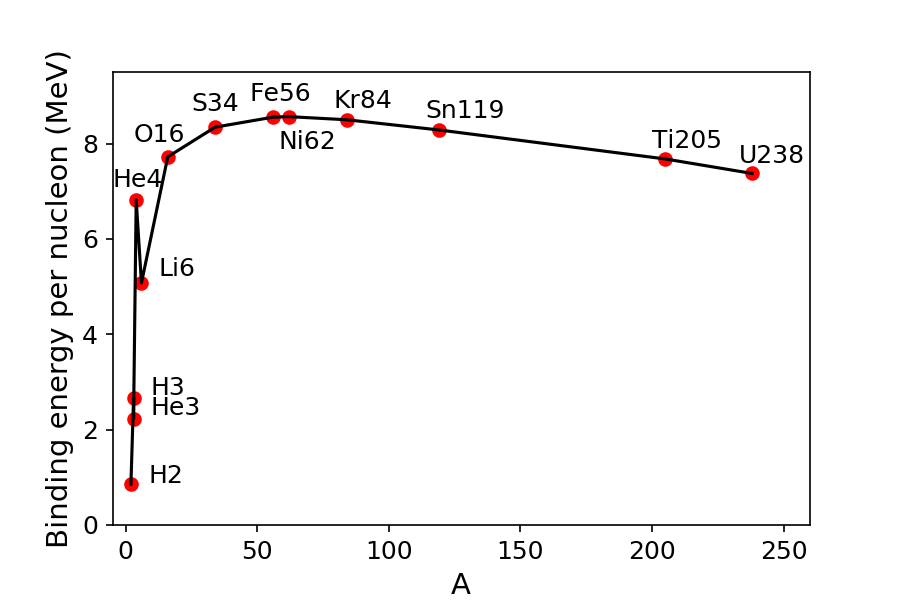
\includegraphics[scale=0.56] {figures/01-bindingcurve.png}}\protect
\caption{\label{fig:binding} \footnotesize{Binding energy per nucleon for selected nuclides. ${}^{62}\text{Ni}$ is the most bounded nuclide.}}
\end{figure}


The average binding energy can be approximated with the semi-empirical Bethe–Weizs\"acker formula, which is based on the liquid drop model of the nucleus and has various, similar forms in literature with slightly different values. Here we use one from [Anglart]

\begin{equation}
BE(A,Z)=15.75A-17.8A^{2/3}-94.8\frac{(A/2 - Z)^2}{A}-0.71Z^2A^{-1/3}+34\delta A^{-3/4}
\end{equation}

where $\delta = 1$ for even-even nuclei, $\delta = -1$ for odd-odd nuclei and $\delta = 0$ otherwise. The constants are in MeV. The relevance of this formula is that it gives some heuristic explanation of the binding energy.

\begin{itemize}
\item 1st, volume term: inside the "drop" all nucleons have more neighbors, therefore it is bonded to more nucleons. If all nucleons would be inside the drop they would feel the force of all other nucleons, therefore the binding energy would increase with $\propto A$
\item 2nd: surface term: nucleons on the surface will have less neighbors, therefore they experience lower binding energy. The number of such nucleons is proportional to the surface $\propto R^2=A^{2/3}$
\item 3rd: Symmetry term: due to the Pauli principle one energy level can be occupied only by two particles (with different spins), thus a different number of neutrons and protons result in excess energy. In fact if there was not the repulsive interaction of protons, ideally a nucleon would have the same number of protons and neutrons. The number of neutrons occupying higher levels than the protons is $N-Z$, and also the amount of excess energy of neutrons is proportional to $N-Z$. And the distance of the energy levels is $\propto 1/A$. For further explanation see [John Lilley: Nuclear Physics]. In total this energy is $\propto (N-Z)^2=(A-2Z)^2$. 
\item 4th, Coulomb term: protons will repel each other due to having the same electric charge $\propto \frac{Z^2}{R}=Z^2A^{-1/3}$
\item 5th, pairing term: Empirical observations show that nuclei having even number of protons or neutrons are more stable, especially if both are even. The reason is that similar nucleons like to be in pairs (this cannot be explained by the liquid drop model. 
\end{itemize}
 

\subsection{Nuclear reactions}

As said before there are two type of nuclear reactions important in the context of reactor physics:

\begin{itemize}
\item Spontaneous disintegration reactions (ie. decay reactions)
\item Collision reactions
\end{itemize}

\subsubsection{Decay reactions}

In decay processes the nucleus undergoes a transformation spontaneously  which results in the creation of an other nuclide. The process is accompanied by the emission of particles. The most common decay processes in nature are:

\begin{itemize}
\item $\alpha$-decay: a He nucleus is emitted for heavier nuclides (when the repulsive Coulomb force overcomes the attractive nuclear force)  ${}_Z^A\text{X} \rightarrow {}_{Z-2}^{A-4}\text{Y} + {}_2^4\text{He} + Q$.
\item $\beta^-$-decay: a neutron in the nucleus is transformed into a proton and an electron: ${}_Z^A\text{X} \rightarrow {}_{Z+1}^{A}\text{Y} + e^-+\bar\nu_e + Q$
\item $\beta^+$-decay: a proton in the nucleus is transformed into a neutron and a positron: ${}_Z^A\text{X} \rightarrow {}_{Z-1}^{A}\text{Y} + e^{+}+\nu_e + Q$
\item $\gamma$-decay: when the nucleus is in an excited state it can release energy in the form of $\gamma$ photons to reach a lower energy level or the ground state. The energy of the gamma photons is characteristic to the nuclide. ${}_Z^A\text{X}^*\rightarrow {}_Z^A\text{X} + \gamma$
\item neutron emission: as we will see later in the course some nuclides emit a neutron following a $\beta$-decay. This process has a great importance in reactor physics.
\end{itemize}

\noindent in the decay some energy in the form of kinetic energy ($Q$) is released. The released energy can be calculated from the binding energy of the original nuclide and the products.

\begin{tcolorbox}
Exercise

$${}_{88}^{226}\text{Ra}\rightarrow {}_{86}^{222}\text{Rn}+{}_{2}^{4}\text{He}$$

The binding energies (in the datalab we will calculate the $\epsilon$ average binding energies

$BE({}_{88}^{226}\text{Ra})=7.66196\cdot 226=1731.60296 \: MeV$

$BE({}_{86}^{222}\text{Rn})=7.69449\cdot 222=1708.17678 \: MeV$

$BE({}_{2}^{4}\text{He})=7.073922\cdot 4=28.295688 \: MeV$

Thus the total energy released

$$Q=[BE({}_{86}^{222}\text{Rn})+BE({}_{2}^{4}\text{He})]-BE({}_{88}^{226}\text{Ra})=4.8695 \: MeV$$

which is an enormous amount of energy. Let's consider that 1kg of ${}_{88}^{226}\text{Ra}$ decays. The number of nuclei is

$N=\frac{mN_A}{M}=2.6\cdot 10^{24}$

\noindent where $N_A$ stands for Avogadro's number, thus the total released energy would be

$E=NQ=2028 \: GJ$

Of course as we will see soon, this energy is released over thousands of years.
\end{tcolorbox}



\begin{figure}[ht!]
\protect \centering{
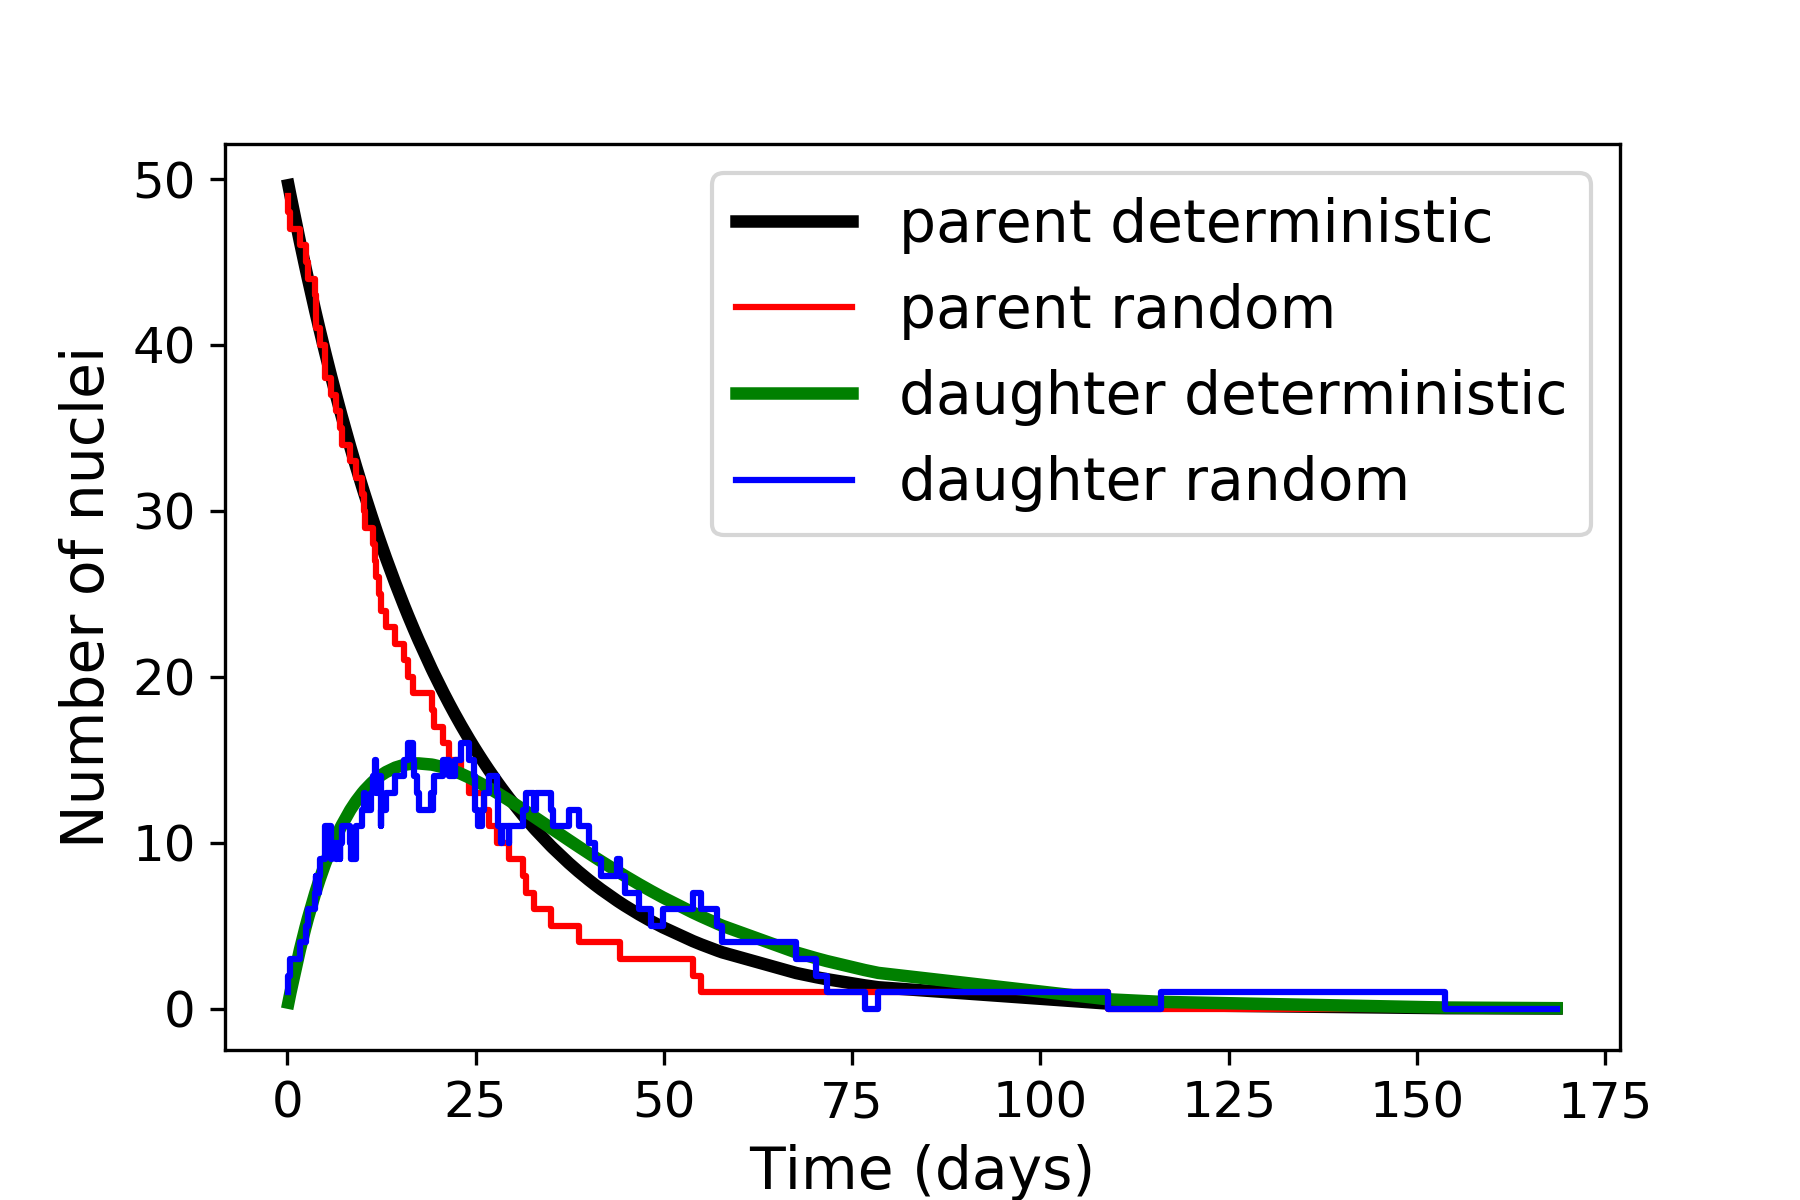
\includegraphics[scale=0.46] {figures/01-radioactivdecay_daughterparent.png}
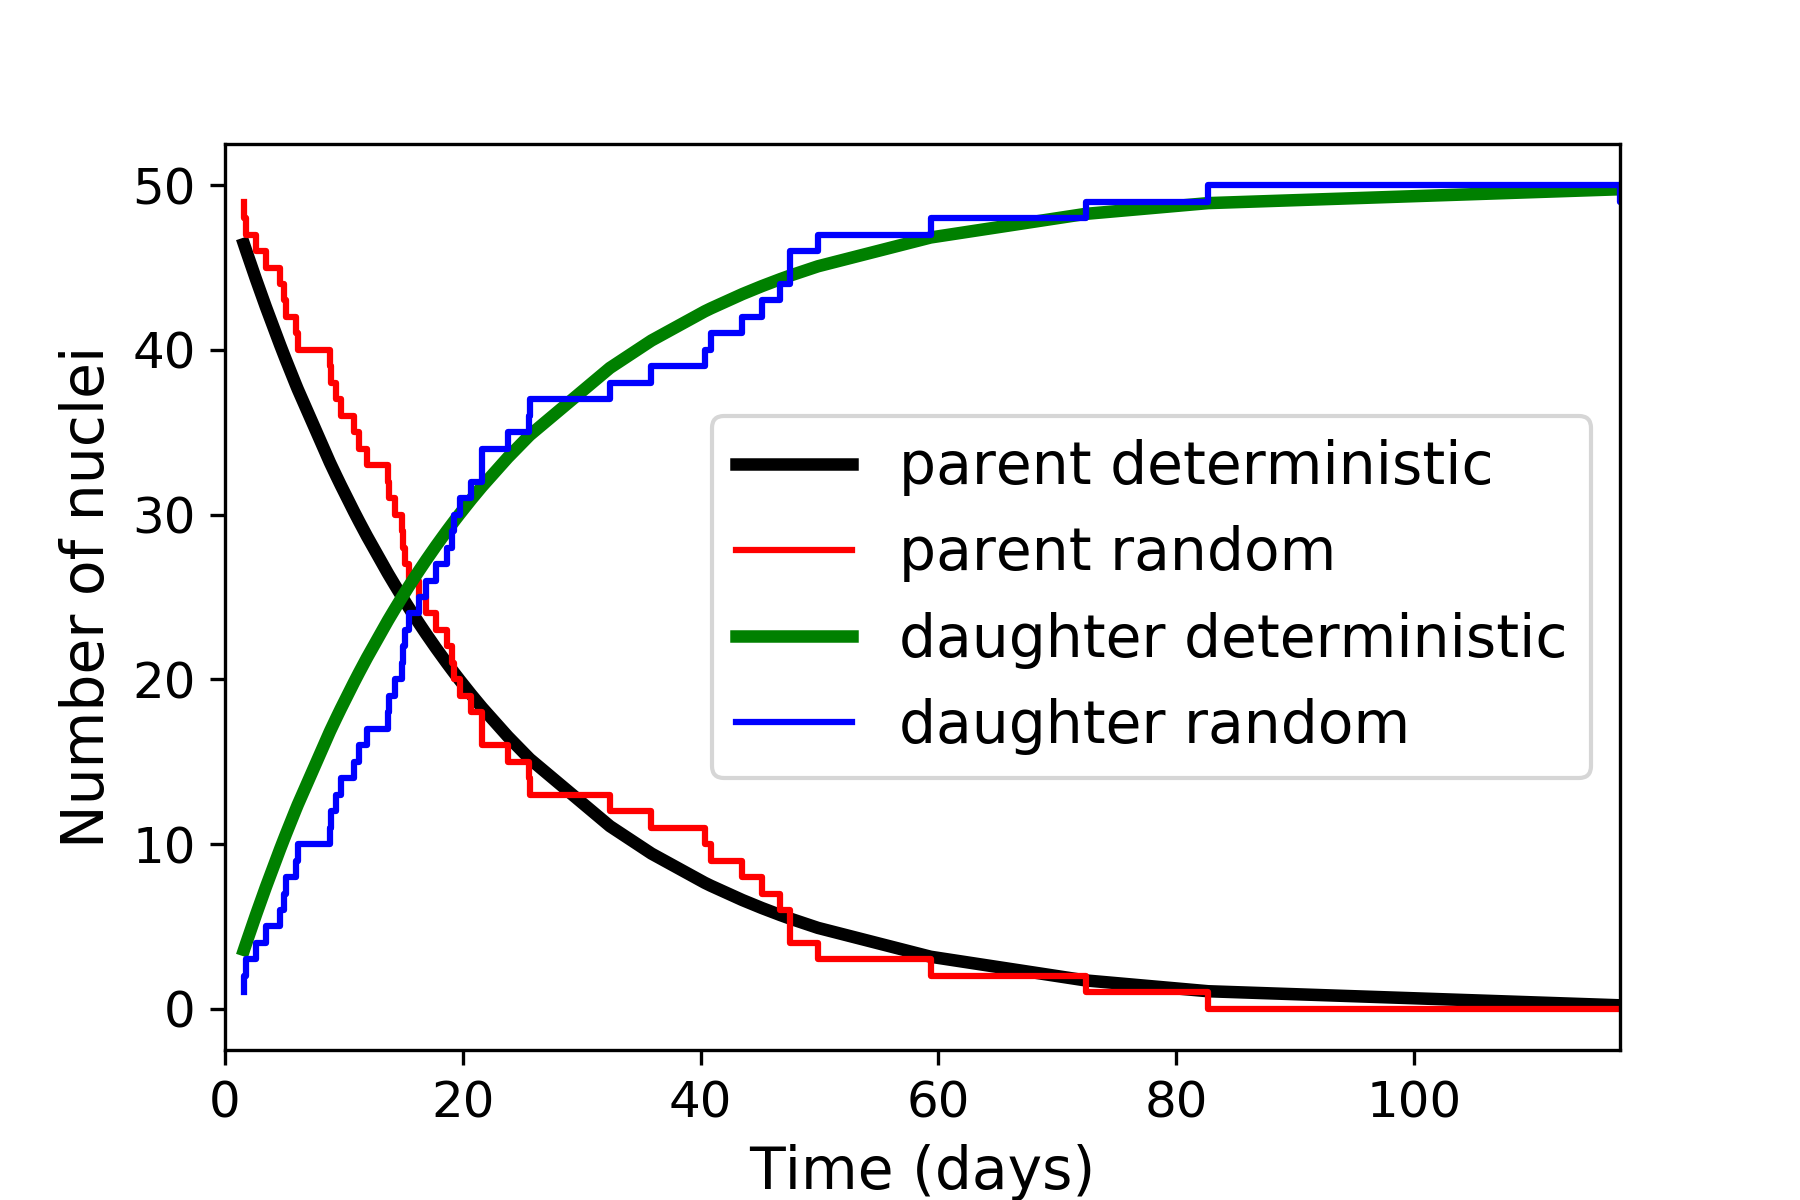
\includegraphics[scale=0.46] {figures/01-radioactivdecay_daughterparent_LongDaughter.png}}\protect
\caption{\label{fig:decay} \footnotesize{Decay of parent and daughter nuclide (Random notes a case when the decay times are sampled from an exponential distribution). Top: $T_{1/2,P} > T_{1/2,D}$. Bottom	: $T_{1/2,P} << T_{1/2,D}$}}
\end{figure}

The fundamental law of decay is that (based on observations) the probability of the decay of a nucleus in a given time interval is constant. This means that the chance to decay does not depend on the age of the nucleus. In other words, if we have more nuclei, the rate of decays (or the change in the number of nuclei in time) is proportional to the number of nuclei:

\begin{equation}
\frac{dN}{dt}=-\lambda N(t)
\end{equation}

\noindent where the decay constant $\lambda \: [s^{-1}]$ is characteristic to the type of nuclide and where $N(t)$ is the number of nuclei. However often it is more practical to write up such equation for the number density (in $\#/cm^3$). The solution to this equation is

\begin{equation}\label{eq:decay}
N(t)=N_0e^{-\lambda t}
\end{equation}

\noindent with some initial number of nuclei (or number density) $N_0=N(t=0)$. Therefore rate or as often called the activity is

\begin{equation}
\text{Rate}=A(t)=\lambda N(t)=\lambda N_0e^{-\lambda t}
\end{equation}

The activity has its units in $s^{-1}=Bq$, however in some older texts one can encounter the unit $Ci=3.7 \cdot 10^{10}\: Bq$. The $Ci$ is defined so that $1 \: Ci$ is the activity of 1g of Radium. We can clearly see that the activity of a sample depends both on the type of nuclides in the sample (due to the decay constant) and also on the quantity of radionuclides in the sample.

Although these equations are deterministic, however as said before radioactive decay is a stochastic process. An other way to interpret these equations is to consider that the probability of decay during the time interval $(t,t+dt)$ for a given nucleus is

\begin{equation}
p(t)dt=\lambda e^{-\lambda t}dt
\end{equation}

Therefore the time measured from some starting moment, when a single nucleus disintegrates follows an exponential distribution. Fig. \ref{fig:decay} shows the decay of nuclei over time both by solving the problem with a deterministic approach (ie. by illustrating Eq. \eqref{eq:decay}) and with a stochastic approach (ie. when decay times are sampled from an exponential distribution. 

Although the life-time of a radioactive nuclei is stochastic, but we can calculate the average life-time.

\begin{equation}
\bar{t}=\int\limits_0^\infty{t\cdot p(t) dt}=\frac{1}{\lambda}
\end{equation}

However in practice, usually a more convenient quantity, called half-life is defined as the time while the number of nuclei (or the number density) becomes half of its initial value:

\begin{equation}
N(T_{1/2})=\frac{N_0}{2}=N_0e^{-\lambda T_{1/2}}
\end{equation}

from where we can express the half-life with the decay constant

\begin{equation}
T_{1/2}=\frac{\ln(2)}{\lambda}
\end{equation}

However in practice we usually have more complicated situations, when some nuclide $A$ will decay into an other nuclide $B$ which then decays into a third type of nuclide $C$, and a chain of events happen until all the initial nuclide is not transformed into a stable nuclide through several decay reactions. Also we often have some production of initial nuclides (for example the production of ${}^{14}C$ in the atmosphere due to collision reactions). We will discuss such processes in more detail later when discussion the time evolution of nuclear fuel during operation. For the moment let us only consider a simple situation when a parent nuclide $P$ decays into a radioactive daughter~$D$. One can see that the logic of solving this problem can be easily generalized for several daughters. We just need to solve a set of coupled ordinary differential equations, which often we can do analytically, and easily solve it numerically (as will be shown during the datalabs). The only difficulty might be encountered that the decay constants can have very different order of magnitudes (which might cause numerical issues).

\begin{tcolorbox}
\textbf{Exercise}

Consider the decay process of a parent decaying into a daughter which then decays into a stable product: $P\rightarrow D \rightarrow S$, where the decays are characterized by $\lambda_P$ and $\lambda_D$.

We can write up the governing differential equations:

$$\frac{dN_P}{dt}=-\lambda_P N_P(t)$$

$$\frac{dN_D}{dt}=-\lambda_D N_D(t) + \lambda_P N_P(t)$$

\noindent with initial condition $N_P(t=0)=N_P(0)$ and $N_D(t=0)=0$. Hence the difference compared to \eqref{eq:decay} is that a production term appeared in the equation describing the rate of the daughter nuclide.

The solution of this coupled system of ODE

$$ N_{P} (t) = N_P(0)e^{-\lambda_{P}t}$$

$$ N_{D} (t) = \frac{\lambda_P}{\lambda_P - \lambda_{D}}N_P(0)(e^{-\lambda_{D}t} - e^{-\lambda_{P}t}) $$

The analytic solution of this problem is shown for different decay constants in Fig. \ref{fig:decay} for different decay constants. What is important to notice here is that in case the daughter has a much short half-life than the parent nuclide, then the activity of the two nuclides will be the same (as soon as a daughter is produced it decays away). This is called \textit{secular equilibrium}.
\end{tcolorbox}

\subsubsection*{Decay series}

As mentioned above, in practice usually we encounter longer decay chains, an example to that are the decay series of the naturally occurring radionuclides ${}^{235}\text{U}$, ${}^{238}\text{U}$, ${}^{232}\text{Th}$ and ${}^{237}\text{Np}$ (however due to the relatively short half-life of ${}^{237}\text{Np}$ - compared to the age of Earth -, only a couple of nuclides of the last series occur in nature). Fig. \ref{fig:decaychain} illustrates the Actinium series (ie. the decay chain of ${}^{235}U$). One can observe that several decay events lead to the final stable product ${}^{207}Pb$.


\begin{figure}[ht!]
\protect \centering{
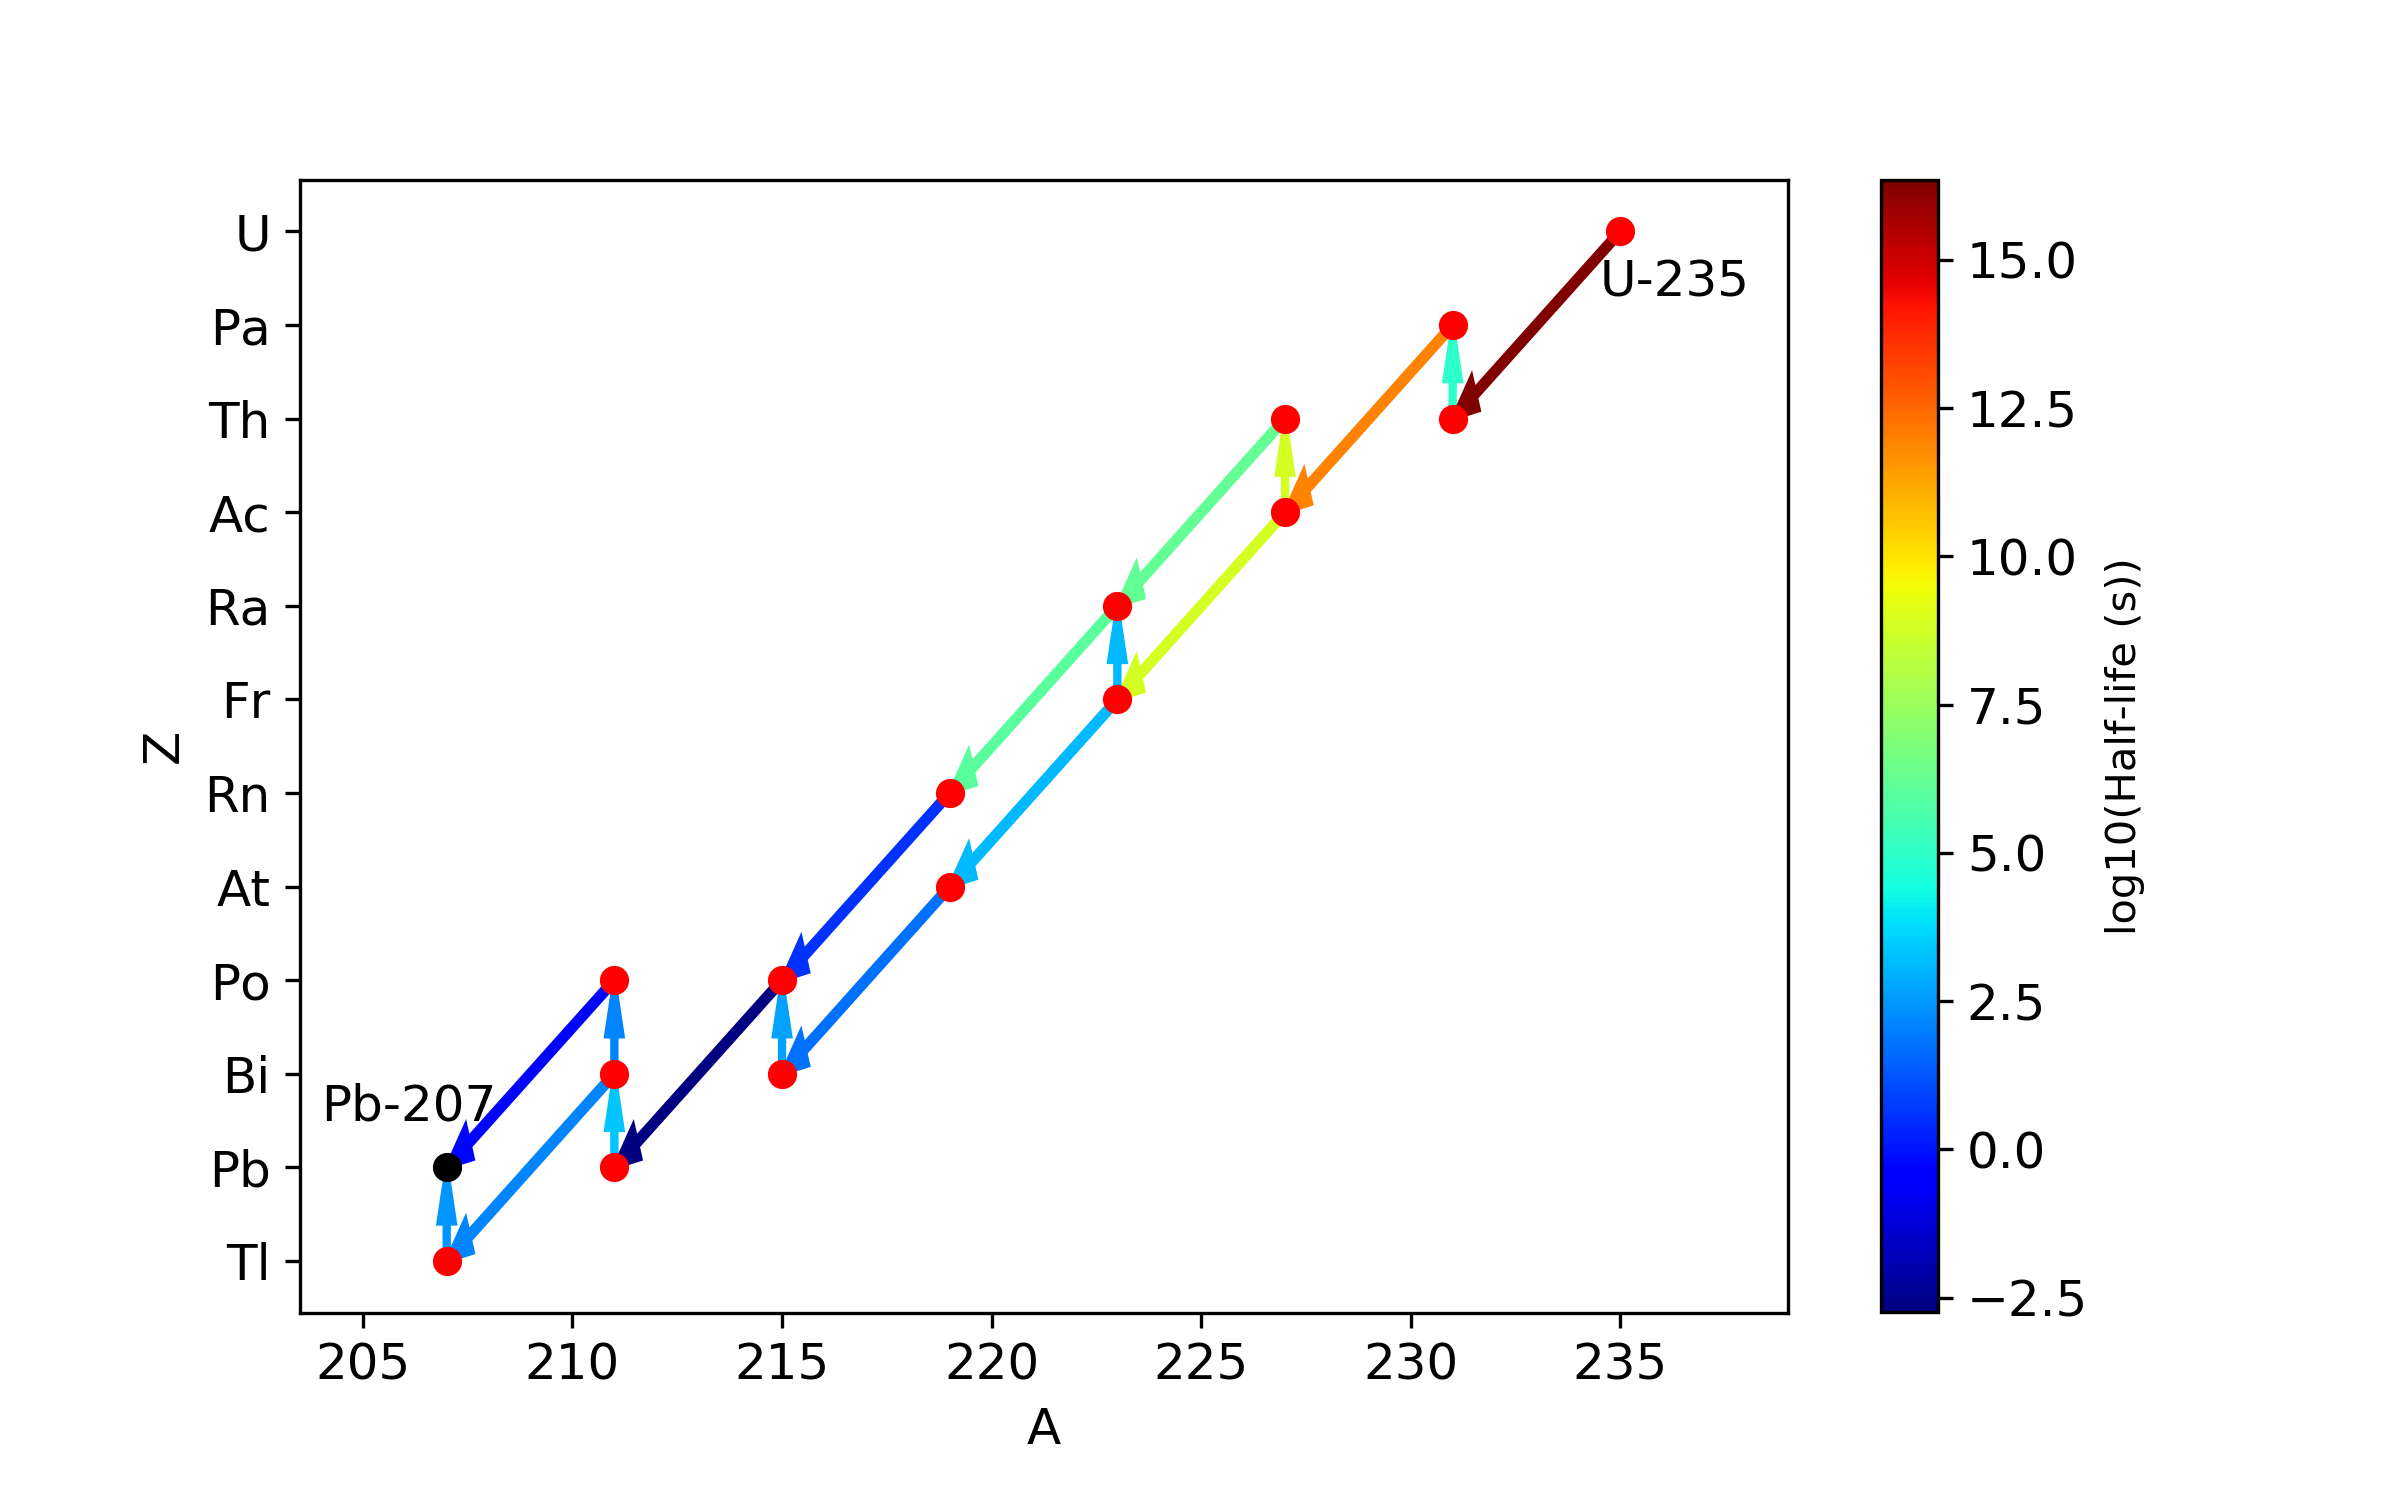
\includegraphics[scale=0.46] {figures/01-u235_decayseries.png}}\protect
\caption{\label{fig:decaychain} \footnotesize{${}^{235}U$ decay series.}}
\end{figure}

\subsubsection*{$\gamma$ decay}

As mentioned before $\gamma$ radiation is emitted during the transition between excited states. We can consider this reaction to be similar to a decay process, and characterize it with some decay constant $\lambda$. However, in this case due to quantum mechanical considerations we have to introduce the uncertainty or width $\Gamma$ of the energy level of the excited state. This width is related to the life time

\begin{equation}
\Delta E \Delta t \geq \hbar \rightarrow \Gamma=\hbar \lambda
\end{equation}

\subsection{Nuclear collision reactions}

When studying nuclear collision reactions between particles we can introduce similar notation as for chemical reactions:

\begin{equation}\label{eq:reaction}
a+X \rightarrow Y+b
\end{equation}

However in reactions relevant in reactor physics, one of the particles is often considered as a projectile and the other as a target (for example in the reactor the projectile, the neutron moves around in the system, whereas the target is often bound the a given location and changes locations only due to temperature induced fluctuations, for example U atoms in the fuel). In such reactions typically the outgoing particles can also be well distinguished in mass and type, however there are reactions (for example fission), where more particles appear after the reaction. A simple illustration of a nuclear collision reaction is given in Fig. \ref{fig:reactions}

\begin{figure}[ht!]
\protect \centering{
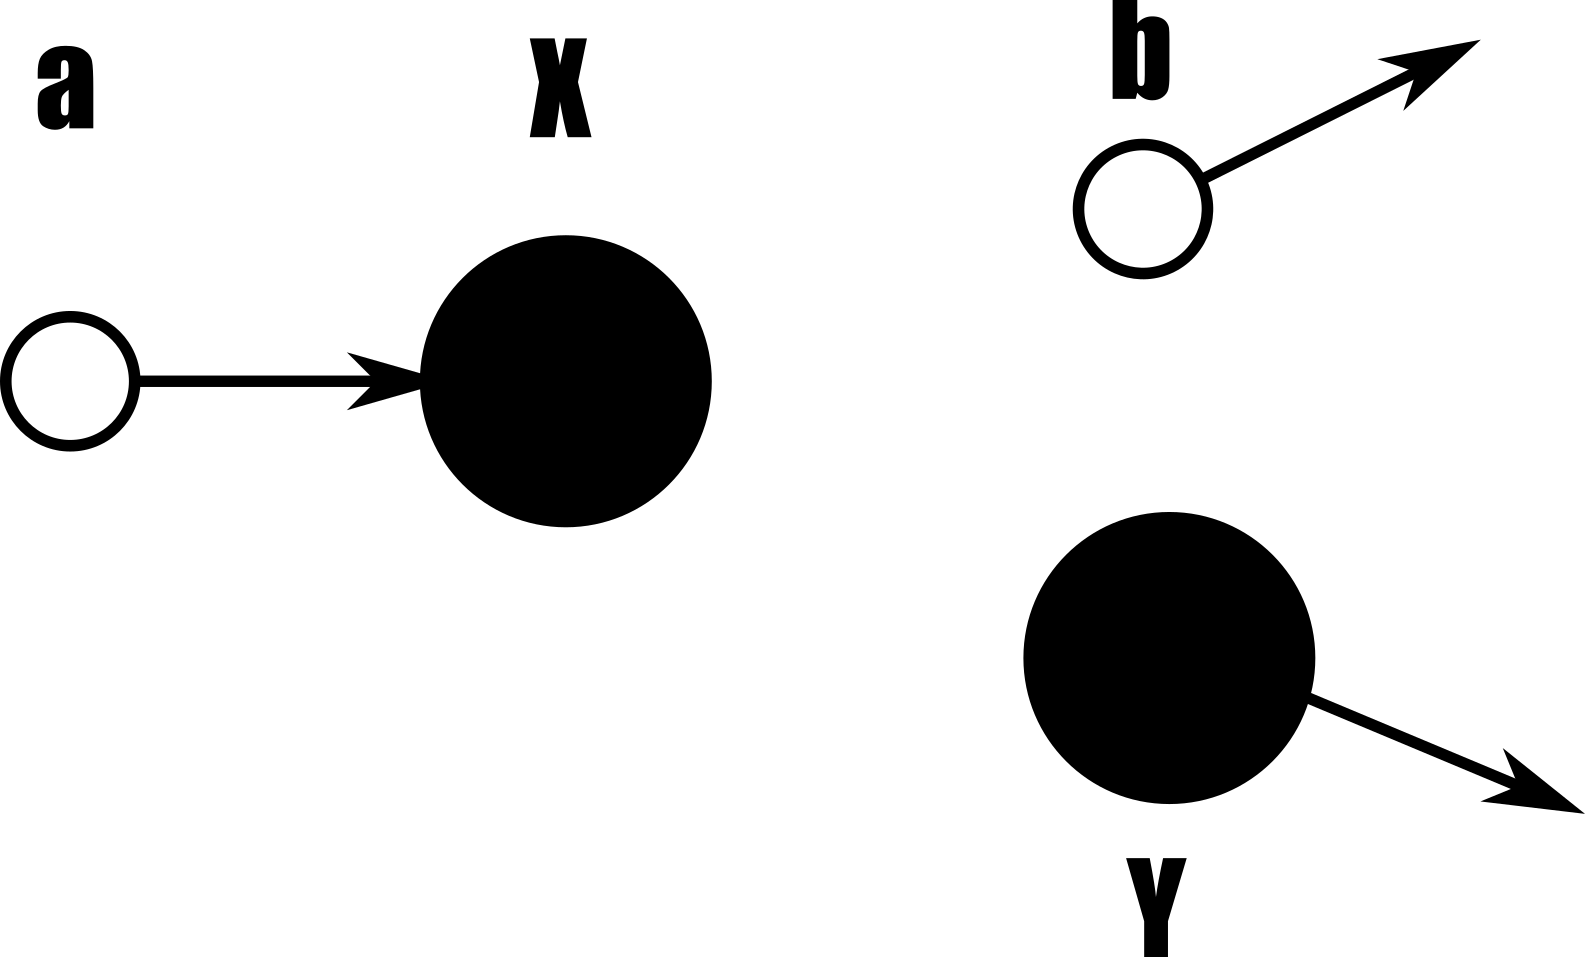
\includegraphics[scale=0.46] {figures/01-reactions.png}}\protect
\caption{\label{fig:reactions} \footnotesize{Illustration of nuclear collision events.}}
\end{figure}

Such reactions are often shorthanded as

\[
X(a,b)Y
\]

for example the neutron capture reaction on ${}_{92}^{235}U$ can be written as:

\[
{}_{92}^{235}U(n,\gamma){}_{92}^{236}U
\]

In general this class of reactions are often referred to as $(n,\gamma)$.

Since nuclear collision reactions are usually accompanied by the release or absorption of energy, it is often included in the notation. For the reaction \eqref{eq:reaction} one can calculate the reaction energy as

\begin{equation}\label{eq:reactionQ}
Q=[(m_a+M_X)-(M_Y+m_b)]c^2
\end{equation}

where Q is often referred to as the \textit{Q-value}. If $Q>0$, energy is released and the reaction is \textit{exothermic}. If $Q<0$, energy is required for the reaction to occur, the reaction is \textit{endothermic}.

As said before, there is a large variety of possible nuclear reactions, however the ones which are relevant for reactor physics involve the interaction of a neutron (as a projectile) and nuclei. These are

\begin{itemize}
\item Nuclear fission, $(n,fission)$
\item Radiative capture, $(n,\gamma)$
\item Elastic scattering, $(n,n)$ (the state of the target nucleus does not change)
\item Inelastic scattering, $(n,n')$ (the target nucleus becomes excited or a $\gamma$ photon is emitted promptly)
\item Several other reactions such as $(n,\textit{i}n)$, where $i$ number of neutrons are emitted from the target. $(n,p)$ and $(n,\alpha)$, where a proton or an $\alpha$ particle is emitted
\end{itemize}

As we will see later in light water reactors the fission, capture and elastic scattering reactions are dominating.

\subsection{Center of Mass vs LAB frame}

When we think about collision reactions, most naturally we imagine these in the laboratory or LAB frame, which means that the observer (for example we) is at a fixed point and always at rest. This is a rather intuitive frame, something we are used to since high school. However, the mathematical description of collision reactions it is often simpler in the center-of-mass or CM (sometimes CoM) frame, when the observer is at the center of mass of the system. 

\begin{figure}[ht!]
\protect \centering{
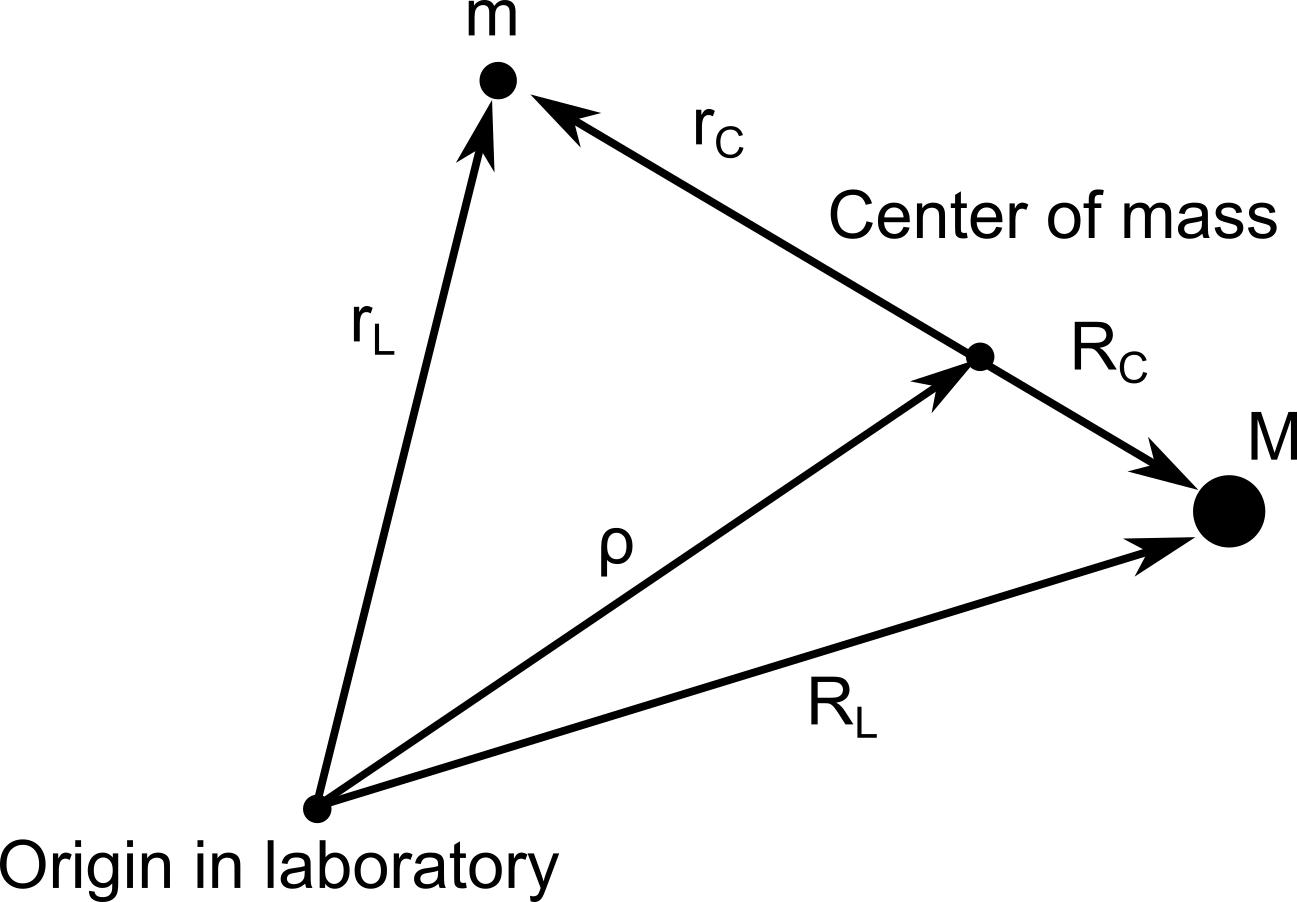
\includegraphics[scale=0.46] {figures/01-CoM.png}}\protect
\caption{\label{fig:LABCM} \footnotesize{LAB and CM frames.}}
\end{figure}

Let's consider the nucleus with mass $M$ at location $\mathbf{R}_L$ in the LAB frame and a neutron with mass $m$ at the location $\mathbf{r}_L$ in the LAB frame as illustrated in Fig. \ref{fig:LABCM}. We can then get the location of the center-of mass as 

\begin{equation}
\mathbf{\rho} = \frac{m\mathbf{r}_L+M\mathbf{R}_L}{m+M}
\end{equation}

from which we can convert the locations from LAB to CM as 

\begin{equation}
\mathbf{r}_C=\mathbf{r}_L - \mathbf{\rho}
\end{equation}

\noindent and

\begin{equation}
\mathbf{R}_C=\mathbf{R}_L - \mathbf{\rho}
\end{equation}

\noindent also

$$m\mathbf{r}_c + M\mathbf{R}_c = \mathbf{0}$$

We get similar formula for the velocities of the center of mass if we consider that the velocities in the LAB are $\mathbf{v}_L$ and $\mathbf{V}_L$ for the neutron and the nucleus. The center-of-mass travels with a velocity of

\begin{equation}
\mathbf{v}_{CM} = \frac{m\mathbf{v}_L+M\mathbf{V}_L}{m+M}
\end{equation}

And with that $\mathbf{v}_C=\mathbf{v}_L - \mathbf{v}_{CM}$ and $\mathbf{V}_C=\mathbf{V}_L - \mathbf{v}_{CM}$. Using such a reference frame is not always intuitive, however if we imagine that the target nucleus is at rest (which is usually not the case, since the target moves due to temperature, however this velocity is negligible for fast enough neutron energies), so $\mathbf{V}_L=0$, then the formalism further simplifies:

\begin{equation}
\mathbf{v}_{CM}=\frac{m}{m+M}\mathbf{v}_L
\end{equation}

\begin{equation}
\mathbf{v}_C=\mathbf{v}_L-\mathbf{v}_{CM}=\frac{M}{m+M}\mathbf{v}_L
\end{equation}

and

\begin{equation}
\mathbf{V}_C=-\mathbf{v}_{CM}=-\frac{m}{m+M}\mathbf{v}_L
\end{equation}

Thus the total momentum in CM is $\mathbf{p}_C=m\mathbf{v}_C+M\mathbf{V}_C=\mathbf{0}$, which means that the vector $\mathbf{v}_C$ and $\mathbf{V}_C$ are co-linear. In case of a scattering event, in the CM the particles are traveling towards each other before, and they travel back to back from each other after the scattering. Since in the following sometimes we will refer to the CM frame, it was important to introduce it at this stage. However, later we will use and review this formalism further to study the kinematics of elastic scattering reactions.

\subsection{Neutron cross sections}

The probability that a neutron interacts with a nucleus is characterized by the quantity called nuclear cross sections. The knowledge of this probability is essential to assess how a population of neutrons is going to be traveling in a nuclear reactor. 

\subsubsection{Microscopic cross sections}

Imagine a thin foil (one atomic layer thick, so no nuclei is shielded by any other) being bombarded by a beam of neutrons which have the same speed and which travel to the same direction. The rate of neutron-nuclear reactions will be proportional to the intensity $I$ of neutrons and to the number of atoms per unit area $N_A$, and the proportionality is given by $\sigma$

%\begin{figure}[ht!]
%\protect \centering{
%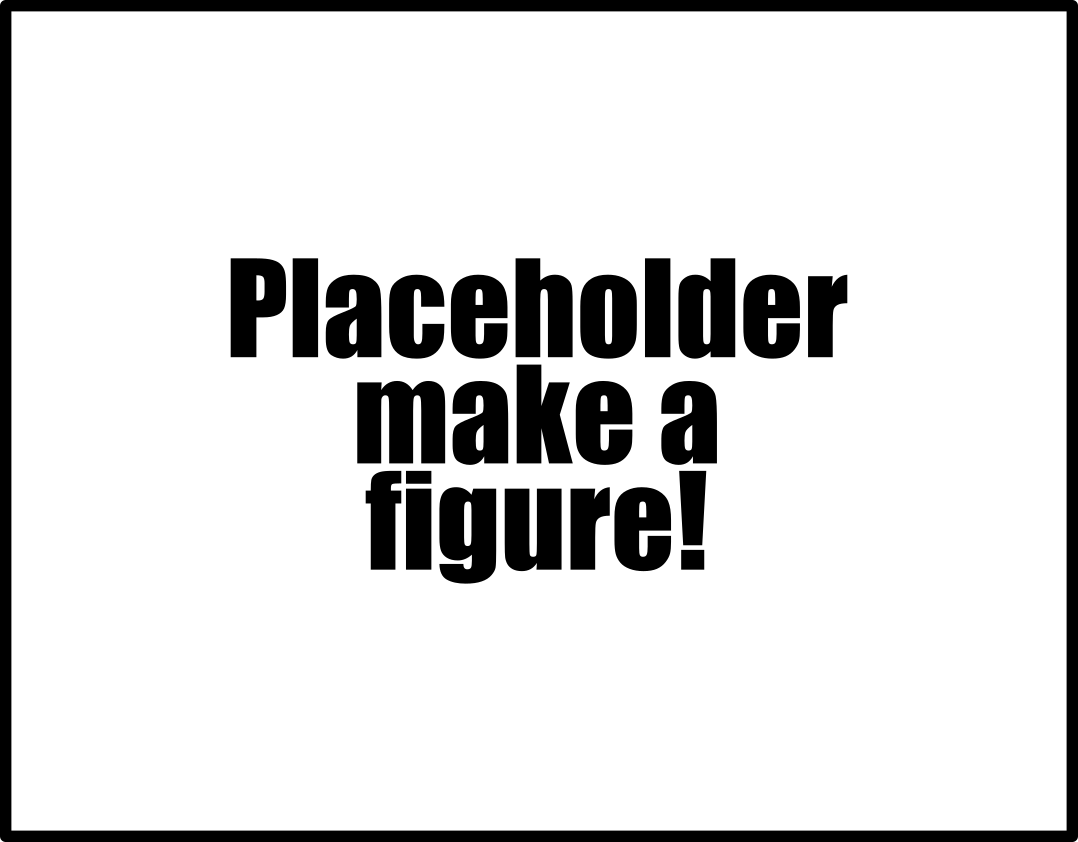
\includegraphics[scale=0.46] {figures/placeholder.png}}\protect
%\caption{\label{fig:beam} \footnotesize{Illustration of collimated mono-energetic neutrons bombarding a thin foil.}}
%\end{figure}

\begin{equation}
R[\frac{\#}{cm^2s}]=\sigma [cm^2] I [\frac{\#}{cm^2s}] N_A [\frac{\#}{cm^2}]
\end{equation}

thus\footnote{Some might be bothered that $\#\#$ should be $\#^2$, but mathematically speaking we could substitute $\#=1$, and physically speaking we have to see that in $I$ the number $\#$ refers to neutrons, in $N_A$ it refers to nuclei, and in $R$ it refers to the reaction, which indeed needs both a neutron and a nucleus.}

\begin{equation}\label{eq:sigma}
\sigma=\frac{R}{IN_A}=\frac{R/N_A}{I}=\frac{\text{Number of reactions per nucleus per second}}{\text{Number of incident neutrons per cm}^2\text{ per second}}
\end{equation}

If we imagine the neutrons and the nuclei as classical particles (like solid spheres), then the proportionality constant $\sigma$ would be the cross sectional area of a single nucleus, therefore we call it \textit{microscopic cross section}. If we consider that the radius of a nucleus has a magnitude of $10^{-12}$ cm, then the cross sectional area would have a magnitude of $10^{-24}$ cm$^2$. Microscopic cross sections are measured in units of $10^{-24}$ cm$^2$, which we call $barn$ (often shorthanded as $b$).

Nevertheless, neutrons and nuclei do not behave as classical particles, thus one needs to take into account the quantum mechanical nature of such reactions, so the geometrical interpretation of the cross section is not always correct. Due to resonance effects, some nuclei will have very different microscopic cross sections very different from the geometrical cross sections. 

%It is also clear, that the probability per nuclear that a neutron interacts with it is $\sigma/A$, where A is the total cross sectional area.

\begin{figure}[ht!]
\protect \centering{
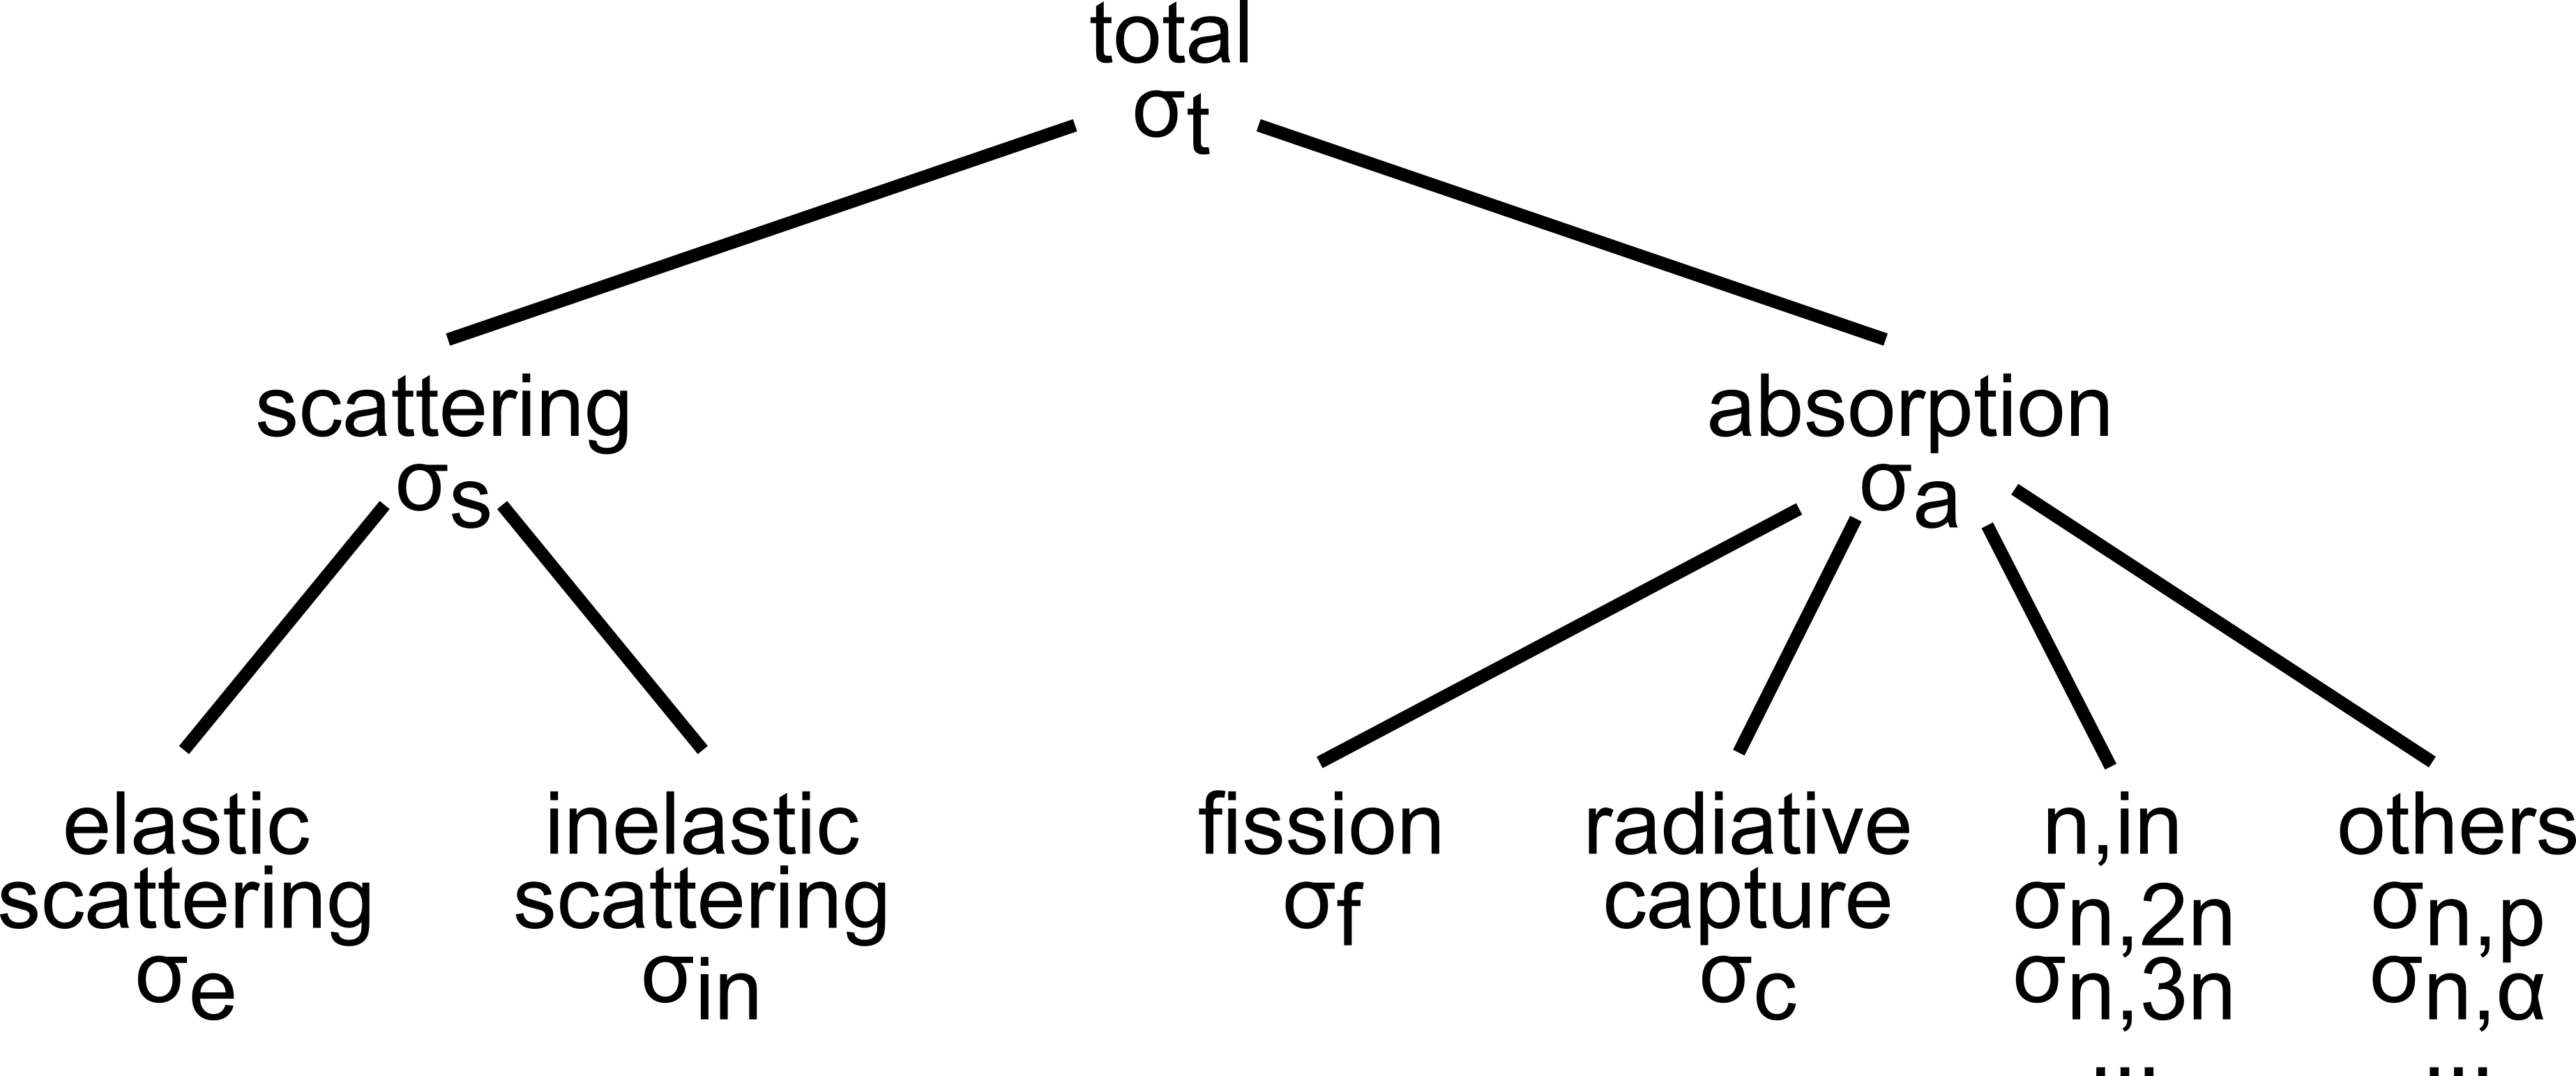
\includegraphics[scale=0.4] {figures/01-xshierarchy.png}}\protect
\caption{\label{fig:xshierarchy} \footnotesize{Hierarchy of reactions and cross sections.}}
\end{figure}

In a similar manner we could define microscopic cross sections for the various reaction types separately (eg. $\sigma_f$, $\sigma_e$ and $\sigma_c$ for fission, elastic scattering and capture respectively). Since this values are related to probabilities, we can sum them up, and define further cross sections, like the sum of elastic and inelastic scattering is the \textit{scattering cross section}

\[
\sigma_s=\sigma_e + \sigma_{in}
\]

or the sum of all cross sections is the \textit{total cross section}

\[
\sigma_t=\sigma_s + \sigma_{f}+ \sigma_{c} + ...
\]

which gives the probability that any reaction occurs. The absorption cross section can be define as 


\[
\sigma_a=\sigma_t - \sigma_s
\]

which gives the probability that a reaction resulting in the disappearance of the projectile neutron occurs. Note that some reactions will produce further neutrons, but as we will see when describing neutron transport usually we account for this by adding them separately. Fig. \ref{fig:xshierarchy} reviews the hierarchy of the cross sections. Note, that some textbooks consider (n,\textit{i}n) reactions as scattering reactions.

\subsubsection{Macroscopic cross sections}

In practical applications, such as in a nuclear reactor, the target is thicker than a foil (consider that a fuel pin is around a 1cm in diameter and is surrounded by few mm thick cladding and few cm of coolant and/or moderator material). In such situation most of the nuclei will be shielded by other nuclei, and the beam intensity changes inside the target. Let's look at an infinitesimally think layer between $[x,x+dx]$. The number of reactions in this layer is

\[
dR=\sigma_t I N dx
\]

\noindent where $N$ is the number density of nuclei. The change in the beam is therefore

\[
\frac{dI}{dx}=\frac{I(x+dx)-I(x)}{dx}=-\sigma_tI(x)N
\]

\noindent which, in case of $I(x=0)=I_0$ has the solution of

\[
I(x)=I_0\exp(-\sigma_tNx)
\]

Since the quantity $\sigma_t N$ appears often we prefer to introduce a new quantity, the \textit{macroscopic cross section}:

\[
\Sigma_t=\sigma_tN=[cm^{2}cm^{-3}=cm^{-1}]
\] 

\noindent which is related to the probability of interaction in a macroscopic sample (remember: the microscopic cross section was related to the probability of interaction per nucleus). However, this quantity is a cross section only in name. As we see it has inverse length units, and indeed it is rather related to the probability that an interaction happens over a certain distance traveled by the neutron. In fact

\begin{itemize}
\item $\exp(-\Sigma_t x)$ is the probability that a neutron travels a distance dx without participating in any interaction.
\item $\Sigma_t \exp(-\Sigma_t x)dx=p(x)dx$ is the probability that the neutron has suffers an interaction at dx.
\end{itemize}

One can notice that $p(x)$ is a probability density function. Later we will learn how to sample such probability density function to sample random path lengths between collisions. For the moment we can however notice that it is possible to calculate the mean free path $\bar\lambda$ from

\[
\bar\lambda=\int\limits_0^\infty xp(x)dx=\frac{1}{\Sigma_t}
\]

Similarly we could define the collision frequency for neutrons traveling with speed $v$ as $v\Sigma_t$ and the mean time between interactions as $\frac{1}{v\Sigma_t}$.

The definition of macroscopic cross sections can be generalized to other reactions, for example fission ($\Sigma_f=N\sigma_f$), absorption ($\Sigma_a=N\sigma_a$) or scattering $\Sigma_s=N\sigma_s$, with which the total macroscopic cross section is

\[
\Sigma_t=\Sigma_a+\Sigma_s
\]

However the mean free path can be defined only for the total cross section (note that $\frac{1}{\Sigma_t} = \frac{1}{\sum\limits_i \Sigma_i}\neq \sum\limits_i\frac{1}{\Sigma_i}$)

One can also calculate the macroscopic cross section of homogeneous mixtures:

\[
\Sigma_t^{mix}=\sum\limits_i^M N_i\sigma_t^i \quad \text{for i=1,2,...M nuclides}
\]

\begin{tcolorbox}
\textbf{Exercise}

Consider a control rod made of boron carbide ($\text{B}_4\text{C}$) with natural boron. Natural boron consists of two stable isotopes: B-11 (80.1\%) and B-10 (19.9\%). Determine the total macroscopic cross-section and the mean free path of a neutron in boron carbide if
\begin{itemize}
\item $\rho = 2.52\text{g}/\text{cm}^3$
\item $M_B = 10.8\text{g}/\text{mol}$
\item $M_C = 12\text{g}/\text{mol}$
\item $\sigma_{\text{B-10}}=3843 \text{b}$, $\sigma_{\text{B-11}}=5.07 \text{b}$, $\sigma_{\text{C-12}}=5.01 \text{b}$

$$\Sigma=\frac{\rho N_A}{M_{B_4C}}\sum_in_i\sigma_i$$
$$\Sigma=\frac{\rho N_A}{4M_{B}+M_{C}}(4\sigma_B+\sigma_C)$$
$$\Sigma=\frac{\rho N_A}{4M_{B}+M_{C}}(4(0.801\sigma_{B-11}+0.199\sigma_{B-10})+\sigma_C)=84.4 \: \text{cm}$$
$$\lambda=\frac{1}{\Sigma}=0.11\:\text{mm}$$
\end{itemize}
 \end{tcolorbox}

As we will see shortly, the microscopic cross section has strong dependence on the neutron energy, therefore the macroscopic cross section also has the same dependence. However, the number density can have strong variations in space and in time as well (for example reactors are heterogeneous systems, so the material composition varies between various locations, and as we will see later, over time due to depletion the composition does change), therefore the macroscopic cross sections often also have strong dependence on these variables:

\[
\Sigma (E, r, t)=N(r,t)\sigma (E)
\]

\subsubsection{Reaction rate and flux}

As stated above, the collision frequency for neutrons traveling with speed $v$ is 

\begin{equation}
\text{collision frequency}=v\Sigma_t
\end{equation}

\noindent Now, let's define the neutron population as 

\begin{equation}
n(t)=\text{Number of neutrons per unit volume }(1/\text{cm}^3)
\end{equation}

\noindent then the number of reactions over time and over volume unit volume would be

\begin{equation}
R(t)=\text{Reaction rate density}=n(t)v\Sigma_t \quad (1/(\text{cm}^3s))
\end{equation}

\noindent where the quantity $vn(t)$ appears so often in reactor physics that it is used to describe the neutron population and is called neutron flux

\begin{equation}
\phi(t)=\text{Neutron flux}=n(t)v\Sigma_t \quad (1/(\text{cm}^2s))
\end{equation}

As we will see later, the neutron flux and the neutron density can be introduced in a more general manner when they depend on the location, neutron energy, and even the direction the neutrons travel towards. Although the main reason for using the neutron flux to describe the neutron population is because it is a convenient variable, it does have a physical meaning: the total distance traveled in a volume per second by neutrons. Note that often the reaction rate $R$ is related to the reaction rate in $1/s$ units, some textbooks therefore highlight density like quantities as $R'''$, we will not follow this notation, and use $R$ regardless it is reaction rate or reaction rate density, nevertheless we will try to be transparent in the text.


\subsubsection{Characteristics of microscopic cross sections}

Previously we have assumed that the beam contains mono-energetic neutrons traveling to the same direction. This however is not the case in a nuclear reactor. Furthermore, the microscopic cross sections do depend strongly on the energy, and rather weakly on the direction of the neutrons. It is therefore important to review the characteristics of cross sections. Here we focus on the fundamental physical mechanism involved in collision events, and later we will also review the kinematics of collision.

There are two main mechanism interesting for reactor physics:

\begin{itemize}
\item Potential scattering: when a neutron does not penetrate the nucleus, only scatters of its force field.
\item Compound nucleus formation: when the neutron penetrates the nucleus, and a new nucleus with $A+1$ is created, which then disintegrates either by emitting gamma photons, neutrons or undergoes fission.
\end{itemize}

Potential scattering can be handled in classical terms, as we will see later. The magnitude of the cross section for this reaction is essentially the geometrical cross section of the nucleus, and the energy dependence is flat over a wide range of energies as shown in Fig. \ref{fig:h1scatter}. Later we will investigate the kinematics of these events further to understand how neutrons loose their energy in scattering events.

\begin{figure}[ht!]
\protect \centering{
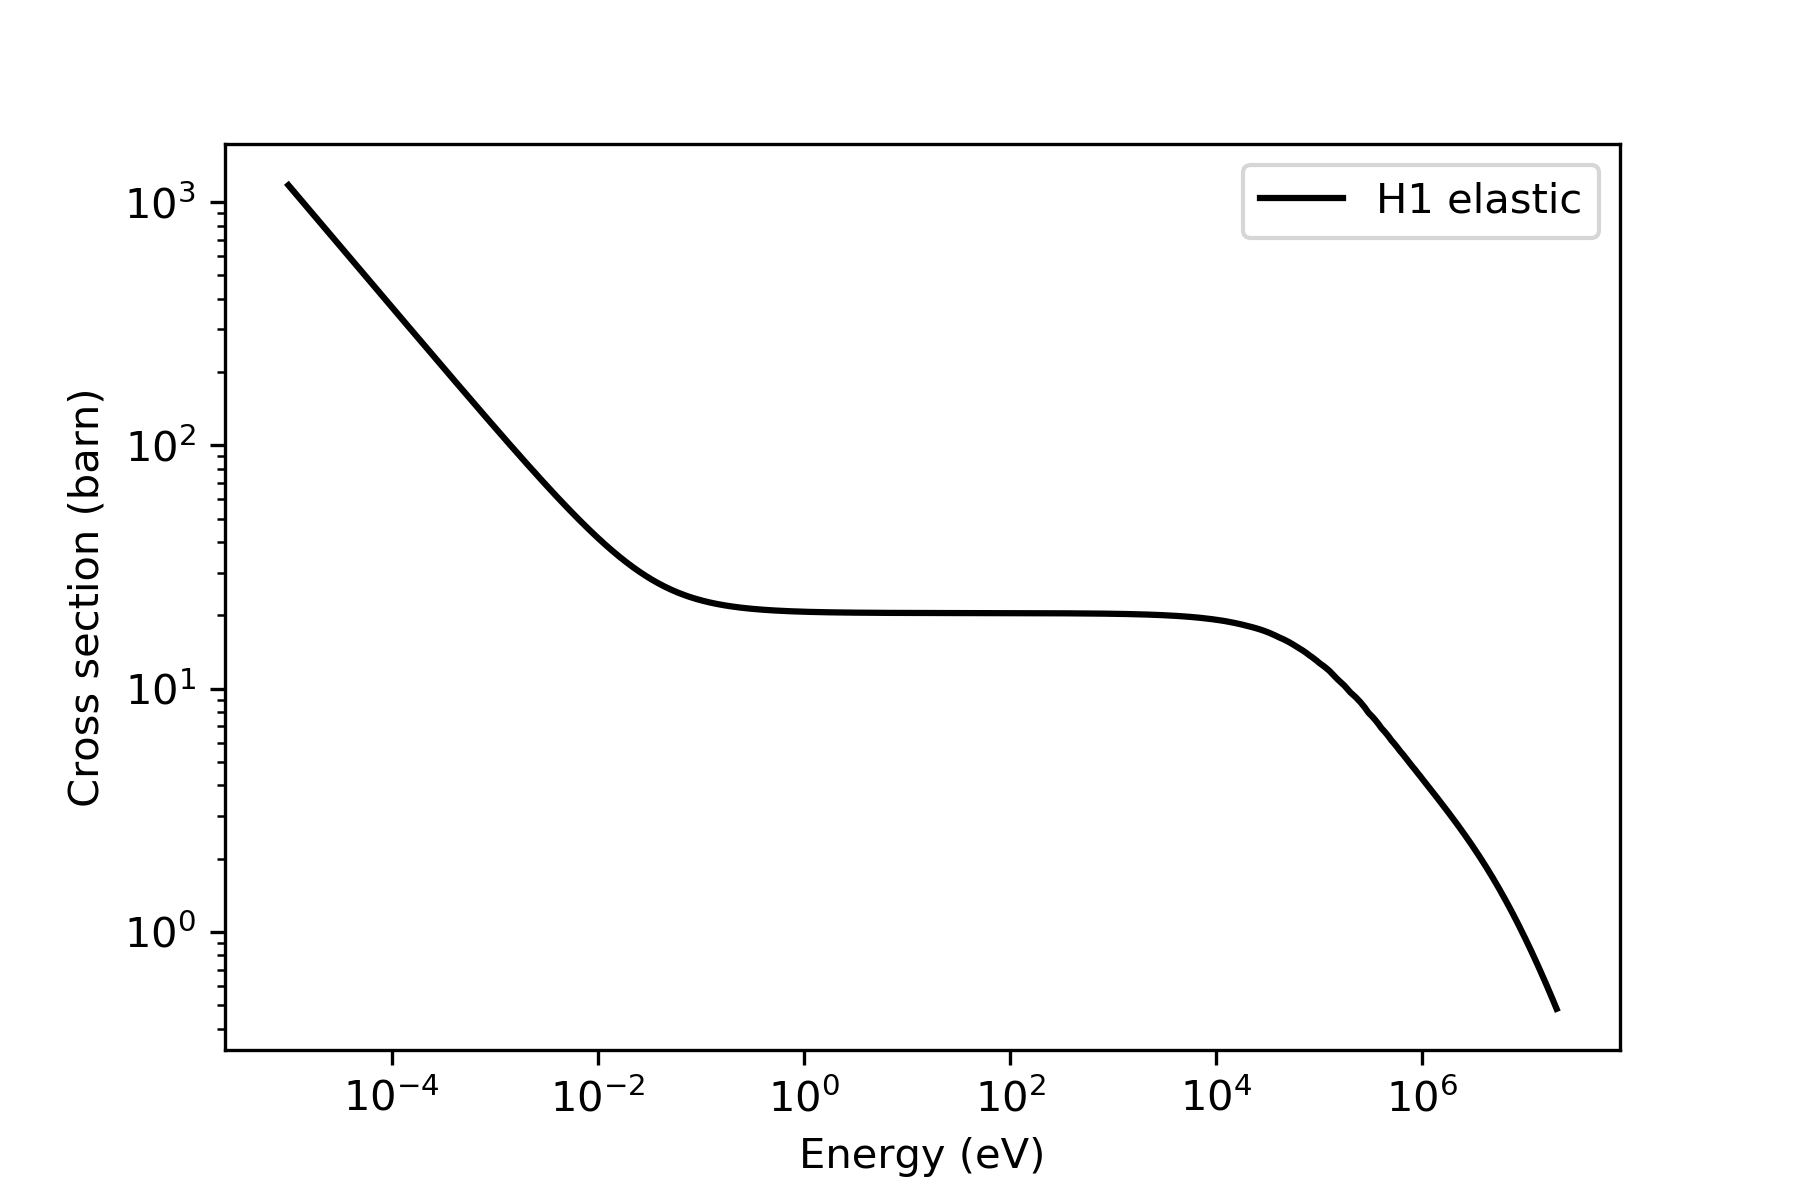
\includegraphics[scale=0.46] {figures/01-H1scattering.png}}\protect
\caption{\label{fig:h1scatter} \footnotesize{Elastic scattering cross section on Hydrogen-1.}}
\end{figure}

In compound nucleus formation however a new nucleus is formed. The time scale of this event is cca. 1000 times longer than it would take for the neutron to go through the nucleus. This tells us both that indeed something is happening there, and also this time is enough for the outcoming particles to "forget" what happened with them before (for example the the direction of the incoming neutron). Compound nucleus formation happens in many reactions: in fission, radiative capture and scattering:

\begin{equation}
    {}_Z^AX + n \rightarrow {}_Z^{A+1}X^*
    \begin{cases}
      a: \text{elastic scattering} \\
      b: \text{inelastic scattering} \\
      c: \text{radiative capture} \\
      d: \text{fission}
    \end{cases}
\end{equation}
    
In compound nucleus formation if the CM energy of the neutron plus the binding energy ($[M(A+1,Z)-M(A,Z)-m_n]c^2$) of the neutron matches an energy level of the compound nucleus than the magnitude of the cross section increases (often with several orders of magnitude). This is shown in Fig. \ref{fig:nalevels} for the capture cross section of Na-23. Then we refer to the "resonance" of Na-23, eventhough fundamentally the resonance corresponds to the energy level of the compound Na-24 nucleus. Resonances have different width, which depends on the lifetime of the energy level.

\begin{figure}[ht!]
\protect \centering{
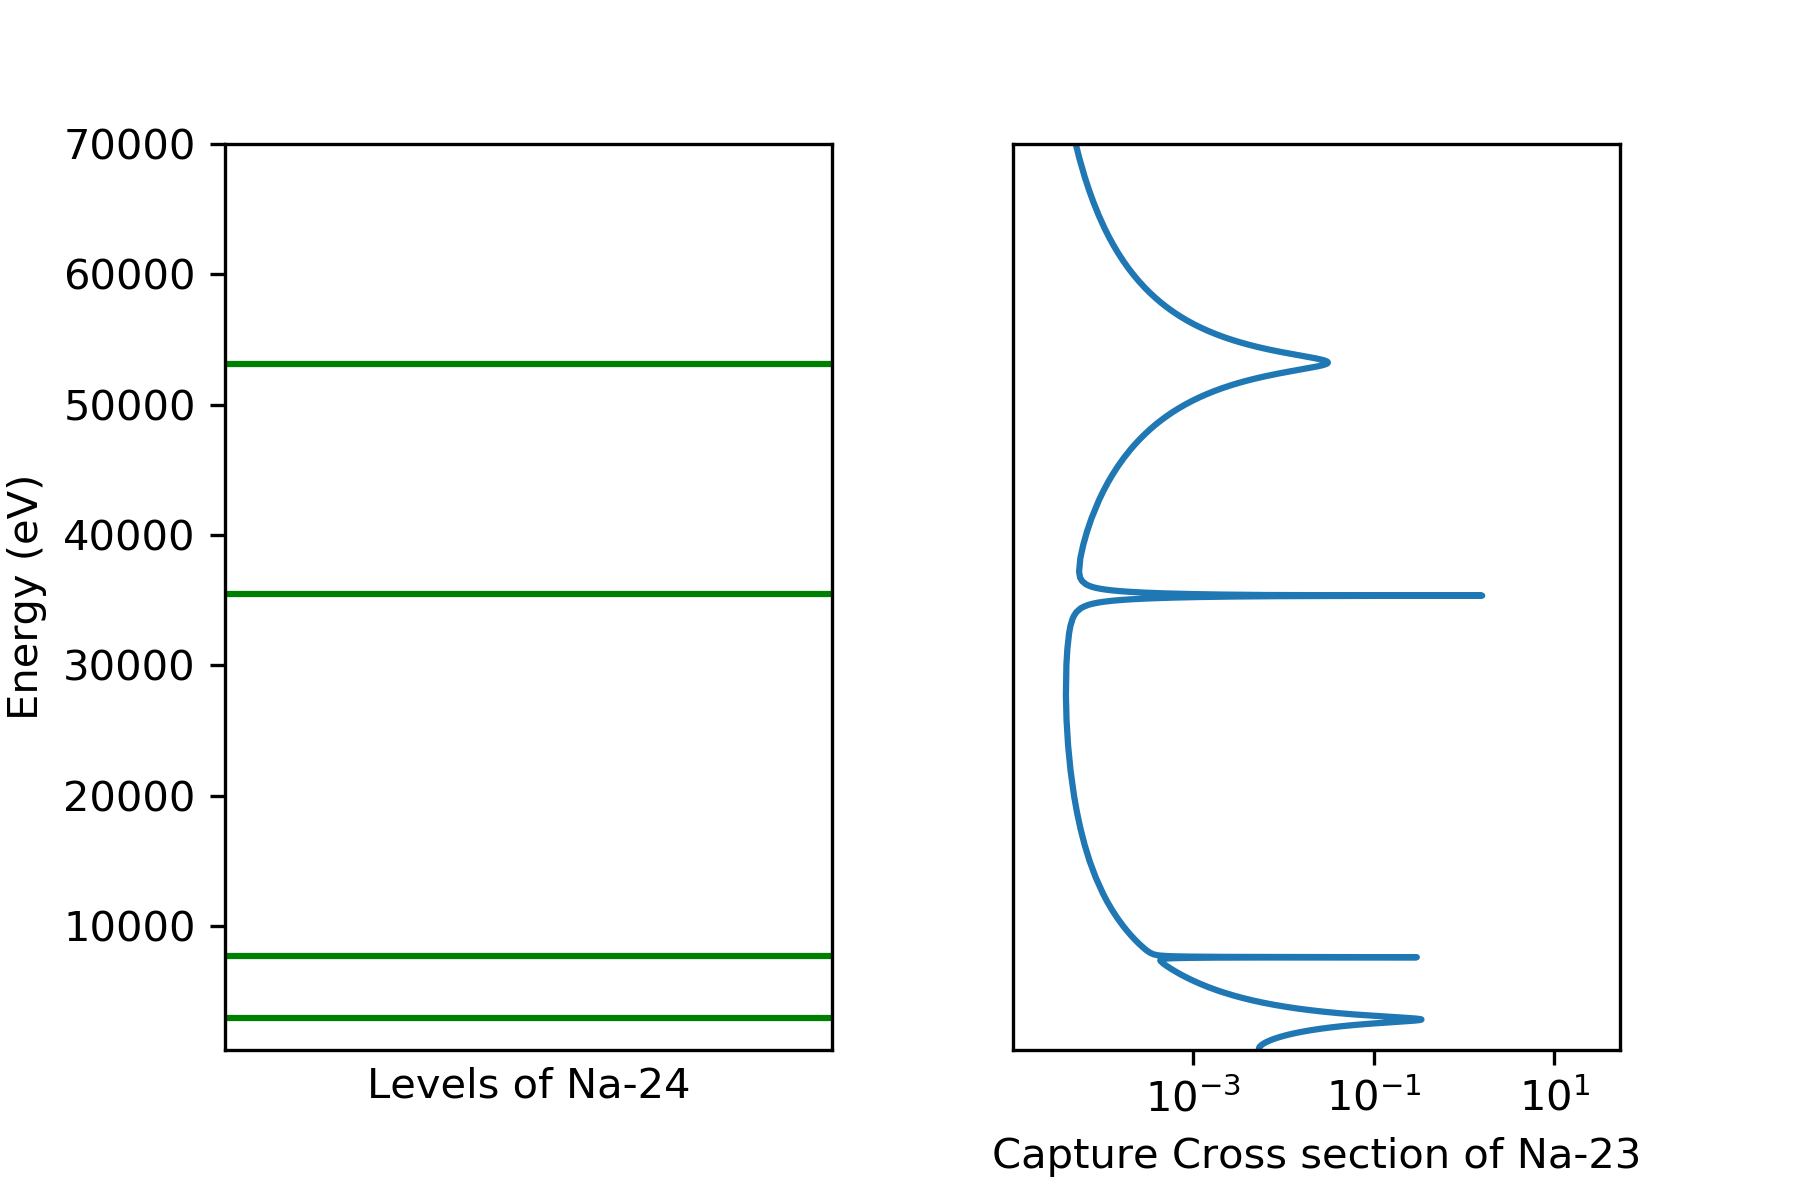
\includegraphics[scale=0.46] {figures/01-na23xs-levels.png}}\protect
\caption{\label{fig:nalevels} \footnotesize{The levels of Na-24 and the capture cross section of Na-23.}}
\end{figure}

Although the cross section of various reactions show similarities due to the shared underlying physics, the outcome and some characteristics are different, so we will review them one by one. All the reactions are summarized in Fig. \ref{fig:levels}.

Notice that the compound nucleus will have energy levels below the ground state of the target nucleus. These levels cannot be directly reached from neutron reactions, and are sometimes referred to as "negative resonances". They have some impact on the cross sections, but the discussion of this impact is well outside of the subject of this text book.

\begin{figure}[ht!]
\protect \centering{
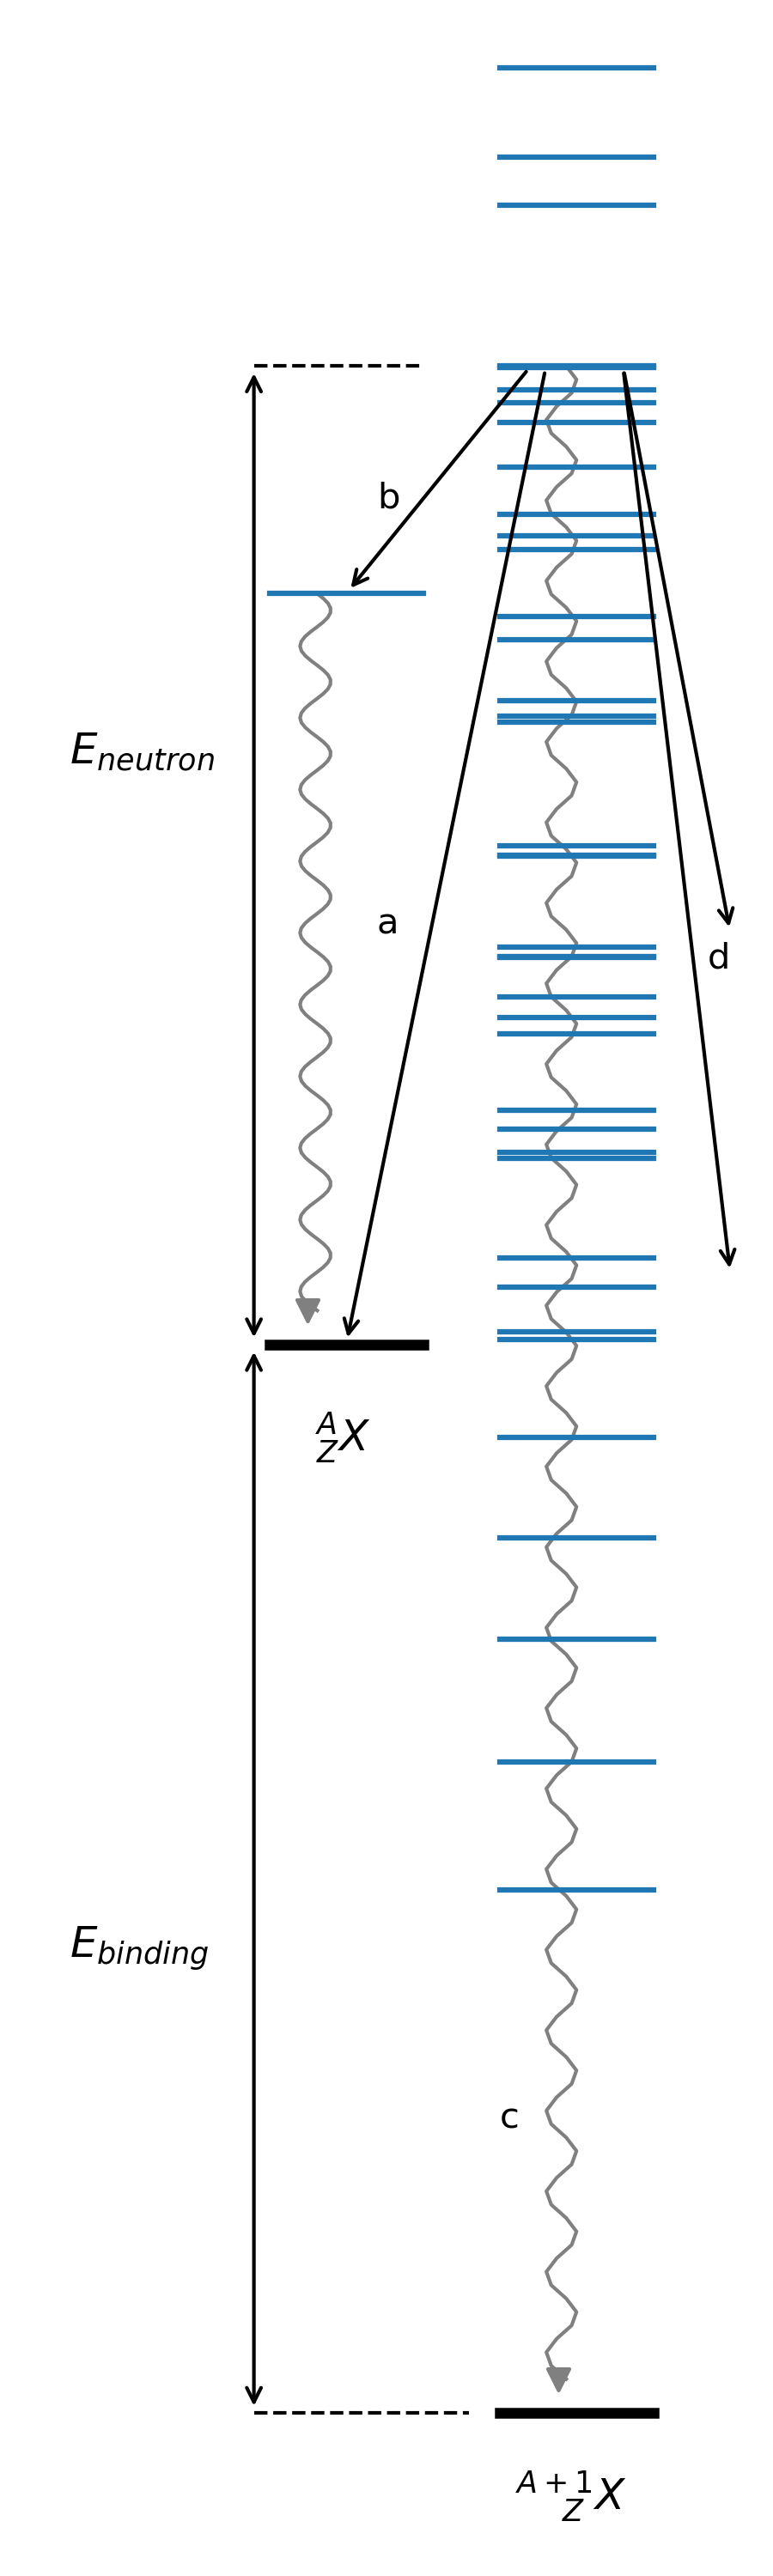
\includegraphics[scale=0.66] {figures/01-reactionlevels.png}}\protect
\caption{\label{fig:levels} \footnotesize{Schematic illustration of various reactions after compound nucleus formation. (a: elastic scattering, b: inelastic scattering, c: radiative capture, d: fission)}}
\end{figure}


\subsubsection*{Radiative capture}

In radiative capture when the CM energy of the neutron and the binding energy matches an energy level of the compound nucleus will be created in an excited state. The compound nucleus emits a cascade of $\gamma$-photons to reach the ground state (note that in Fig. \ref{fig:levels} only one $gamma$ is highlighted with a curly line, but in fact several photons can be emitted).

At low energies the energy levels of the compound nucleus are far from each other, however for higher energies, and especially for heavy nuclides, the energy levels become very dense, and it is not possible with current measurements to resolve them. This region we call unresolved resonance region (URR), which usually gives a lot of headache to nuclear reactor physicist, however at this level we will not need to worry about this. Fig. \ref{fig:u238cap} shows the capture cross section of U-238. We can observe that at lower neutron energies (below 100 eV) the single resonances can be seen, but for higher energies the resonances overlap. At even higher energies it seems that the cross section becomes suddenly smooth. At these energies the resonances are so tightly packed that they cannot be resolved experimentally at all.


\begin{figure}[ht!]
\protect \centering{
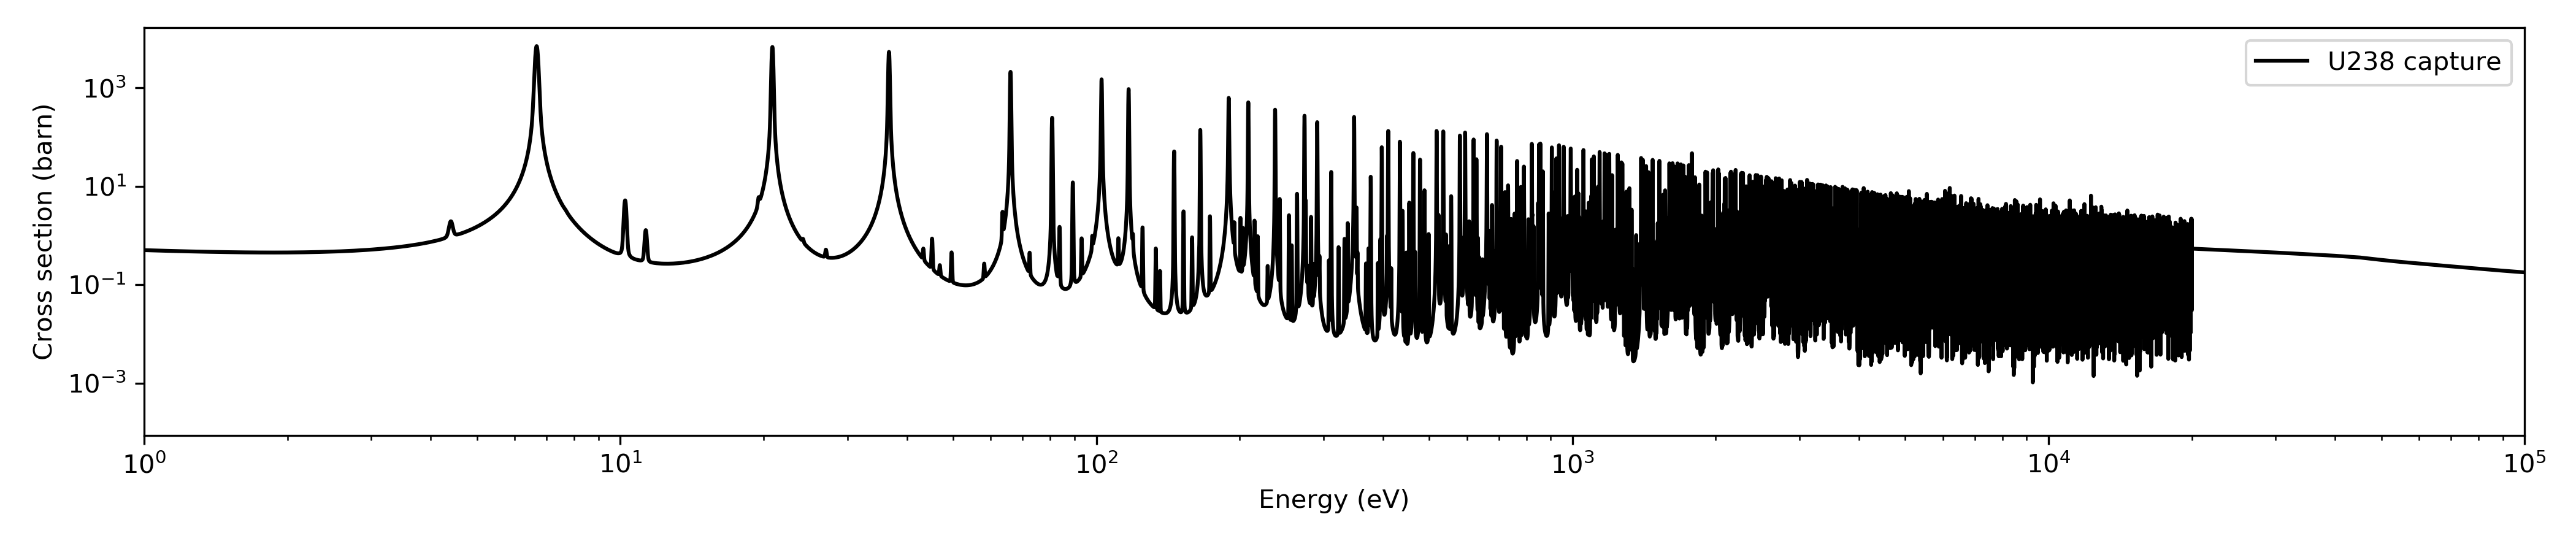
\includegraphics[scale=0.46] {figures/01-u238-capture.png}}\protect
\caption{\label{fig:u238cap} \footnotesize{Radiative capture cross section of U-238.}}
\end{figure}

One can use the Single-level Breit-Wigner (SLBW) model to describe such resonances, which will also predict that at low energies the cross section will have a $1/E^{1/2}$ or $1/v$ behavior. You can find further details on the SLBW model in the course books. This behavior can be understood phenomenologically: the slower the neutron is, the more time it spends around the nucleus, thus the higher the probability of entering a reaction. 

\subsubsection*{Fission}

In fission the excited compound state relaxes down by emitting several (most often 2-3) neutrons, and the compound nucleus splits into two (or seldom three) nuclei. 

The cross section is similar to that of the radiative capture reaction. However, as shown in Fig. \ref{fig:ufission}, some nuclides have a threshold for fission at high energies. This is due to the various size of the fission barrier. If a nuclide does not have such a threshold, and tends to undergo fission at low neutron energies as well, we call it \textit{fissile}, and nuclides which undergo fission only due to interaction with high energy (or fast) neutrons are called \textit{fissionable}.

\begin{figure}[ht!]
\protect \centering{
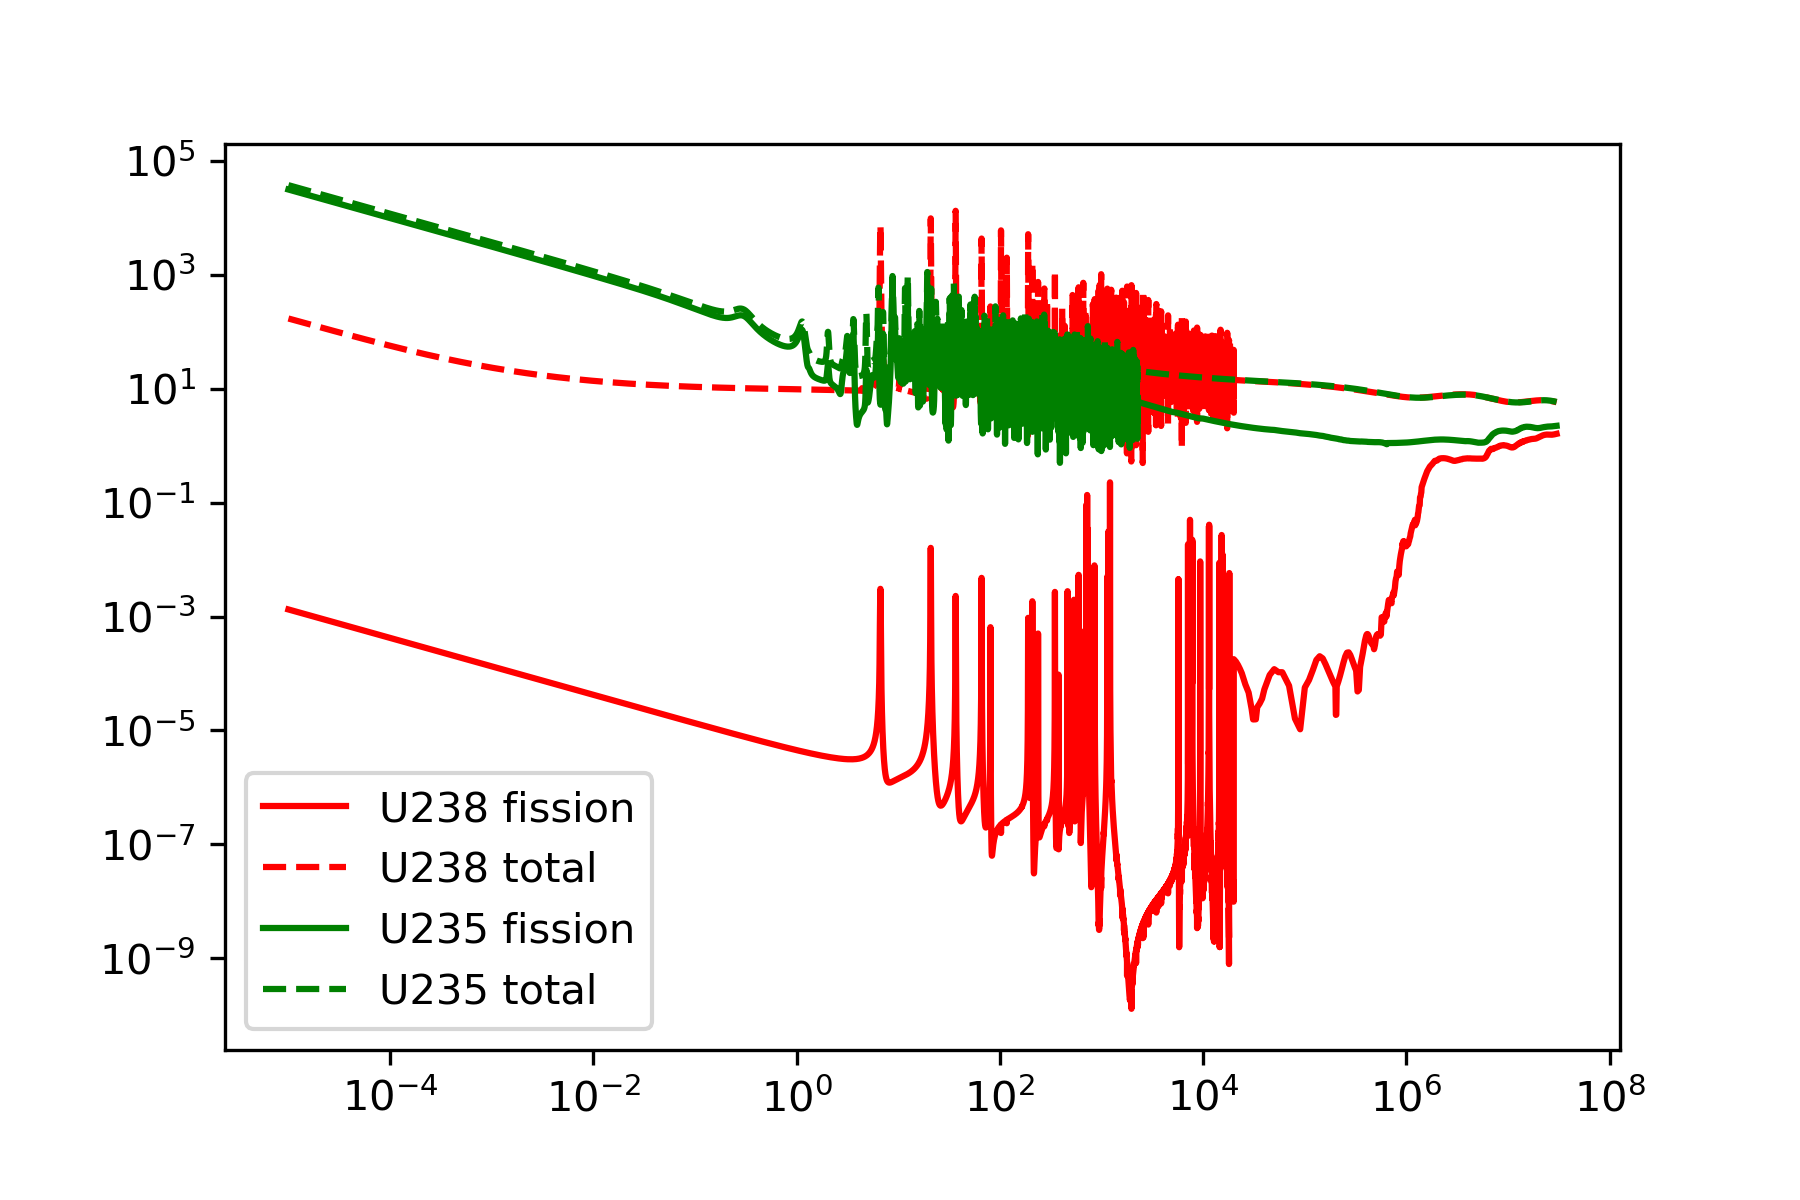
\includegraphics[scale=0.56] {figures/01-Ufission.png}}\protect
\caption{\label{fig:ufission} \footnotesize{Fission and total cross section of U-238 and U-235.}}
\end{figure}

\subsubsection*{Inelastic scattering}

In inelastic scattering the ingoing neutron is reemitted, but after after the neutron emission the target nucleus is in an excited state, therefore $\gamma$-photons are emitted to reach the ground state of the target nucleus. In such a reaction the neutron can loose a lot of energy, and the kinetic energy is not conserved. However for inelastic scattering to happen the ingoing neutron needs to have more kinetic energy than the first energy level of the target nucleus. This is shown for C-12 in Fig. \ref{fig:c12inelastic}. The threshold energy is usually several MeV, thus in typical light water reactors this reaction has little role. However for fast reactors it is often necessary to consider such reactions.

\begin{figure}[ht!]
\protect \centering{
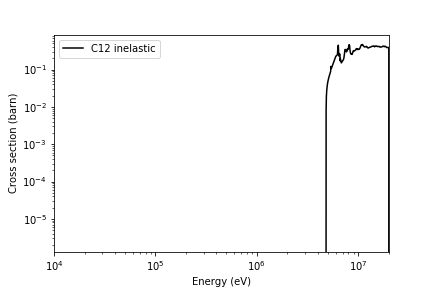
\includegraphics[scale=0.46] {figures/01-c12inelastic.png}}\protect
\caption{\label{fig:c12inelastic} \footnotesize{Inelastic scattering cross section of C-12.}}
\end{figure}

\subsubsection*{Elastic scattering}

Elastic resonance scattering happens when the compound nucleus emits a neutron, and as a result the target nucleus returns to its ground state. In this reaction the kinetic energy of the neutron is conserved. Nevertheless the cross section of such reactions is somewhat different as for the other reactions. The reason for this is that the elastic scattering cross section has three components: the previously discussed \textit{potential scattering}, the resonance scattering, and the interference scattering component. The last one is a quantum mechanical effect, and as a result the cross section may decrease before the resonance. This is shown in Fig. \ref{fig:u238elastic}.

\begin{figure}[ht!]
\protect \centering{
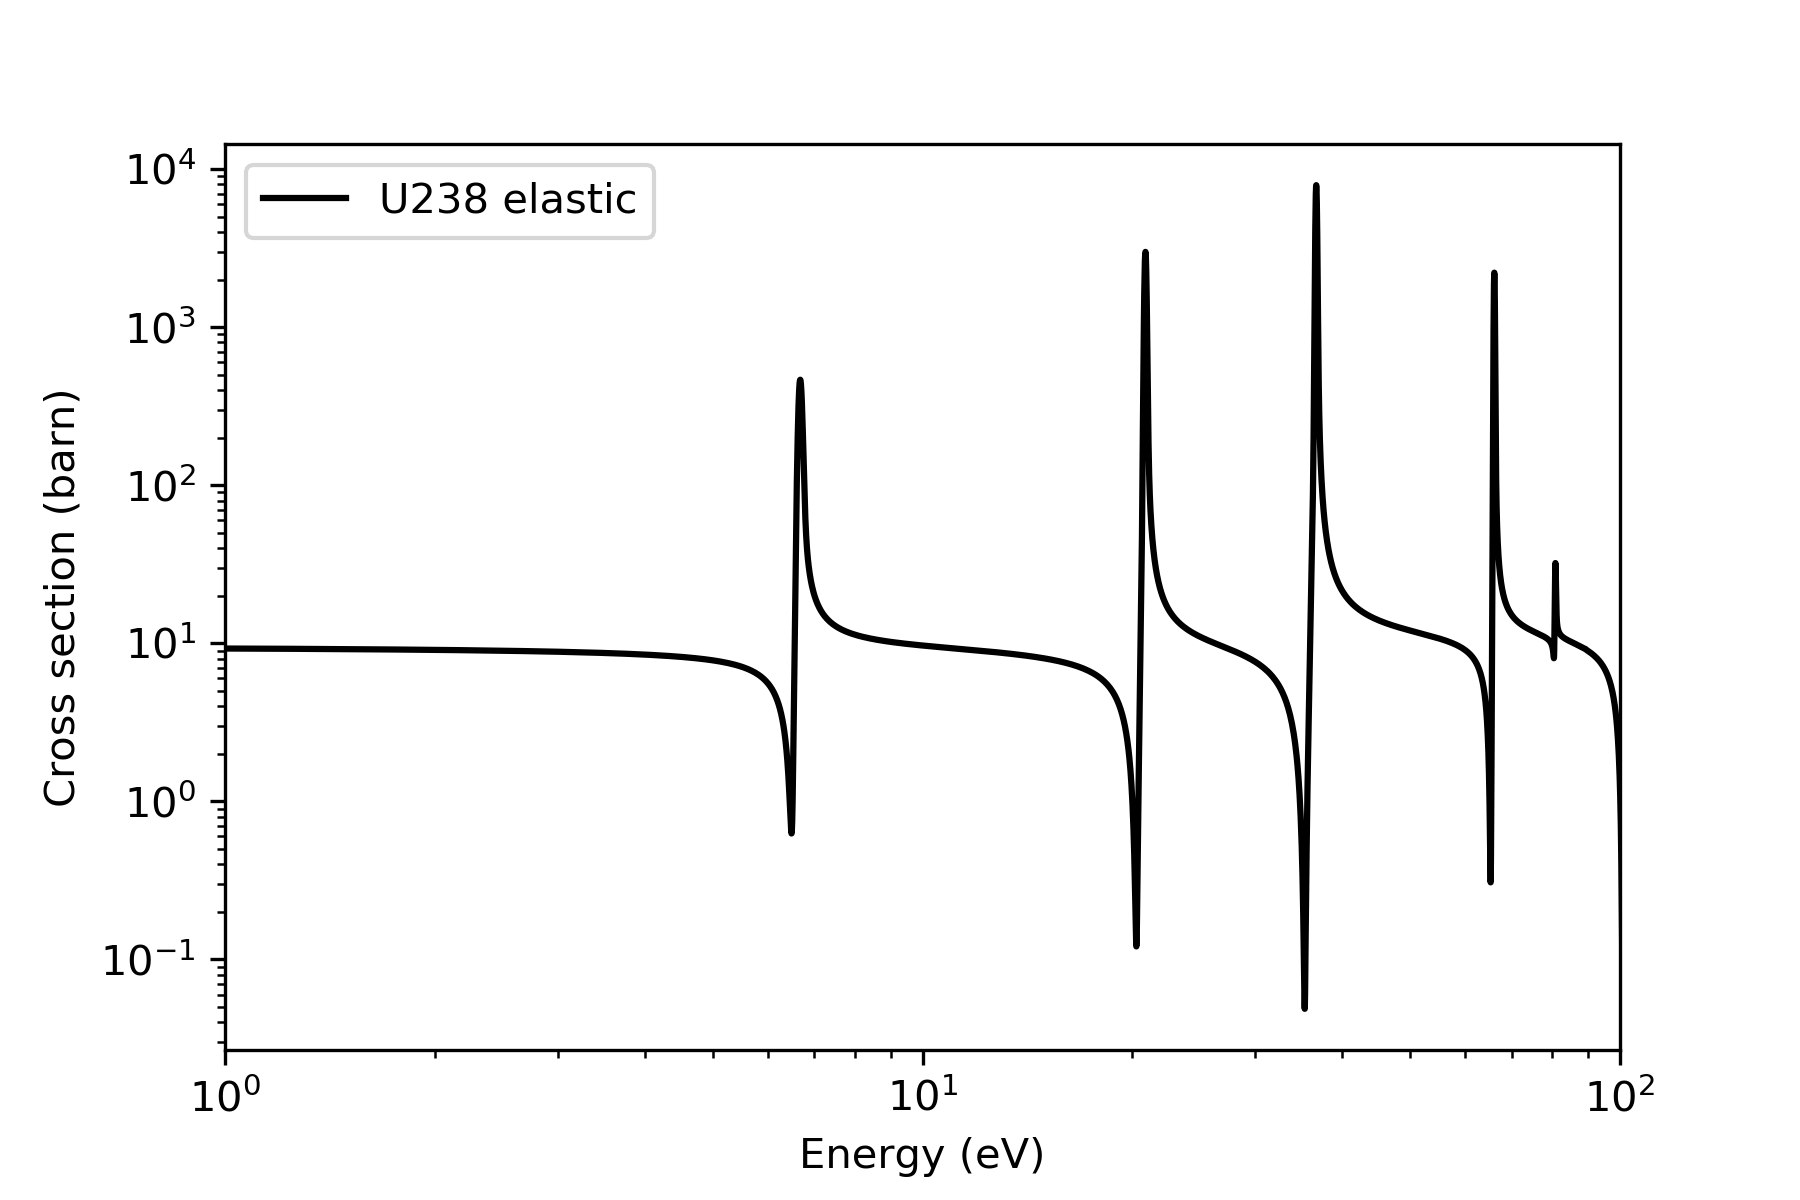
\includegraphics[scale=0.46] {figures/01-u238-resonancescatter.png}}\protect
\caption{\label{fig:u238elastic} \footnotesize{Resonances in the elastic scattering cross section of U-238.}}
\end{figure}

\subsubsection{Nuclear data libraries}

It is by now obvious that decent reactor analysis can only be done if good nuclear data is available. The various cross sections of several nuclides are measured by several laboratories, and the data is published. The standard format is called ENDF (evaluated nuclear data file), and all institutes publish the data as ENDF files. These cross sections are so called point wise cross sections: cross section evaluations at certain energies. Then the user can interpolate between the energies to obtain the cross section at any arbitrary energy. As we will see later, most of the reactor physics methods require data weighted by some function describing the energy distribution of neutrons and integrated over energy groups. This is the task of nuclear data processing tools (the most widespread code is called NJOY). Such codes can also convert the ENDF files into other formats which are then used by neutron transport codes.

There are several evaluations, which do have slight differences due to the obvious limitation of measurements. Researchers perform uncertainty studies often by executing the same calculation with various nuclear datasets. Some of the important libraries are ENDF/B-VIII.0 (from the US), JEFF-3.3 (he Joint Evaluated Fission and Fusion File). 

You can access raw ENDF files from various sources, for example the Nuclear Data Services of IAEA (\url{https://www-nds.iaea.org/} or from the Nuclear Data Center of KAERI (\url{http://atom.kaeri.re.kr/}).

Since in a recorded video lecture we will review how to access and plot these files, we will not go into further detail in this lecture note. 

\subsection{Generalization of the scattering cross section}

For scattering reactions both the energy and the direction of the particle might change. Nevertheless the value $\sigma_s(E)$ only quantifies the probability that a scattering event at neutron energy $E$ takes place. We might be however interested in the probability that the scattering results in a certain outgoing energy and direction. To describe this we can introduce differential cross sections:
\begin{itemize}
\item $\sigma_s(E\rightarrow E')$ quantifies the probability that a scattering event changes the ingoing neutron energy $E$ to $E'$ in $dE'$. Thus this cross section is in fact a distribution with unit cm$^2/$eV, and often noted with $d\sigma/dE$
\item $\sigma_s(\mathbf{\Omega}\rightarrow \mathbf{\Omega}')$ quantifies the probability that a scattering event changes the initial neutron direction $\mathbf{\Omega}$ to $\mathbf{\Omega}'$. It is often noted with $d\sigma/d\Omega$.
\end{itemize}

The name "differential cross section" is even more obvious when we consider that

$$\sigma_s(E)=\int\limits_0^\infty\sigma_s(E\rightarrow E')dE'$$

$$\sigma_s(\mathbf{\Omega})=\int\limits_{4\pi}\sigma_s(\mathbf{\Omega}\rightarrow \mathbf{\Omega}')d\mathbf{\Omega}'$$

It is however important to highlight that the dependence of $\sigma_s(\mathbf{\Omega})$ on the direction is weak, because in reactor applications the nuclei are randomly orientated within the materials. Similarly, $\sigma_s(\mathbf{\Omega}\rightarrow\mathbf{\Omega}')$ will usually not depend on the incident neutron direction, it is rather the change in the direction which is of importance, which change can be given by the cosine of the scattering angle $\theta$, which is in fact the dot product of the before and after directions $\mu_0=\mathbf{\Omega}\mathbf{\Omega}'$, therefore often one just simply uses the notation

$$\sigma_s(\mathbf{\Omega}\rightarrow \mathbf{\Omega}')=\sigma_s(\mathbf{\Omega}\mathbf{\Omega}')=\sigma_s(\mu_0)$$

By combining the differential cross sections one can define the double differential scattering cross section

$$\frac{d\sigma_s^2}{dEd\mathbf{\Omega}}=\sigma_s(E\rightarrow E',\mathbf{\Omega}\rightarrow \mathbf{\Omega}')$$

\noindent from which

$$\sigma_s(E\rightarrow E')=\int\limits_{4\pi}\sigma_s(E\rightarrow E',\mathbf{\Omega}\rightarrow \mathbf{\Omega}')d\mathbf{\Omega}'$$

$$\sigma_s(E,\mathbf{\Omega}\rightarrow \mathbf{\Omega}')=\int\limits_{0}^\infty\sigma_s(E\rightarrow E',\mathbf{\Omega}\rightarrow \mathbf{\Omega}')dE'$$

$$\sigma_s(E)=\int\limits_{4\pi}\int\limits_{0}^\infty\sigma_s(E\rightarrow E',\mathbf{\Omega}\rightarrow \mathbf{\Omega}')dE'd\mathbf{\Omega}'$$

\noindent and these concept can be generalized to the macroscopic cross sections. Analyzing and handling such data is not straightforward. However, there is one situation when the handling is not difficult: elastic potential scattering in case of isotropic scattering angle in the CM system. Some books (such as Stacey: Nuclear reactor physics) quote the relationship $\mu_c=0.07A^{2/3}E(MeV)$, which indeed is close to zero below cca 0.1 MeV for light nuclei), others (such as D\&H) quote that this is applicable for neutron energies below 1MeV for light nuclei. In this case the scattering kernel is separated as

$$\sigma_s(E\rightarrow E')=\sigma_s(E)P(E\rightarrow E')$$

\noindent where $P(E\rightarrow E')dE'$ is the probability that a neutron with initial energy $E$ will have an energy $E' \in [E',E'+dE']$. Probability density functions like these are often referred to as \textit{scattering kernels}. In the following we will investigate this probability density function for elastic scattering.

\subsection{Scattering kernel and kinematics}

As mentioned earlier, studying the kinematics of elastic neutron scattering is simpler in the center-of-mass system. The reason is that in the laboratory system the target nucleus recoils after the scattering event (due to momentum is conserved), thus the energy of the neutron get smaller with the same amount of energy what is acquired by the recoiling nucleus. However in the CoM the energies of the neutron and the nucleus is the same, and only the direction changes. 

We have earlier introduced the Center-of-Mass and Laboratory frames. Let us now further elaborate, and study the situation when a neutron elastically scatters on a target nucleus at rest (in the laboratory). Figure \ref{fig:cmlabscatter}. In the CM system, the center-of-mass is fixed, thus the target nucleus travels towards the collision. After collision the speed of the nucleus and the neutron is not changed, only the direction, the nucleus and the target travel back to back. Figure \ref{fig:cmlabrelation} shows how the two systems and the scattering angles are related to each other.

\begin{figure}[ht!]
\protect \centering{
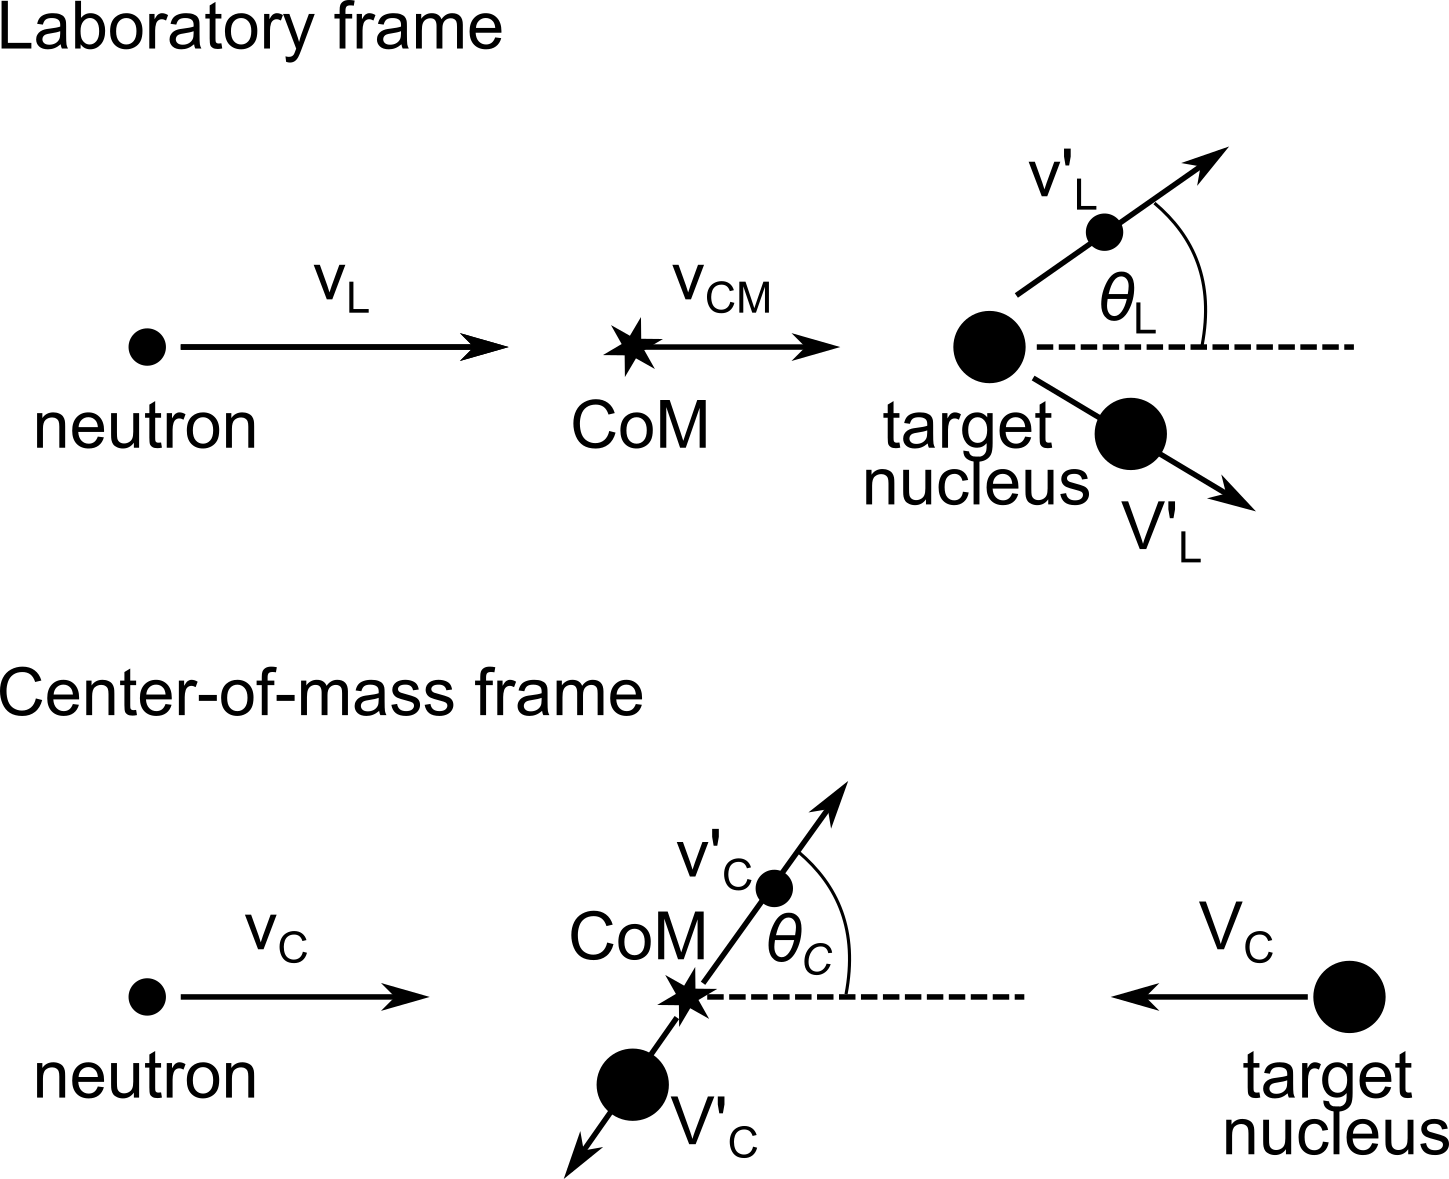
\includegraphics[scale=0.46] {figures/01-CM-LAB_scatter.png}}\protect
\caption{\label{fig:cmlabscatter} \footnotesize{Scattering in the laboratory and center-of-mass.}}
\end{figure}

\begin{figure}[ht!]
\protect \centering{
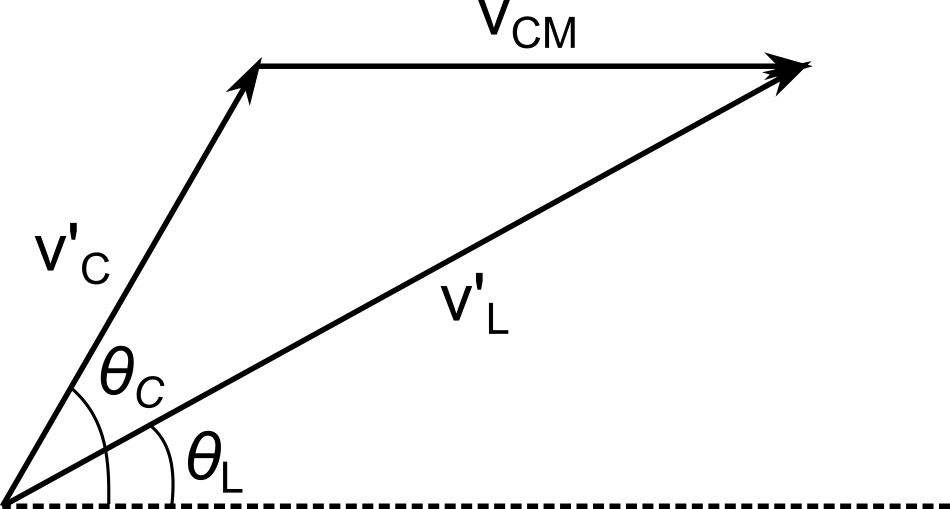
\includegraphics[scale=0.46] {figures/01-CM-LAB_relation.png}}\protect
\caption{\label{fig:cmlabrelation} \footnotesize{Relation of the laboratory and center-of-mass.}}
\end{figure}

After considering momentum and energy conservation and some elementary geometry, we can arrive to following important formula (for full derivation see D\&H p40) relating the kinetic energy in the LAB before and after the collision.

$$\frac{E'}{E}=\frac{A^2+2A\cos\theta_C+1}{(A+1)^2}$$

\noindent and by introducing 

$$\alpha=\Big(\frac{A-1}{A+1}\Big)^2$$

\noindent we can rearrange to

\begin{equation}\label{eq:muErelation}
\frac{E'}{E}=\frac{(1+\alpha)+(1-\alpha)\cos\theta_C}{2}
\end{equation}

\noindent which shows that the energy transfer from the neutron to the nucleus is directly related to the scattering angle in CM. The $\theta_C=180^\circ$ heads on collision results in a backscattered neutron with an energy $\alpha E$, thus the maximum energy the neutron can loose is $(1-\alpha)E$. In case of a hydrogen target nucleus ($\alpha=0$), the neutron can loose all its energy. However for a uranium-235 scatterer the neutron can loose only 1.7\% of its energy.

We can also see that the neutron energy after the scattering is always less than before. This however is a consequence of our assumption that the target is at rest.

Since we discovered that the scattering angle is directly related to the energy transfer, we can also presume that the probability distribution $P(E\rightarrow E')$ is directly related to the probability of scattering with an angle $\theta_C \in [\theta_C,\theta_C+d\theta_C]$. Let us use the cosine of the scattering angle $\mu_C=\cos\theta_C$ and consider that its distribution is given with $\chi(\mu_C)$. We see from Eq. \eqref{eq:muErelation} that a given $d\mu_C$ corresponds to a given $dE'$, thus 

$$P(E\rightarrow E')dE'=\chi(\mu_C)d\mu_C$$

\noindent and from  Eq. \eqref{eq:muErelation} we see that

$$d\mu_C=\frac{2dE'}{(1-\alpha)E}$$

\noindent therefore

\begin{equation}
    P(E\rightarrow E') = 
    \begin{cases}
      \frac{2\chi(\mu_C)}{(1-\alpha)E} & \text{if} \: \alpha E \leq E' \leq E \\
      0 & \text{otherwise}
    \end{cases}
\end{equation}

However, as we said before, we can safely assume below 100 keV that scattering is isotropic in the CM frame. In that case, the cosine $\mu_C$ is uniformly distributed between $[-1,1]$, therefore

$$\chi(\mu_C)=\frac{1}{2}$$

\noindent and with that the scattering kernel is

\begin{equation}
    P(E\rightarrow E') = 
    \begin{cases}
      \frac{1}{(1-\alpha)E} & \text{if} \: \alpha E \leq E' \leq E \\
      0 & \text{otherwise}
    \end{cases}
\end{equation}

\noindent which means that the outgoing energy is also uniformly distributed between $[\alpha E, E]$ as shown in Figure \ref{fig:isotroppdf}. With this the differential scattering cross section of elastic scattering becomes.

\begin{equation}
    \sigma_s(E\rightarrow E') = 
    \begin{cases}
      \frac{\sigma_s(E)}{(1-\alpha)E} & \text{if} \: \alpha E \leq E' \leq E \\
      0 & \text{otherwise}
    \end{cases}
\end{equation}

\noindent and as we so before the potential scattering cross section is only weakly dependent on the energy.

\begin{figure}[ht!]
\protect \centering{
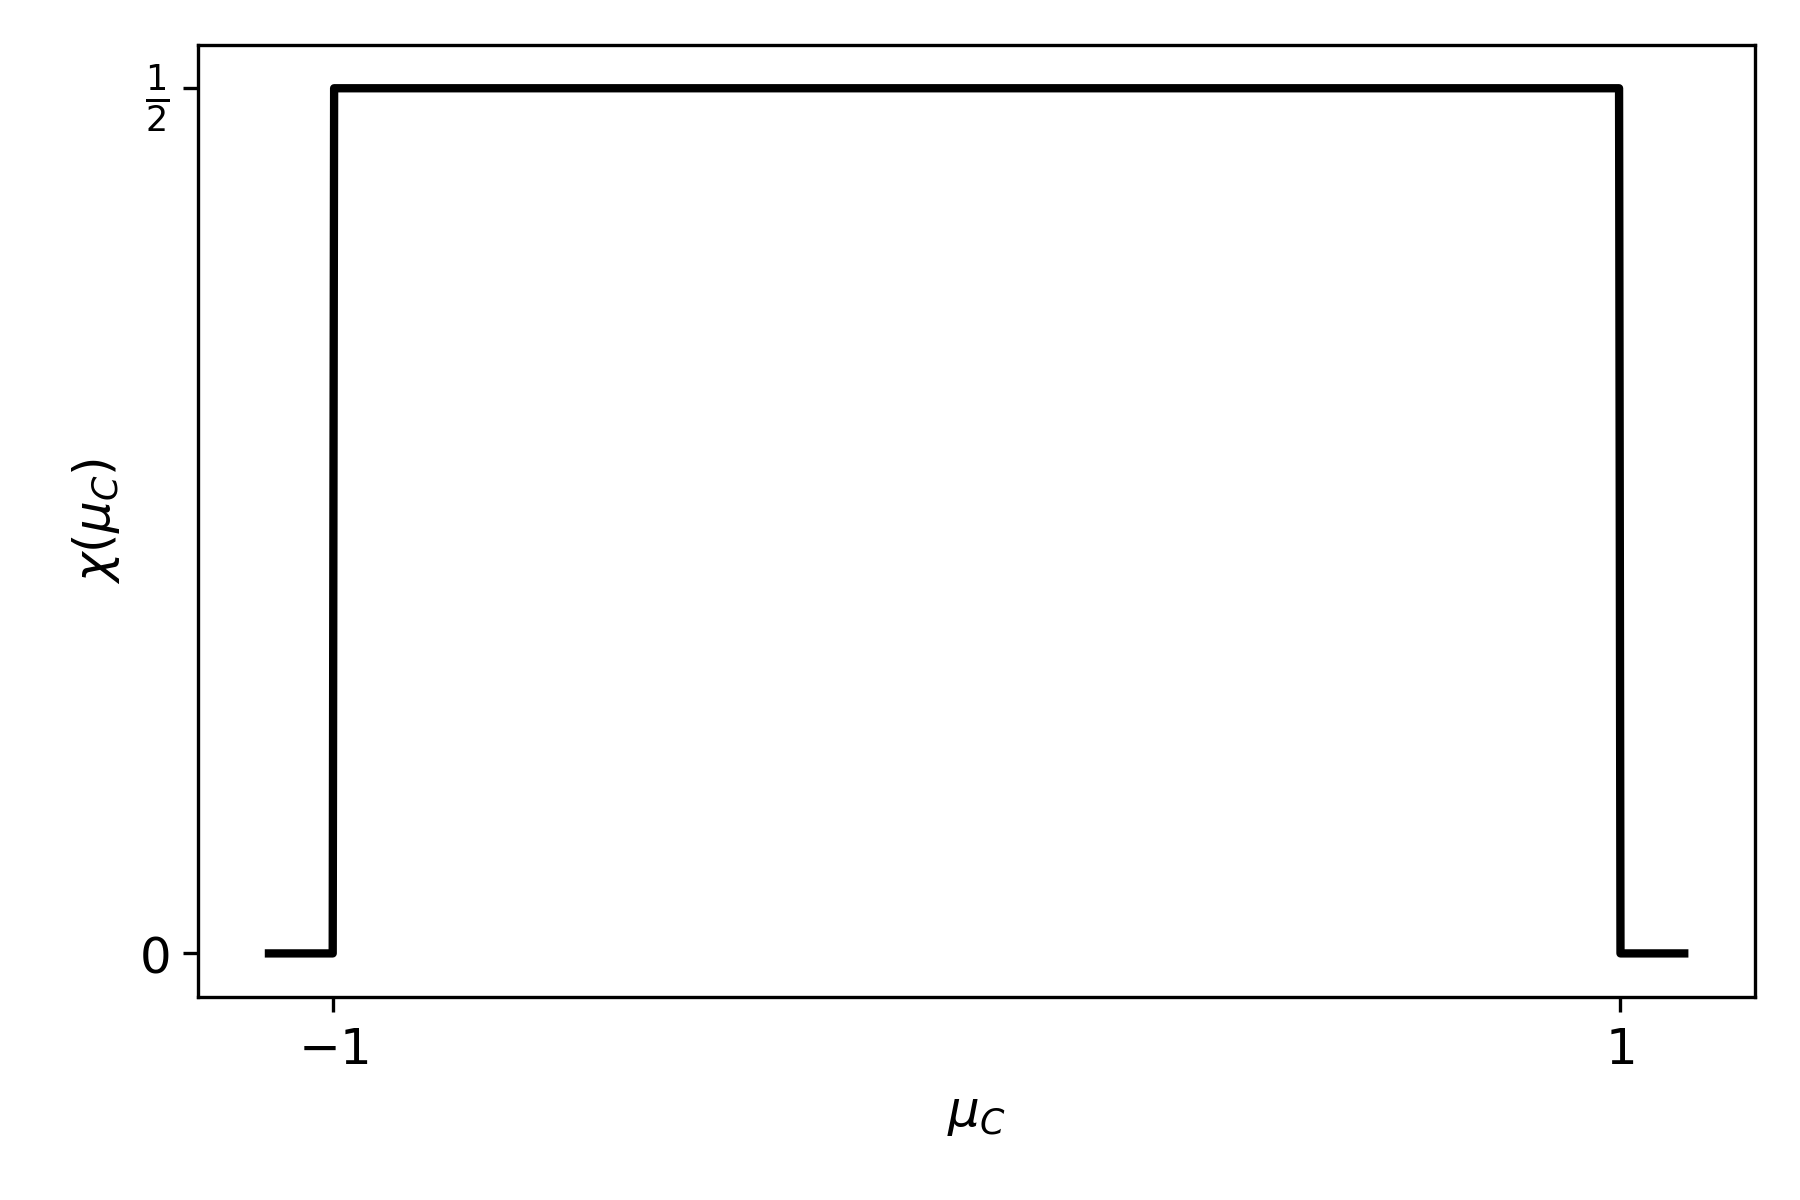
\includegraphics[scale=0.43] {figures/01-isotropmucpdf.png}
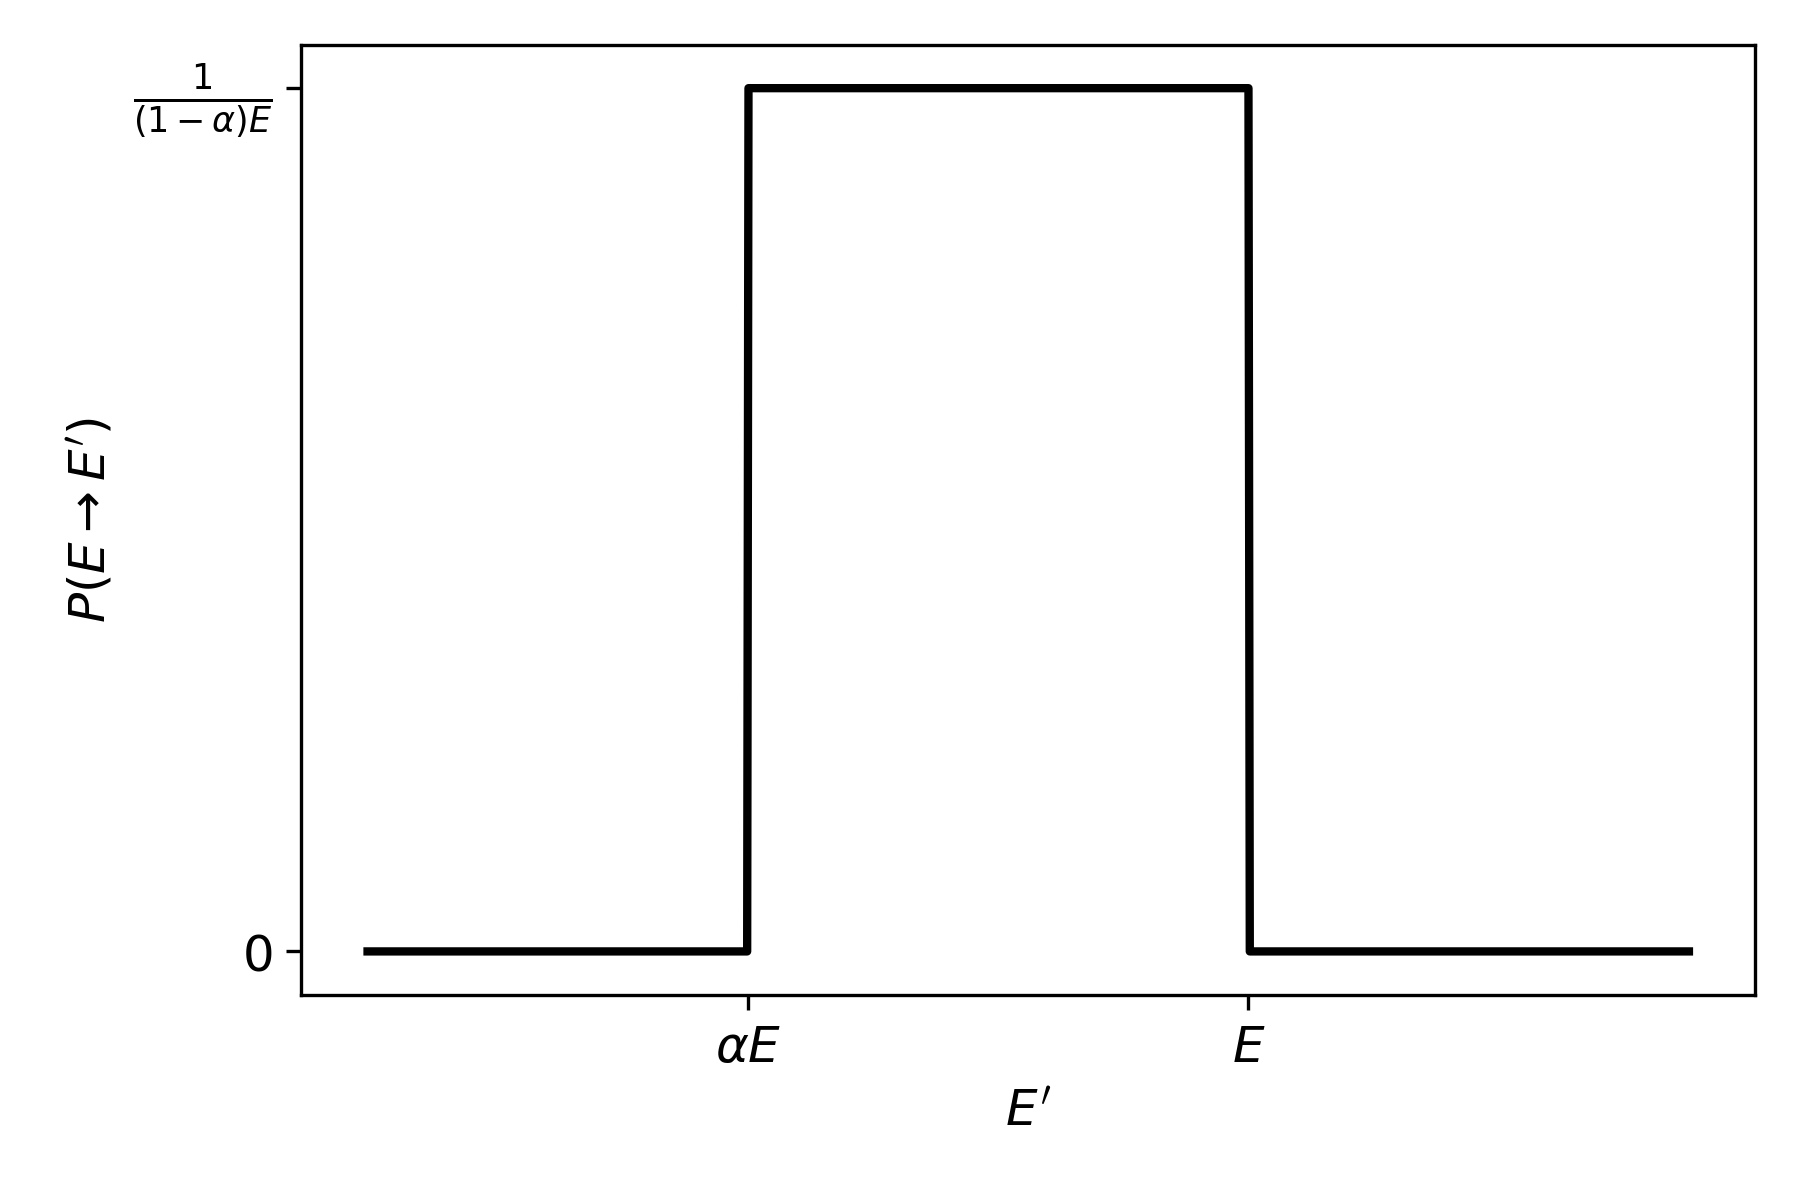
\includegraphics[scale=0.43] {figures/01-elastickernelpdf.png}}\protect
\caption{\label{fig:isotroppdf} \footnotesize{Illustration of $\chi(\mu_C)$ and $P(E\rightarrow E')$.}}
\end{figure}

Within this course we will not handle the case when elastic scattering is not isotropic in the CM. Nevertheless, as said before most often the assumption of isotropy in CM is valid at the neutron energies encountered in light water reactors. 

As we saw earlier, in fissile material the probability of fission events is much higher with low energy neutrons than with fast neutrons. Therefore, elastic scattering plays an important role in slowing down neutrons to thermal energies also materials which efficiently slow neutrons down as we will discuss in more detail in later sections. We refer to such materials as \textit{moderator}. In a light water reactor, the coolant water act as the moderator. Also, one needs to highlight again is that the energy lost by the neutron will recoil the scatterer nucleus, which leads to radiation damage. Therefore, the recoil energy is important for damage studies, although it plays little role for reactor physics.

It is also important to note that from our previous discussions we can relate the scattering angles in the CM and LAB frames by

$$\theta_L=\tan^{-1}\Big(\frac{\sin \theta_C}{\frac{1}{A}+\mu_C}\Big)$$

\noindent or as it is given in some books

$$\mu_L=\frac{A\mu_C+1}{\sqrt{A^2+2A\mu_C+1}}$$

\noindent which can be used to calculate the average scattering cosine in the LAB:

$$\bar{\mu}_L=\frac{1}{2}\int\limits_{-1}^{1}\frac{A\mu_C+1}{\sqrt{A^2+2A\mu_C+1}}d\mu_C=\frac{2}{3A}$$

\noindent which means that scattering is not isotropic in the LAB frame for light nuclei. As the mass number $A$ increases, the average cosine is converging to 0. This is important to remember, since one often only remembers that scattering is isotropic, but tends to forget that only in the CM frame. As we will see later, this will be one of the main limitations for applying diffusion theorem for the movement of neutrons, since diffusion is based on the assumption that scattering is isotropic in the LAB.


\subsection{Effects of nuclear motion}

Up to this point we have always assumed that the target is at rest. However, due to thermal motion this is not the case, nevertheless the speed of thermal motion is usually negligible compared to the neutron speed. However when the neutron energy is comparable to the thermal energy ($kT$) we need to take into account effects due to thermal motion. Neutrons having such low energies are referred to as \textit{thermal neutrons}. Typically then the neutron energy is below 1 eV.

An other important occasion when thermal motion plays a role is at resonances. A resonance has a width often less then 1 eV, therefore if slight thermal motion can have an effect on the energy dependence of the cross section around the resonance (even if the resonance occurs above thermal energies). This is called Doppler effect. 

In this text we will not derive the formalism of nuclear motion, because it is rather tedious, and the conclusions are more interesting than the way how we reached it. Proper derivations can be found in D\&H p45. The starting point of these derivations is that when calculating the interaction frequency we have to take into account the relative speed between the neutron and the nucleus:

\begin{equation}
|\textbf{v}-\textbf{V}|\sigma(|\textbf{v}-\textbf{V}|)N
\end{equation}

\noindent where the neutron moves with velocity $\textbf{v}$ and the nucleus moves with velocity $\textbf{V}$. Then in the next step one needs to acknowledge, that not all nuclei move with the same velocity, instead one needs to take into account a distribution for the nucleus velocity and at the end one can arrive to a thermally averaged cross section. If that is then applied on  resonances one could observe the behavior illustrated in Figure \ref{fig:doppler}: the resonance broadens while its peak decreases with increasing temperature. Therefore this is often called Doppler-broadening. As we will see, later, although the integral under the resonance is unchanged due to increasing temperature, still the probability of neutrons being absorbed by the resonance increases, because while neutrons loose their energy there is an increasing probability that they encounter the nucleus at the resonance energy. Therefore Doppler-broadening has an important safety implication: with increasing temperatures the number of neutrons (therefore the power) decreases.

\begin{figure}[ht!]
\protect \centering{
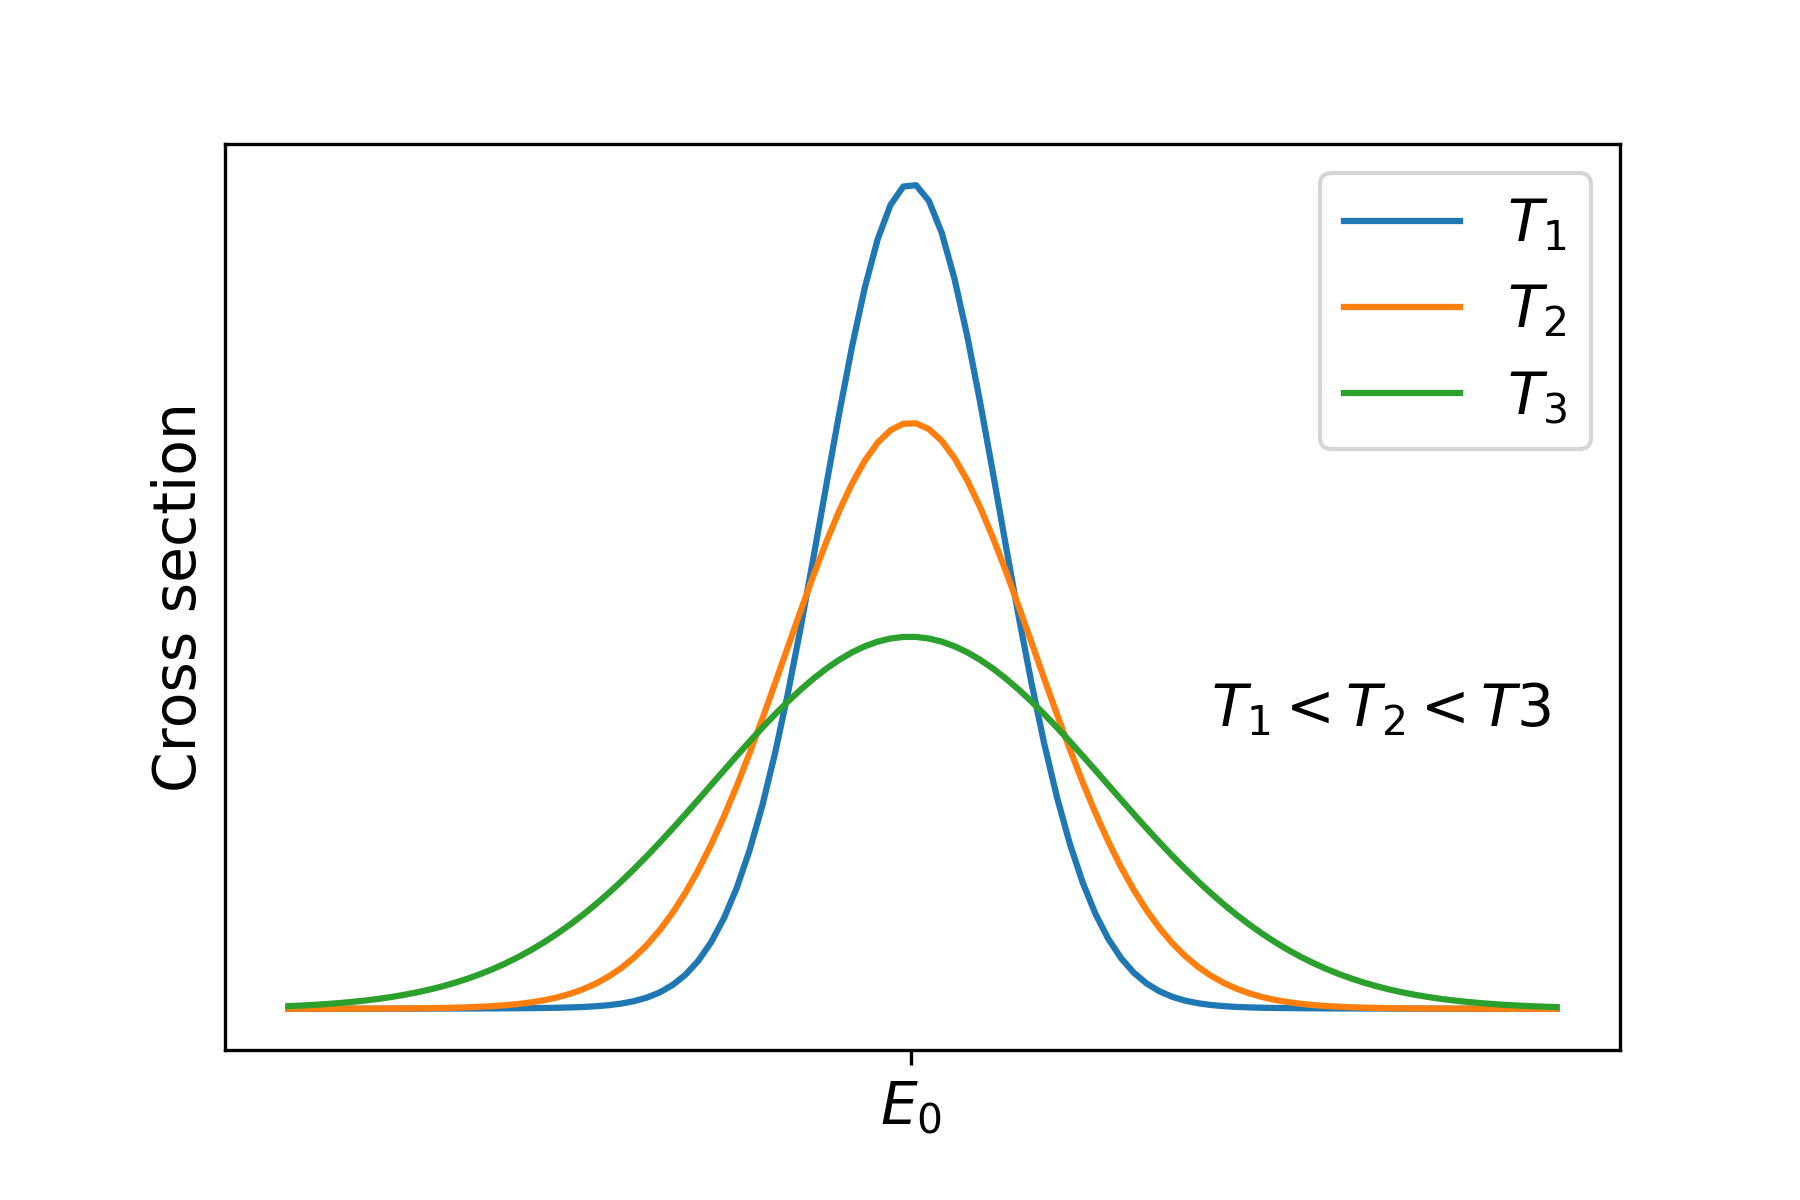
\includegraphics[scale=0.46] {figures/01-doppler.png}}\protect
\caption{\label{fig:doppler} \footnotesize{Doppler broadening of resonances.}}
\end{figure}

Another noteworthy impact of nuclear motion is for the differential scattering cross section. The derivation of such scattering kernel is an enormous task, the interested reader can find joy in reading M. M. R. Williams:  The Slowing Down and Thermalization of Neutrons (freely available from OECD NEA). For us now again mostly the conclusion, illustrated in Figure \ref{fig:thermalkernel} is of interest. At thermal energies, the neutron in fact can gain energy from a scattering event. This is called \textit{upscattering}. We can see that with increasing the energy of the incoming neutron the scattering kernel becomes the uniform distribution we have derived before, however for lower energy neutrons upscattering is more and more probable. Such scattering kernel can be given as


\begin{equation}
\begin{aligned}
\sigma_s(E'\rightarrow E)=\frac{\sigma_s}{2E'}\eta^2\Bigg[\text{erf}\Bigg(\eta\sqrt{\frac{E}{kT}}-\rho\sqrt{\frac{E'}{kT}}\Bigg)\pm \text{erf}\Bigg(\eta\sqrt{\frac{E}{kT}}+\rho\sqrt{\frac{E'}{kT}}\Bigg)\Bigg]+ \\ \frac{\sigma_s}{2E'}\eta^2\exp\Bigg(-\frac{E-E'}{kT}\Bigg)\Bigg[\text{erf}\Bigg(\eta\sqrt{\frac{E'}{kT}}-\rho\sqrt{\frac{E}{kT}}\Bigg)\mp \text{erf}\Bigg(\eta\sqrt{\frac{E'}{kT}}+\rho\sqrt{\frac{E}{kT}}\Bigg)\Bigg]
\end{aligned}
\end{equation}

\noindent where

\[
\eta=\frac{A+1}{2\sqrt{A}} \quad \text{and} \quad \rho=\frac{A-1}{2\sqrt{A}}
\]

\noindent and the upper sign is for $E\leq E'$, and the lower sign is for $E\geq E'$.

\begin{figure}[ht!]
\protect \centering{
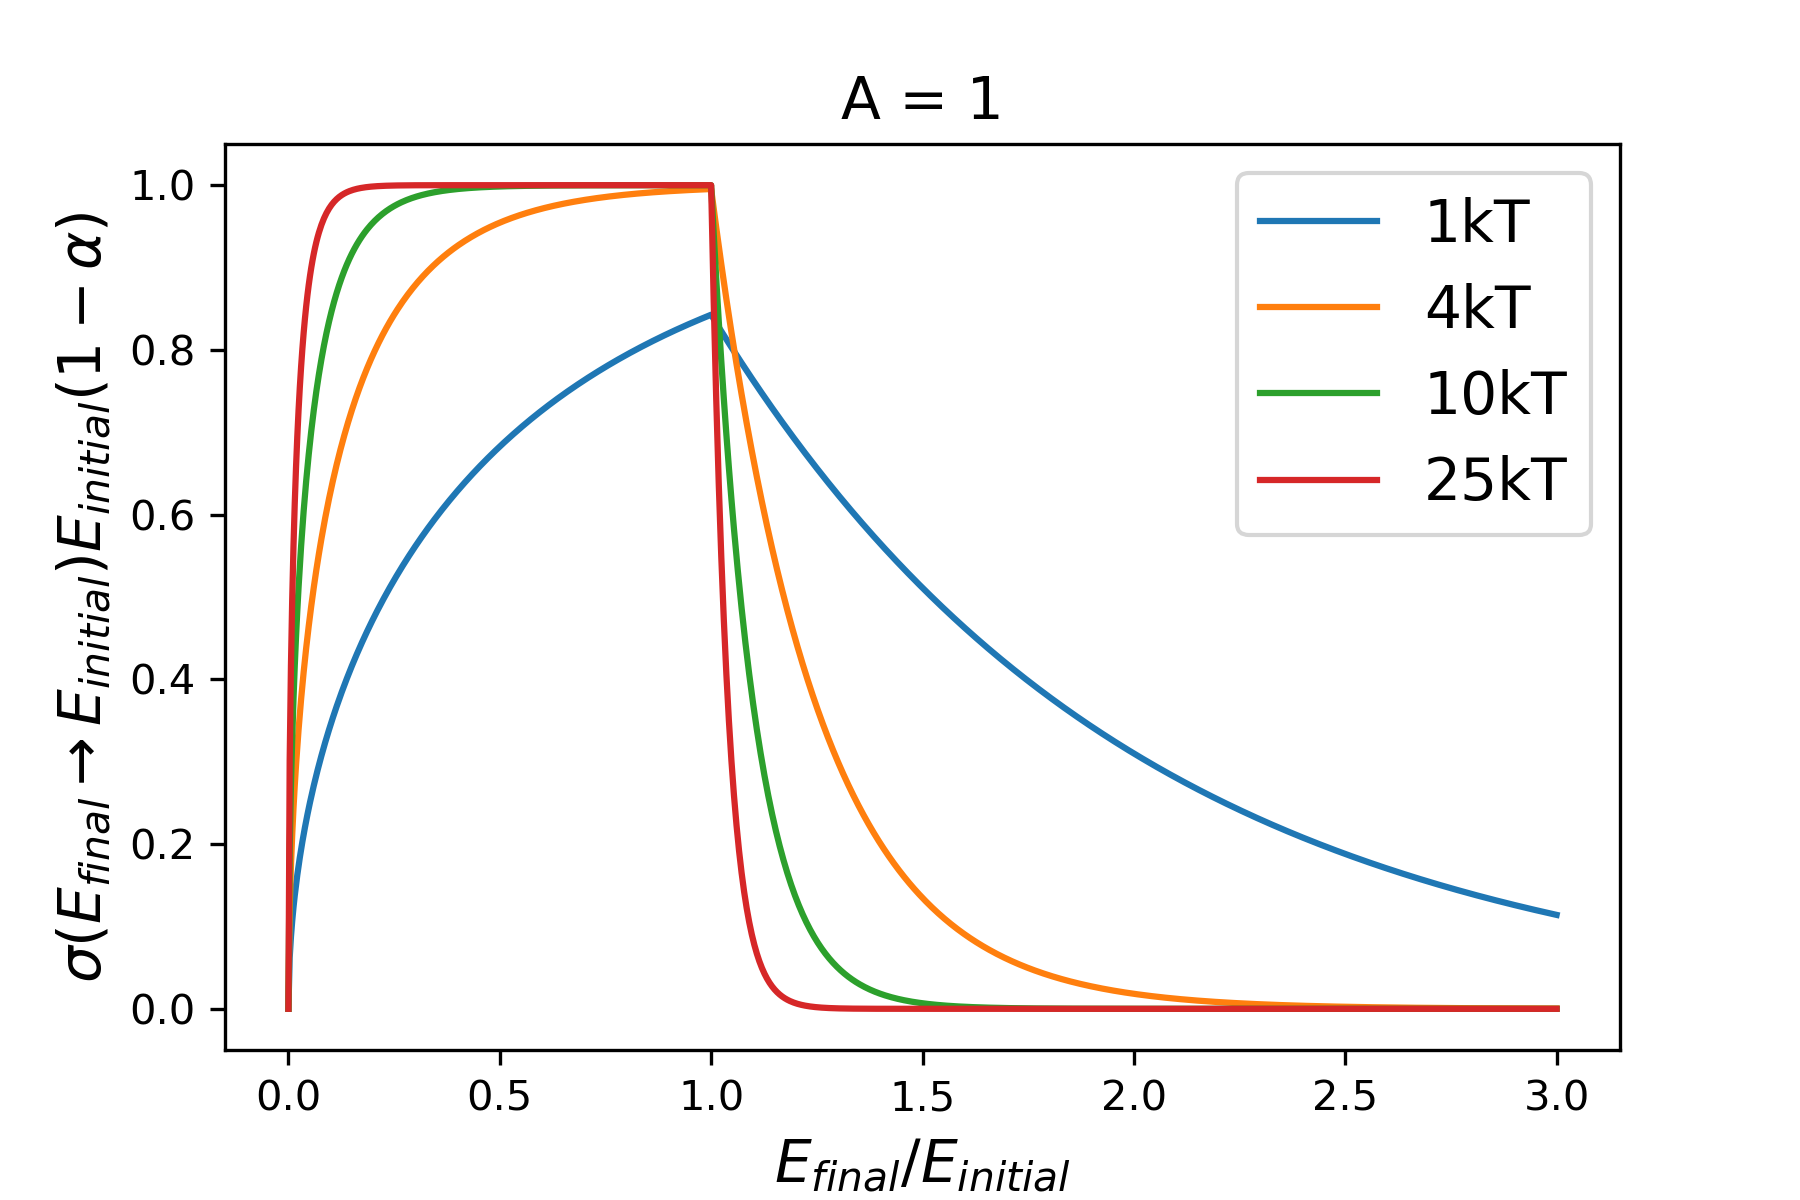
\includegraphics[scale=0.46] {figures/01-thermalscatteringkernel1.png}
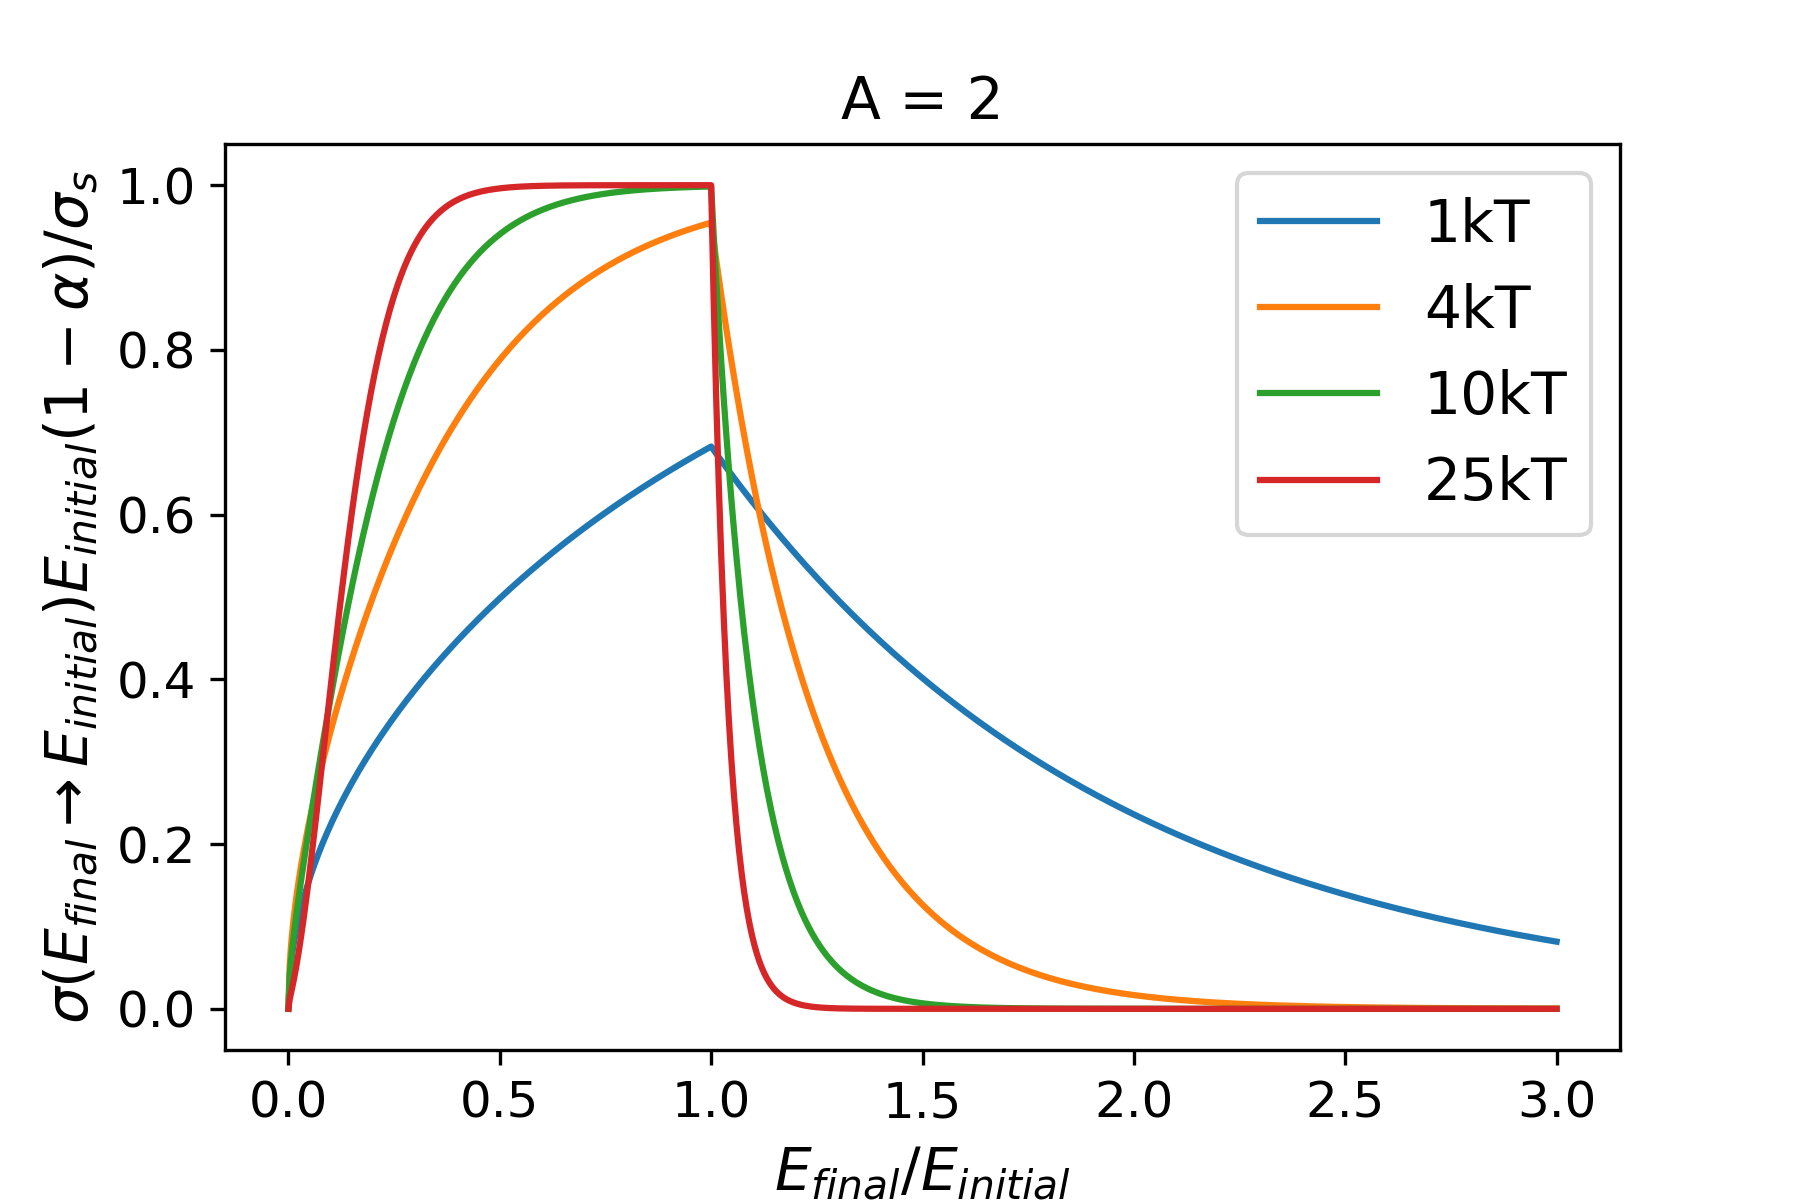
\includegraphics[scale=0.46] {figures/01-thermalscatteringkernel2.png}
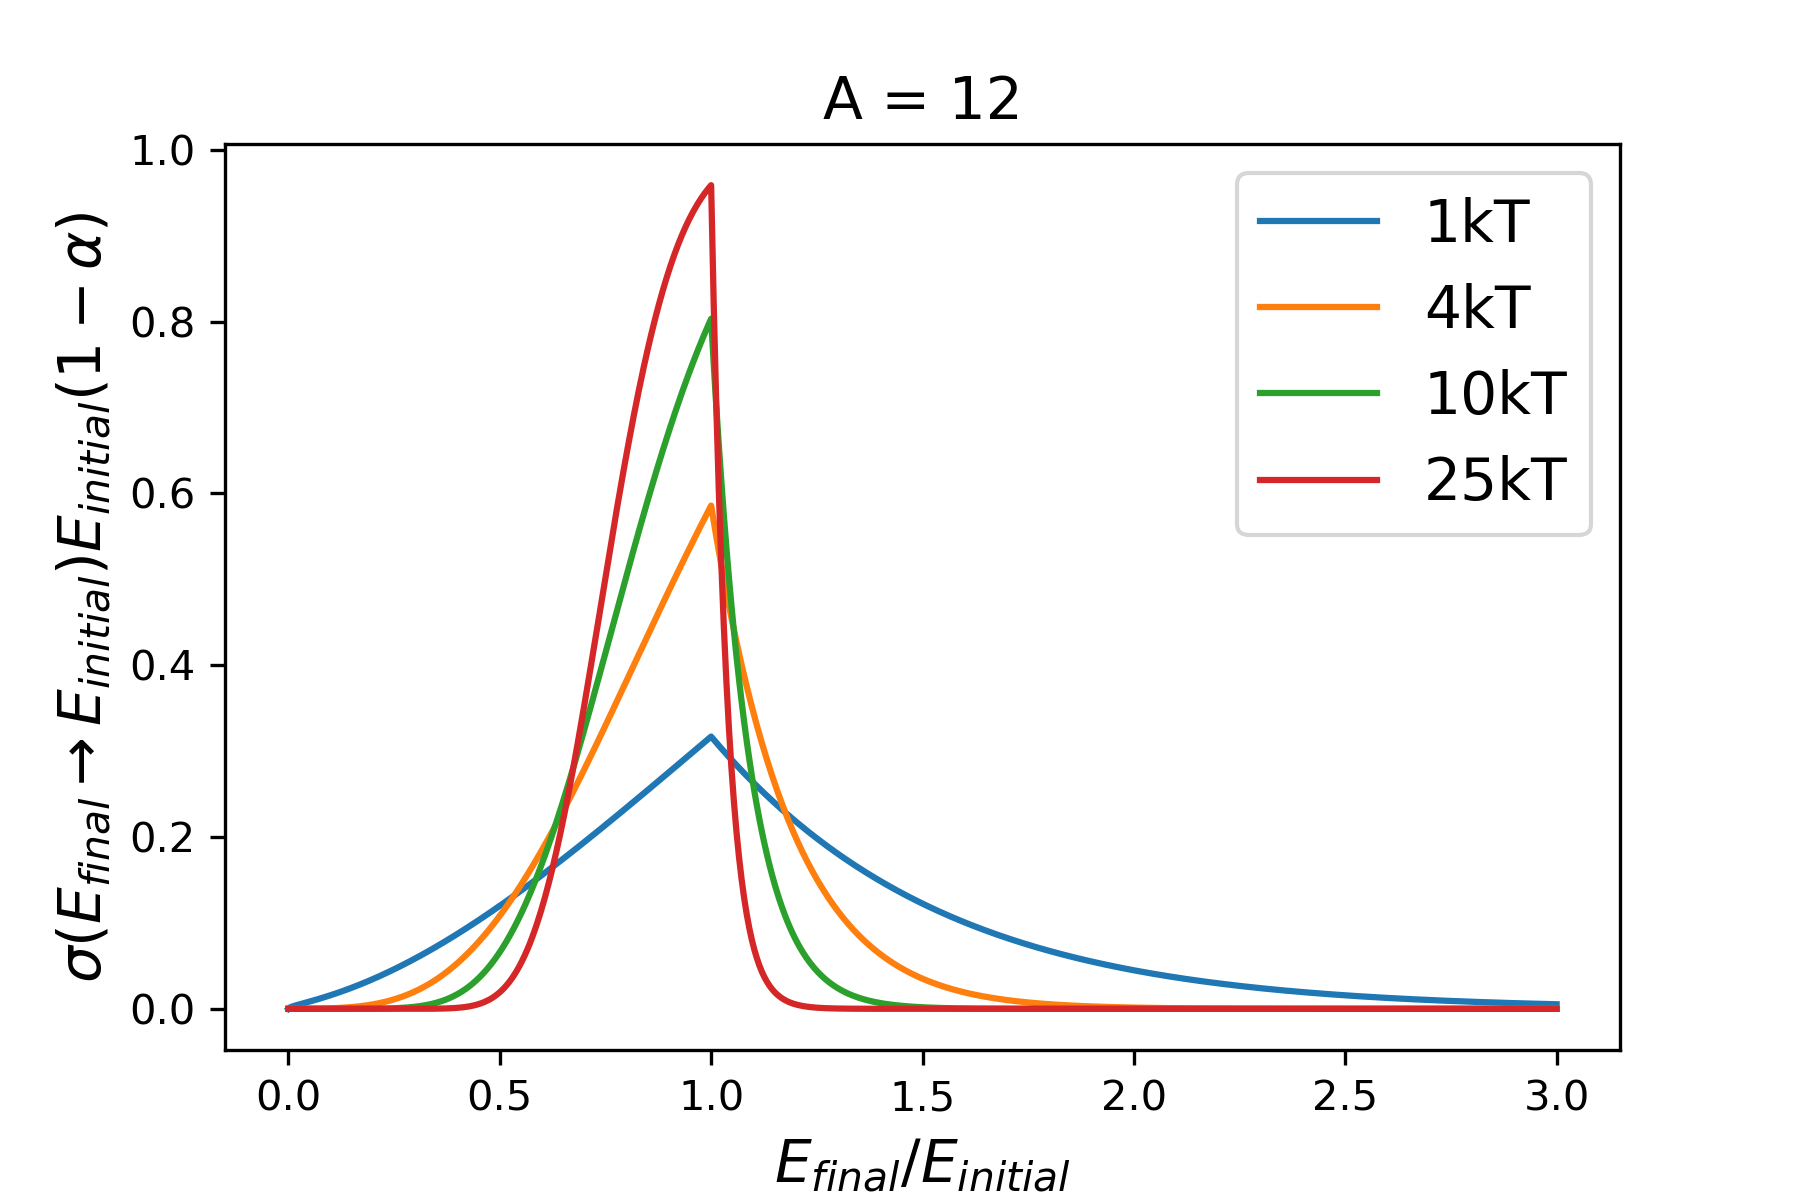
\includegraphics[scale=0.46] {figures/01-thermalscatteringkernel12.png}}\protect
\caption{\label{fig:thermalkernel} \footnotesize{Thermal scattering kernel.}}
\end{figure}

\subsection{Impact of molecular bounds}

Without going into details, it has to be mentioned that chemical bounds and crystal structures also influence scattering kinematics of thermal neutrons. This is relevant in reactor physics, since the scattering hydrogen atoms are bounded in water, which is used as the coolant and moderator of LWRs. Usually special tables are created and used that account for thermal binding effects. These are called $S(\alpha,\beta)$ tables. The theory behind the $S(\alpha,\beta)$ formalism roots in quantum mechanics, and the previously mentioned book of Williams provides a more detailed description for the interested reader. The only implication for us will be that in Monte Carlo calculations we will need to link to such tables when including materials like water in our problem.


\subsection{Nuclear fission}

Fig. \ref{fig:binding} shows that the average binding energy per nucleon has a maximum at Ni-62. Therefore fusing lighter nuclei or splitting (fissioning) heavier nuclei can lead to tighter bound nuclei, and the difference of binding energy is released in the form of energy. The main goal of building nuclear reactors is to extract the energy released during the fissioning of heavy nuclei. The reason that heavier nuclei undergo fission spontaneously only with a low probability is that the short range nuclear forces give rise to a potential energy barrier (or fission barrier), which usually has a height of 6-9 MeV. 

In order to overcome this barrier first some energy needs to be supplied to the nucleus:

\begin{enumerate}
\item by an energetic particle, for example a $\gamma$ photon (photofission)
\item by capturing a neutron to cover the energy with the binding energy of the neutron
\item by combining 1. and 2.: capturing a fast neutron
\item seldom fission can happen due to quantum mechanical tunneling (spontaneous fission)
\end{enumerate}

Nuclides which can fission by capturing slow neutrons are called \textit{fissile} (eg. U235, Pu239), wheras nuclices which have too high fission barriers therefore undergo fission only with fast neutrons are called \textit{fissionable} (eg. U238, Pu240). Recall, that for these nuclides the fission cross section presets a threshold energy, below which the probability of fission is almost negligible and the cross section is several orders of magnitude lower (eg. the fission cross section of U-238 in Fig. \ref{fig:ufission}).

It is however possible that after the neutron absorption of a nuclide the compound nucleus decays to its ground state, thus the neutron is lost for the chain reaction. The relative balance of capture and fission can be described by the 

\begin{equation}
\textit{capture-to-fission ration}=\frac{\sigma_c}{\sigma_f}
\end{equation}

of a given nuclide. This ratio of course does depend on the energy of the incoming neutron.

A typical fission reaction look as 

\[
n+{}_{92}^{235}U\rightarrow {}_{92}^{236}U^* \rightarrow \text{fission reaction products}
\]

where the reaction products cover a wide variety of particles and carry cca 200 MeV energy:

\begin{itemize}
\item charged and energetic fission products (nuclei with medium mass number), which quickly slow down in the surrounding media (while picking up electrons), and loosing their energy.
\item several neutrons with large kinetic energy
\item $\gamma$ photons
\item $\beta$ particles and neutrinos from the decay of fission products
\end{itemize}

The fission products has a distribution given by the fission yield (ie. probability) of the nuclide created in fission. In fission the nucleus is usually split asymmetrically, therefore the fission yield curve has two distinct peaks as shown in Fig. \ref{fig:fissyield}. With lower probability the nucleus can split into three fission products (ternary fission), when a third, light nuclide (eg. H-3) is created. In the top figure we can see a small "island" of light nuclides which are the result of ternary fission. The fission yield depends both on the ingoing neutron energy (and is usually tabulated separately for thermal and for fast neutrons) and on the target nuclide.

\begin{figure}[ht!]
\protect \centering{
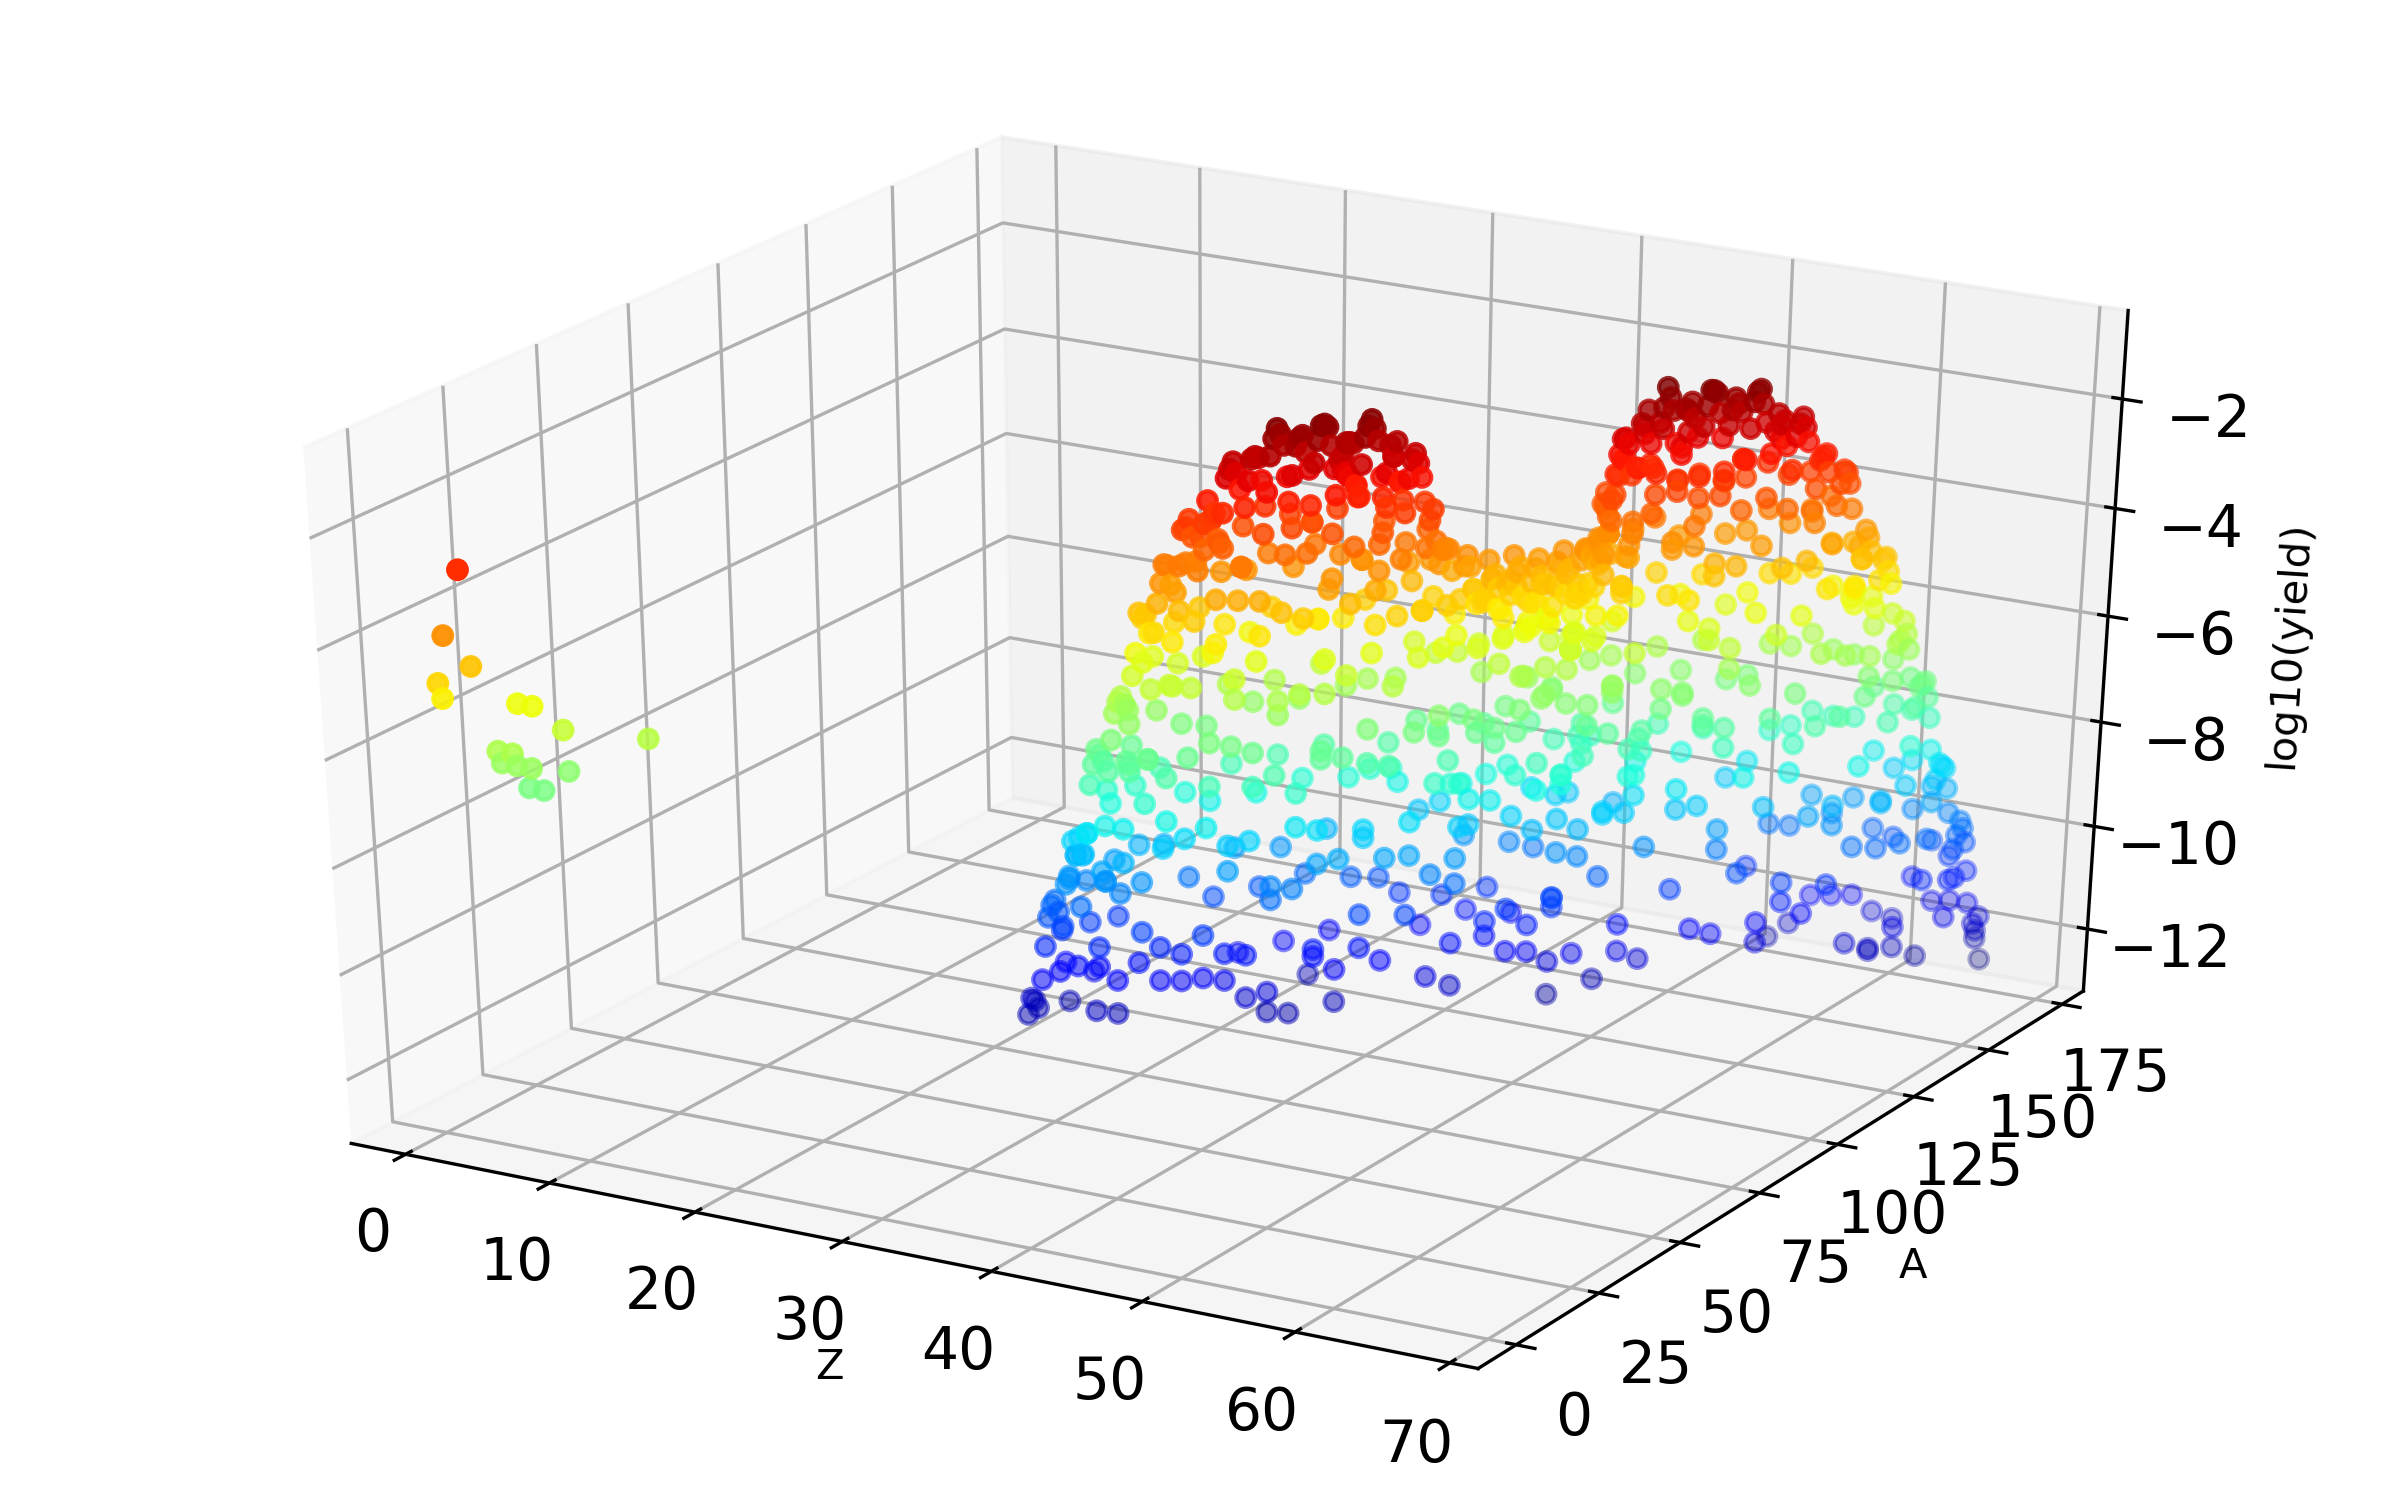
\includegraphics[scale=0.46] {figures/01-fissionyield3d-U235.png}
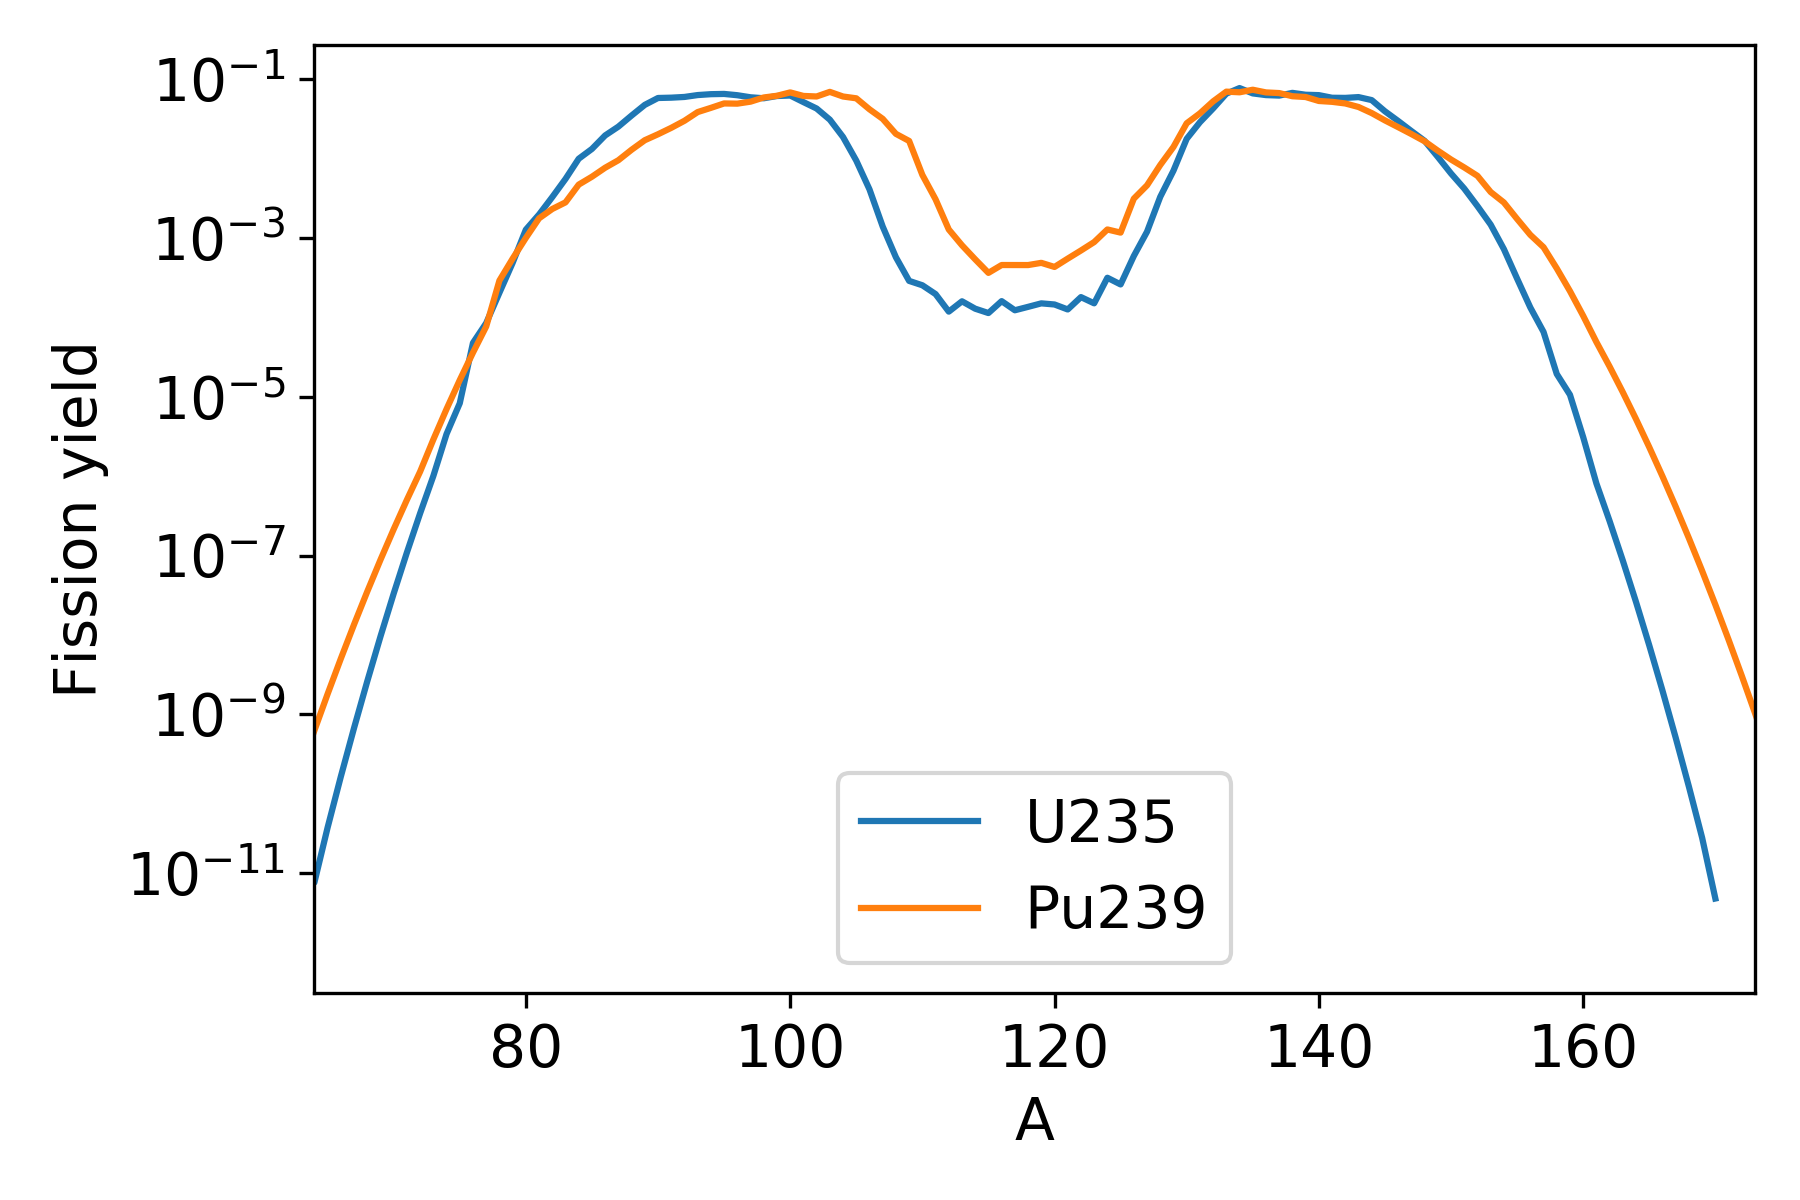
\includegraphics[scale=0.46] {figures/01-fissionyield2d.png}}\protect
\caption{\label{fig:fissyield} \footnotesize{Top: fission yield of U-235. Bottom: fission yield of U-235 and Pu-239 (both for thermal neutrons)}}
\end{figure}

Since the fission products are typically neutron rich, they undergo $beta$-decay, thus around 4-5\% of the energy is released in the form of radioactive decay with a time delay. A reactor core needs to be designed to be so that this decay heat can be removed from the system after the reactor is shutdown. The distribution of energy and where it is absorbed is given by the table below.

\begin{table}\caption{Distribution of energy in fission.}
\begin{tabular}{c | c | c | c}
Product & Energy (\%) & Range & Time delay \\
\hline
Fission product & 80 & short & prompt \\
Fast neutron & 3 & medium & prompt \\
Fission $\gamma$ & 4 & medium & prompt \\
$\beta$ decay & 4 & short & delayed \\
neutrinos & 5 & long & delayed \\
Non fission reactions & 4 &  & delayed 
\end{tabular}
\end{table}

Out of these events the short range events typically deposit the energy within the region the fission happened (ie. in the rod), therefore we need continuous cooling of the rods. Some of the energy is deposited farther from the source location (in the coolant, or in the shielding). As mentioned before the delayed component due to the radioactive decay of fission products requires the fuel to be cooled after the fission chain reaction is stopped in the reactor.

From the fission event several neutrons can be emitted, as we already discussed briefly, and soon will discuss in more detail, these neutrons make it possible to create a self-sustaining chain reactions, with the neutrons being chain carriers. Most of these neutrons are emitted almost instantaneously (within $10^{-14}$ s which is negligible compared to the time scales of neutron reactions), and are called prompt. But a small portion of neutrons (cca 0.6 \%) is emitted with a time delay.

The number of emitted neutrons (often noted with the greek letter $\nu$, and the average number as $\bar\nu$) varies between 0 and 6, with the most probable event being the emission of 2-3 neutrons as shown in Fig. \ref{fig:nu} for U-235. This distribution depends both on the nuclide and on the neutron energy. However, as one can see in the lower figure, the nubar is essentially constant for energies and nuclides relevant in light water reactors.

\begin{figure}[ht!]
\protect \centering{
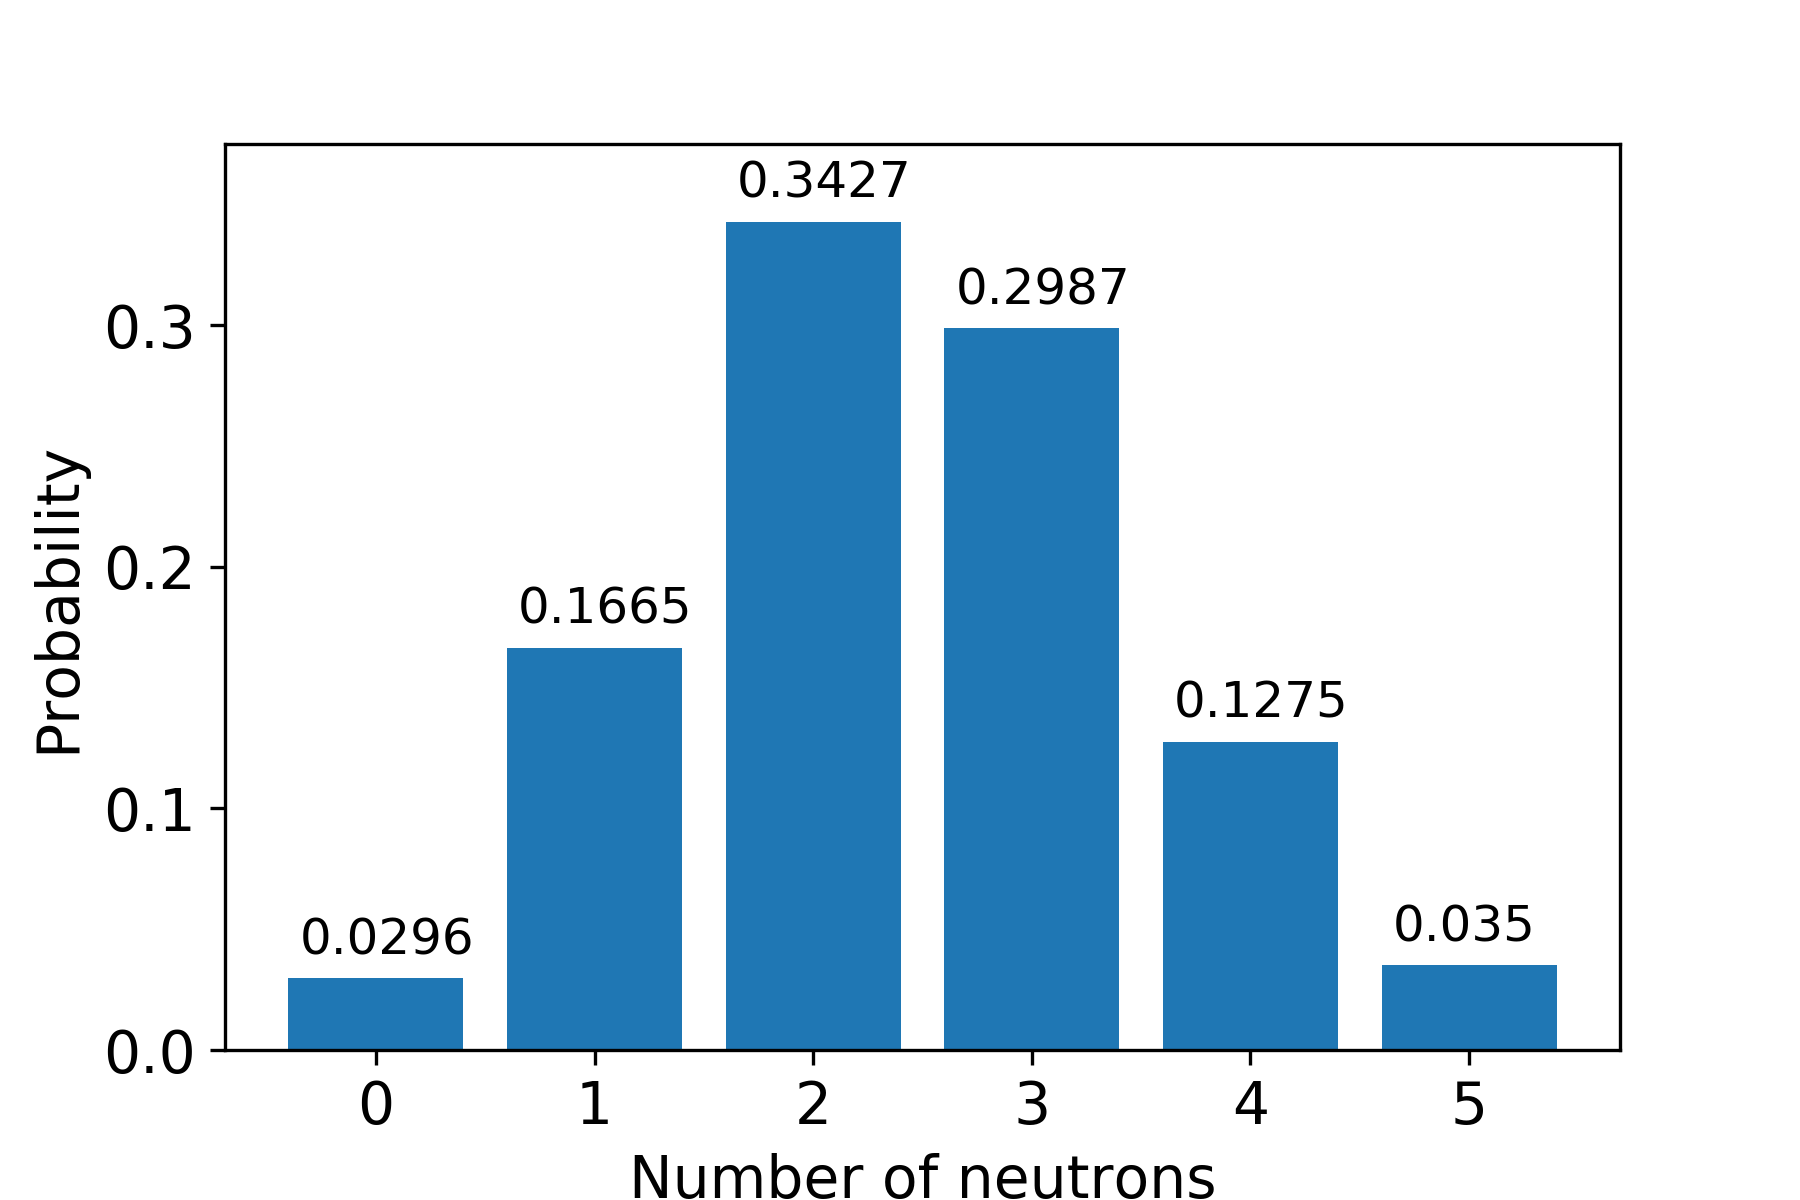
\includegraphics[scale=0.46] {figures/01-nu.png}
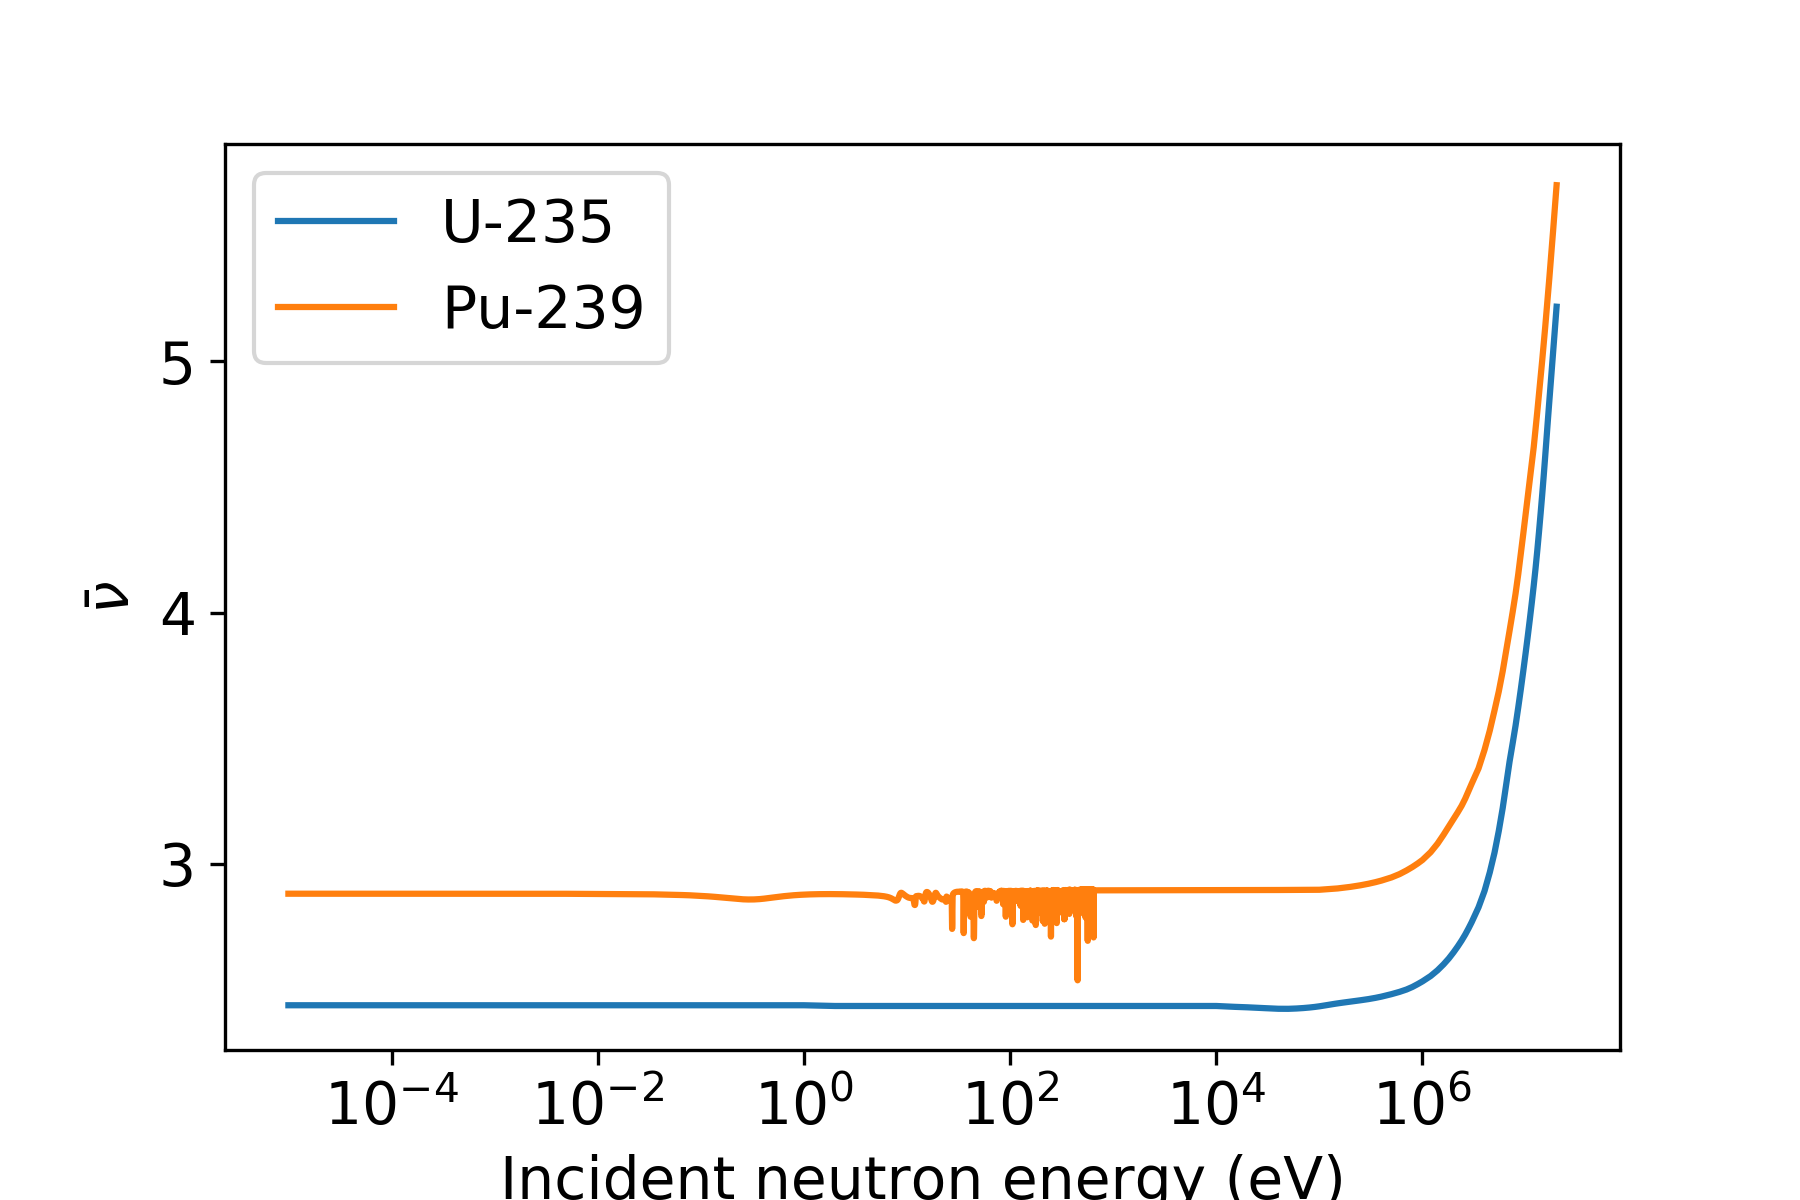
\includegraphics[scale=0.46] {figures/01-nubar.png}}\protect
\caption{\label{fig:nu} \footnotesize{Top: Number of emitted neutrons in the thermal fission of U-235. Bottom: Nubar of U-235 and Pu-239 vs the ingoing neutron energy.}}
\end{figure}

The energy distribution of the prompt fission neutron can be described by the semi-empirical Watt-spectrum 

\begin{equation}
\chi(E)=C_1\cdot \exp(-\frac{E}{C_2})\cdot \sinh(\sqrt{C_3\cdot E})
\end{equation}

\noindent where   $C_1 = 0.453$, $C_2 = 0.965$ and $C_3 = 2.29$ for U-235. $\chi(E)dE$ is the probability that the neutron after birth will have an energy between $[E,E+dE]$. The most probable neutron energy is cca. 0.85 MeV, and the average energy is 2 MeV. One can also observe from Fig. \ref{fig:watt} that birth neutron energies above 5 MeV are less probable, therefore in the future we can neglect some reactions, such as $(n,\textit{i}n)$ reactions which only happen with high energy neutrons). The birth energy spectrum is rather independent from the ingoing neutron energy, and is similar for most of the nuclides. For very detailed calculations one can take into account an event-by-event sampling of the birth energy (for example by taking into account that neutrons emitted from the same fission event have slightly correlated energies), but for us this simple model suffices. 

\begin{figure}[ht!]
\protect \centering{
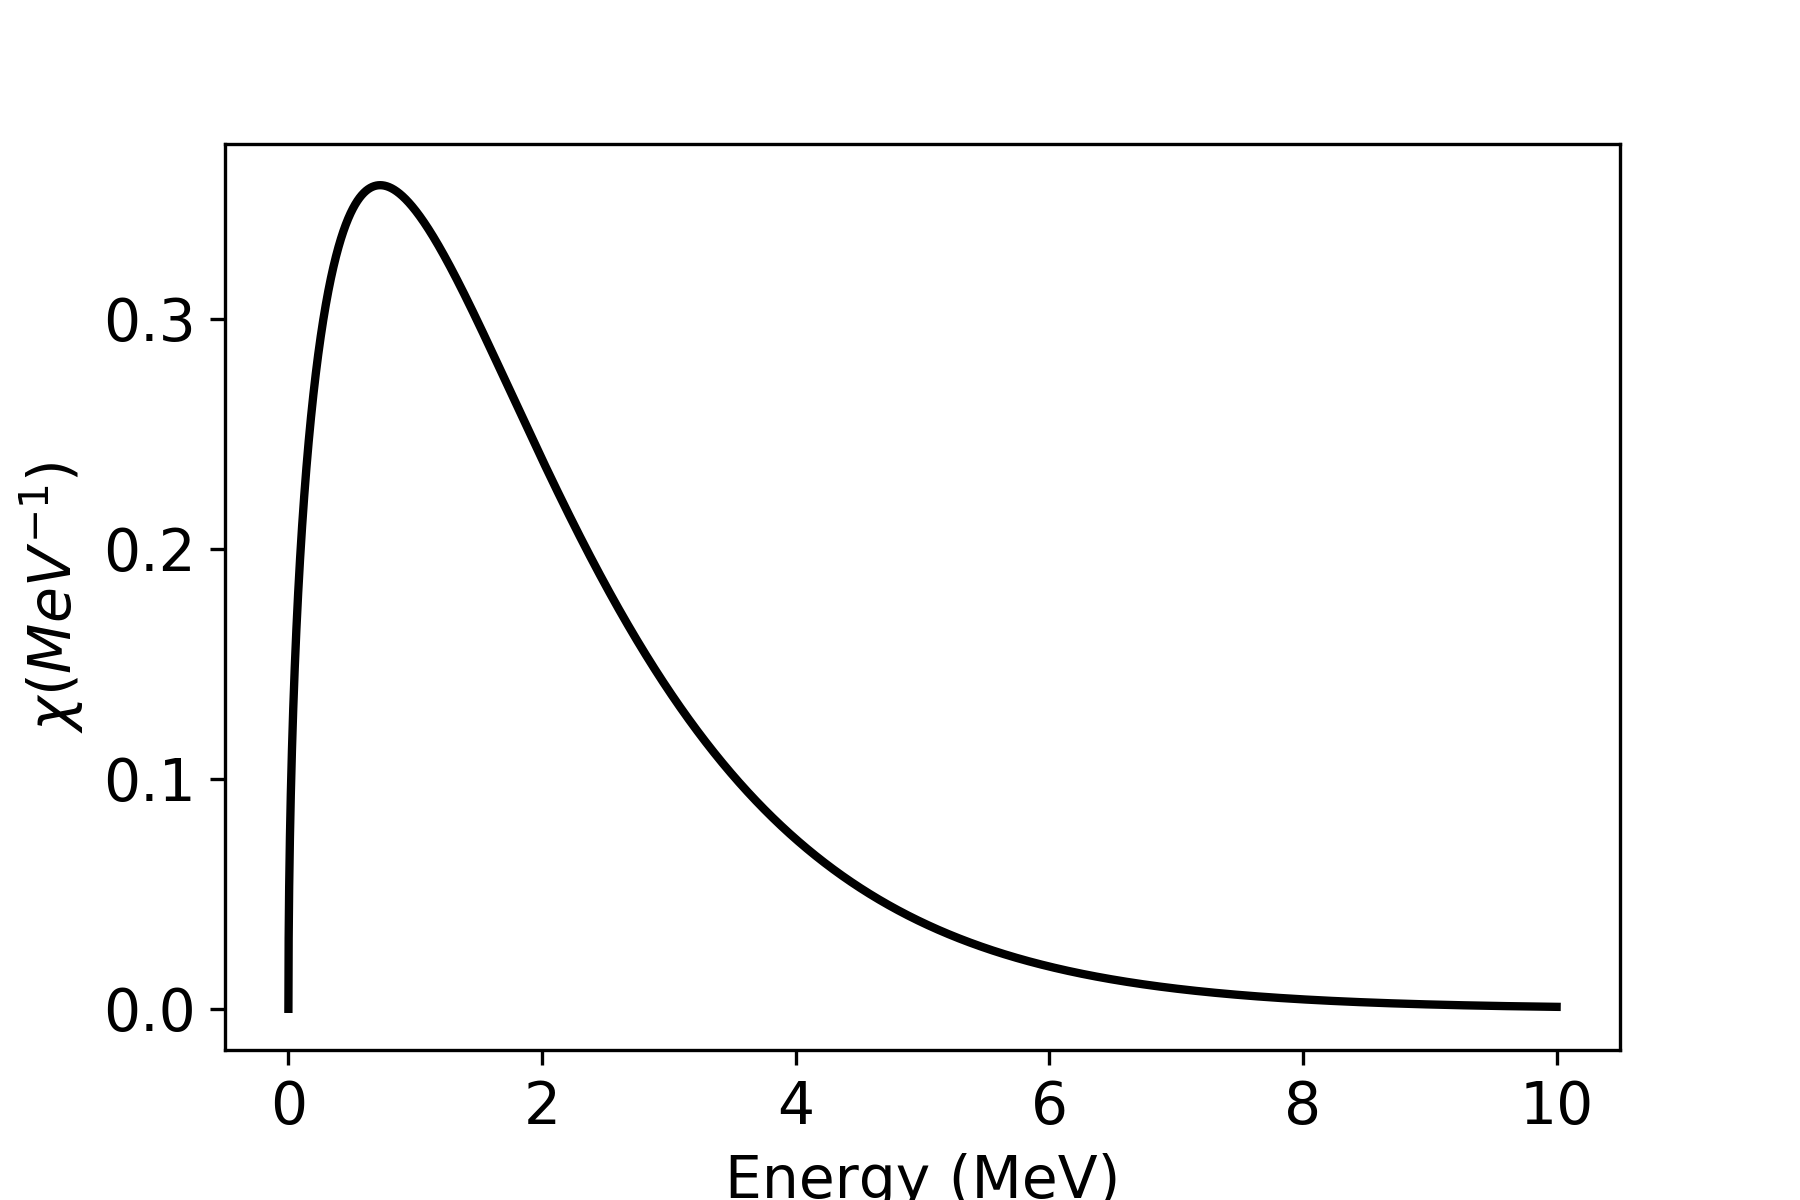
\includegraphics[scale=0.46] {figures/01-watt.png}}\protect
\caption{\label{fig:watt} \footnotesize{Top: The fission birth energy spectrum of neutrons for U235.}}
\end{figure}

\begin{figure}[ht!]
\protect \centering{
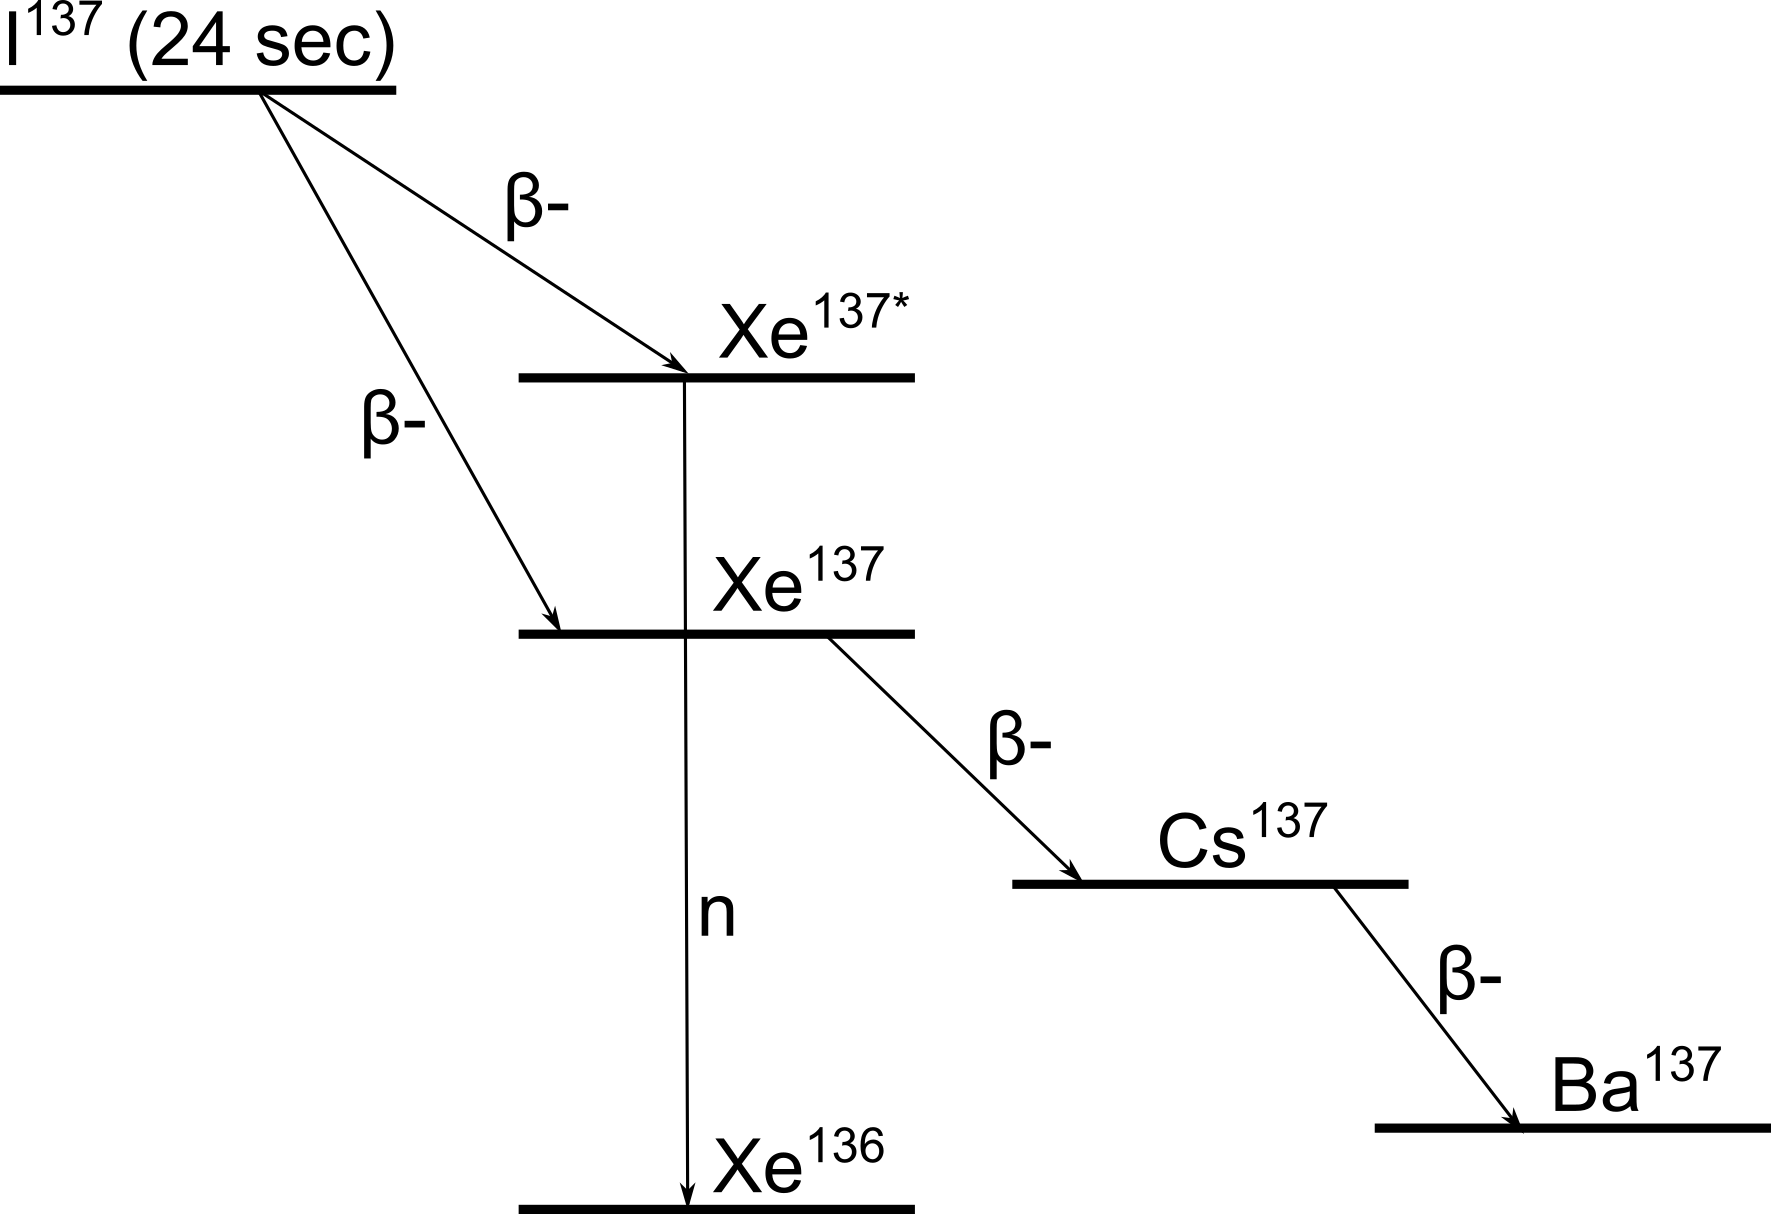
\includegraphics[scale=0.46] {figures/01-delayedexample.png}}\protect
\caption{\label{fig:delayedexample} \footnotesize{Example of delayed neutron emission: decay of I-137.}}
\end{figure}

As mentioned earlier some neutrons are emitted with a delay. An example of such delayed neutron emission is shown in Fig. \ref{fig:delayedexample}. I-137 is a fission product with a relatively high fission yield, after $\beta -$ decay it can disintegrate into the metastable state of Xe-137, which then is followed by the emission of a neutron. The time delay is characterized by the half-life of the original $\beta -$ decay (24 sec). We refer to the fission product which decays into the neutron emitting daughter as \textit{delayed neutron precursor}. There are tens of such precursors however in calculations they are usually grouped together into classes with similar half-lifes. Each of these groups can be characterized with

\begin{itemize}
\item $\lambda_i$ the decay constant of the \textit{i}th precursor group
\item $\beta_i$ fraction of all fission neutrons emitted per fission by the \textit{i}th precursor group
\end{itemize} 

The total fraction of delayed neutrons is

\[
\beta=\sum_i \beta_i
\]

and in some textbooks and data sources you can find the average number of delayed neutrons per fission to be given as

\[
\nu_d=\nu\beta
\]


The delayed neutron groups is available for various nuclides, and since the fission yields are different for nuclides, the groups and the total fraction of delated neutrons are also different. For plutonium isotopes the total fraction is generally lower. As we will see later when discussing transient events in nuclear reactors, the delayed neutrons although contributing with a low fraction have an enormous impact on the time response of the reactor. Delayed neutrons also have a slightly lower energies at birth than prompt neutrons. 

\begin{table}\caption{Delayed neutron fractions of U235}
\centering\begin{tabular}{c | c | c}
Group & $T_{1/2} (s)$ & $\beta_i\cdot 10^5$ \\
\hline
1 & 55.7 & 21 \\
2 & 22.7 & 142 \\
3 & 6.2 & 128 \\
4 & 2.3 & 257 \\
5 & 0.615 & 75 \\
6 & 0.23 & 27 
\end{tabular}
\end{table}

\subsubsection*{Fission fuels: effective number of neutrons}

We have already mentioned that certain nuclides are fissile, while others are fissionable. The only fissile isotope available in nature is U235, which is 0.711 w\% of natural uranium. As we saw ealier it is possible to use moderators with low absorption cross section (eg. heavy water) which allow for using natural uranium to build reactor cores, however more often uranium is enriched to contain a larger fraction of U235 than the natural abundance.

\begin{figure}[ht!]
\protect \centering{
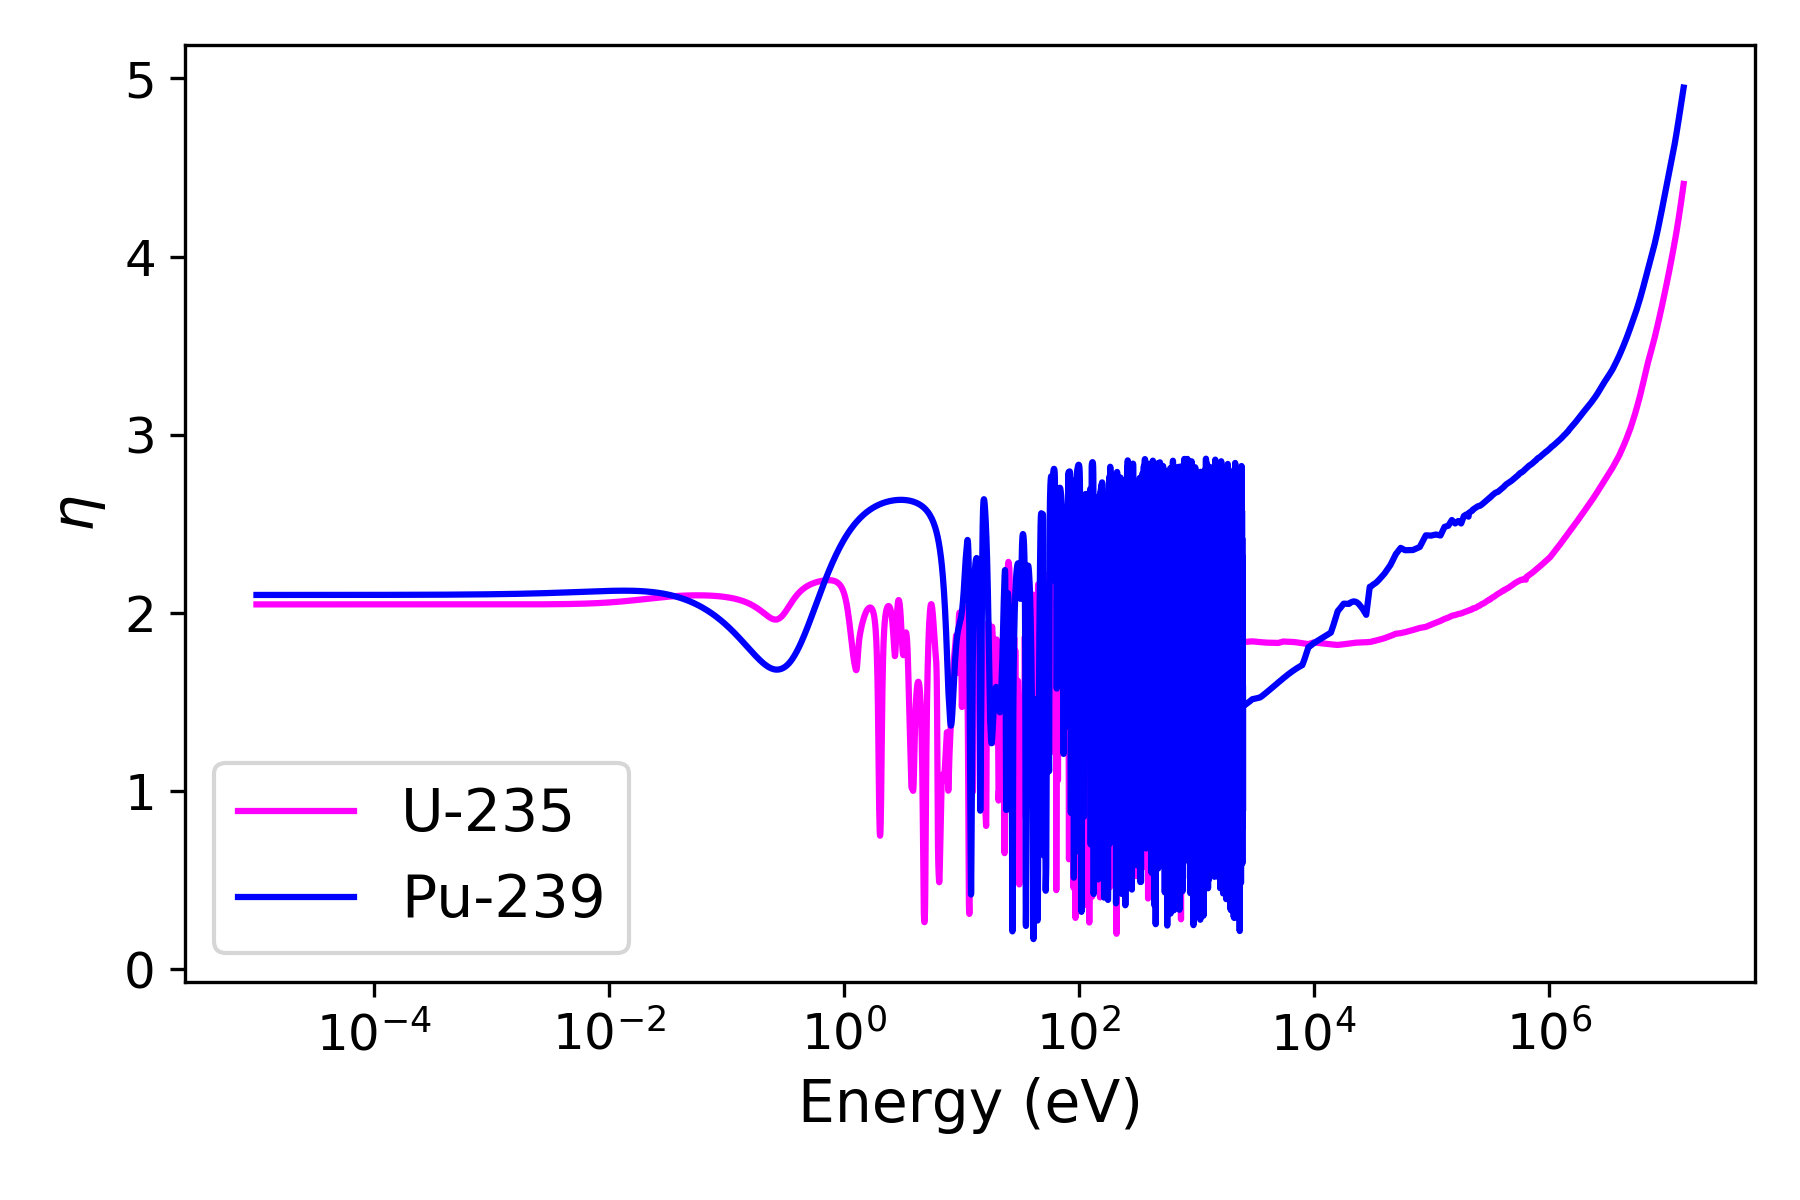
\includegraphics[scale=0.46] {figures/01-PuUeta.png}}\protect
\caption{\label{fig:eta} \footnotesize{Effective number of neutrons for U-235 and Pu-239.}}
\end{figure}

An other possibility is to breed fissile nuclides from fissionable (or due to this reason often called \textit{fertile} nuclides). One such reaction leading to the creation of fissile material in traditional LWR reactors is

\begin{equation}
{}^{238}U\xrightarrow[]{(n,\gamma)}{}^{239}U\xrightarrow[]{\beta^-(23.5m)}{}^{239}Np\xrightarrow[]{\beta^-(2.3d)} {}^{239}Pu
\end{equation}

If one wants to design a reactor which breeds more fissile material than what was initially placed into it (ie. a \textit{breeder} reactor) at least 1 neutron is needed to sustain the chain reaction, and one 1 is needed for breeding (while the rest can be lost due to other parasitic capture reactions. We can define the effective number of neutrons

\begin{equation}
\eta(E)=\nu(E)\frac{\sigma_f(E)}{\sigma_a(E)}
\end{equation}

\noindent which gives the average number of neutrons produced per neutron absorbed in the fuel. If the fuel consists of more nuclides (what is usually the case) we can similarly define

\[
\eta=\frac{\sum_j\nu_j\Sigma_f^j}{\sum_j\Sigma_a^j}
\]

The dependence of this quantity on the neutron energy is shown in Fig. \ref{fig:eta}. We can see that with increasing neutron energy the effective number of neutrons also increases. In order to achieve a self-sustaining chain reaction in a breeder reactor one needs

\begin{equation}
\bar\eta-1-\mathrm{parasitic}-\mathrm{leakage}\geq 1
\end{equation}

\noindent where the loss term is always positive, thus the minimum criterion for break-even breeding $\bar\eta\geq 2$. We can already see that in light water reactors this is very difficult to achieve.




%\end{document}